%
%  THESISBOEK
%
%  Dit bestand zorgt voor algemene (layout)definities, en groepeert de
%  afzonderlijke LaTeX-files tot een geheel.
%
%  @author Erwin Six, David De Reu, Brecht Vermeulen
%

\documentclass[12pt,a4paper,oneside,notitlepage]{book}
\usepackage[english,dutch]{babel}

\usepackage{subfiles}
\usepackage{fancyhdr}
\usepackage{graphicx,array, blindtext}
\usepackage{apalike}
\usepackage{pdfpages}
\usepackage{algorithmic}
%\usepackage{algorithmicx}
\usepackage{algorithm}
\usepackage{color}
\usepackage{booktabs}
\usepackage{url}
\usepackage{subcaption}
\usepackage{caption}
\usepackage{enumitem}
\usepackage{hyperref}
\usepackage[acronym,xindy,style=super, nonumberlist]{glossaries}
\usepackage{tikz}
\usepackage{amsthm}
\usepackage{amsfonts}
\usepackage{bbm}
\usepackage{amsmath}
\usepackage{varwidth}

\usetikzlibrary{automata}
\usetikzlibrary{decorations.pathreplacing}
\usetikzlibrary{shapes, arrows, shadows, positioning, backgrounds}
\usetikzlibrary{trees}

\definecolor{darkolivegreen}{rgb}{0.33, 0.42, 0.18}
\definecolor{officegreen}{rgb}{0.0, 0.5, 0.0}

\newcolumntype{L}[1]{>{\raggedright\let\newline\\\arraybackslash\hspace{0pt}}m{#1}}
\newcolumntype{C}[1]{>{\centering\let\newline\\\arraybackslash\hspace{0pt}}m{#1}}
\newcolumntype{R}[1]{>{\raggedleft\let\newline\\\arraybackslash\hspace{0pt}}m{#1}}

\renewcommand{\algorithmicrequire}{\textbf{Input:}}
\renewcommand{\algorithmicensure}{\textbf{Output:}}
\renewcommand{\algorithmiccomment}[1]{\textcolor{officegreen}{// #1}}

\newcommand\tab[1][1cm]{\hspace*{#1}}
% \usepackage[colorlinks]{hyperref}

% marges aanpassen
% (opmerking: moet *voor* inclusie van fancyhdr package komen)
\setlength{\hoffset}{-1in}
\setlength{\voffset}{-1in}
\setlength{\topmargin}{2cm}
\setlength{\headheight}{0.5cm}
\setlength{\headsep}{1cm}
\setlength{\oddsidemargin}{3.5cm}
\setlength{\evensidemargin}{3.5cm}
\setlength{\textwidth}{16cm}
\setlength{\textheight}{23.3cm}
\setlength{\footskip}{1.5cm}
\setlength{\parindent}{0pt} % No indentation at the beginning of a paragraph
\setlist{noitemsep}

\pagestyle{fancy}

\tikzstyle{state}=[shape=circle,draw=black!50,scale=2.0]
\tikzstyle{staterect}=[shape=rectangle,draw=black!50]
\tikzstyle{state_small}=[shape=circle,draw=black!50,scale=1.5]
\tikzstyle{state2}=[minimum width=8pt,shape=circle,draw=blue!50,fill=blue!20]
\tikzstyle{observation}=[shape=rectangle,draw=orange!50,fill=orange!20]
\tikzstyle{lightedge}=[<-,dotted]
\tikzstyle{mainstate}=[state,thick]
\tikzstyle{mainedge}=[<-,thick]

\newtheorem{definition}{Definition}
\newtheorem{theorem}{Theorem}
\newtheorem{example}{Example}

\newcommand{\npar}{\vspace{0.5cm} \par \noindent}
\renewcommand{\chaptermark}[1]{\markright{\MakeUppercase{#1}}}
\renewcommand{\sectionmark}[1]{\markright{\thesection~#1}}

\newcommand{\headerfmt}[1]{\textsl{\textsf{#1}}}
\newcommand{\headerfmtpage}[1]{\textsf{#1}}
\renewcommand{\glsnamefont}[1]{\textbf{#1}}

\fancyhf{}
\fancyhead[LE,RO]{\headerfmtpage{\thepage}}
\fancyhead[LO]{\headerfmt{\rightmark}}
\fancyhead[RE]{\headerfmt{\leftmark}}
\renewcommand{\headrulewidth}{0.5pt}
\renewcommand{\footrulewidth}{0pt}

\fancypagestyle{plain}{ % eerste bladzijde van een hoofdstuk
  \fancyhf{}
  \fancyhead[LE,RO]{\headerfmtpage{\thepage}}
  \fancyhead[LO]{\headerfmt{\rightmark}}
  \fancyhead[RE]{\headerfmt{\leftmark}}
  \renewcommand{\headrulewidth}{0.5pt}
  \renewcommand{\footrulewidth}{0pt}
}

% anderhalve interlinie (opm: titelblad gaat uit van 1.5)
\renewcommand{\baselinestretch}{1.19}



% indien LaTeX niet goed splitst, neem je woord hierin op, of evt om splitsen 
% te voorkomen
\hyphenation{ditmagnooitgesplitstworden dit-woord-splitst-hier}

\makeglossaries
\makeglossary
\loadglsentries{acronyms}

\begin{document}

\selectlanguage{english}

% titelblad (voor kaft)
%% %  Titelblad

% % Opmerking: gaat uit van een \baselinestretch waarde van 1.5 (die moet
% % ingesteld worden voor het begin van de document environment)

% \begin{titlepage}

% \setlength{\hoffset}{-1in}
% \setlength{\voffset}{-1in}
% \setlength{\topmargin}{1.5cm}
% \setlength{\headheight}{0.5cm}
% \setlength{\headsep}{1cm}
% \setlength{\oddsidemargin}{3cm}
% \setlength{\evensidemargin}{3cm}
% \setlength{\footskip}{1.5cm}
% \enlargethispage{1cm}
% % \textwidth en \textheight hier aanpassen blijkt niet te werken

% \fontsize{12pt}{14pt}
% \selectfont

% \begin{center}

% 
\includegraphics[height=4cm]{fig/logo_ugent}

% \vspace{0.5cm}

% \vspace{2.5cm}

% \fontseries{bx}
% \fontsize{17.28pt}{21pt}
% \selectfont

% Teaching Computers to Play Chess Through \\
% Deep Reinforcement Learning

% \fontseries{m}
% \fontsize{12pt}{14pt}
% \selectfont

% \vspace{.6cm}

% by 

% \vspace{.4cm}

% Dorian Van den Heede

% \vspace{2.5cm}

% Thesis submitted to the faculty of \\
% Engineering \& Architecture, University of Ghent,\\
% in partial fulfillment of the requirements for the degree of \\
% Master of Science in Computer Science Engineering

% \vspace{1.5cm}

% Supervisor: Prof.~Dr.~Ir.~F.~wyffels\\
% Counsellor: Ir.~J.~Burms\\

% \vspace{2cm}

% %Scriptie ingediend tot het behalen van de academische graad van\\
% %burgerlijk ingenieur in de computerwetenschappen

% \vspace{1cm}

% 2016-2017

% \end{center}
% \end{titlepage}


\setlength{\voffset}{0in}
\setlength{\hoffset}{0in}
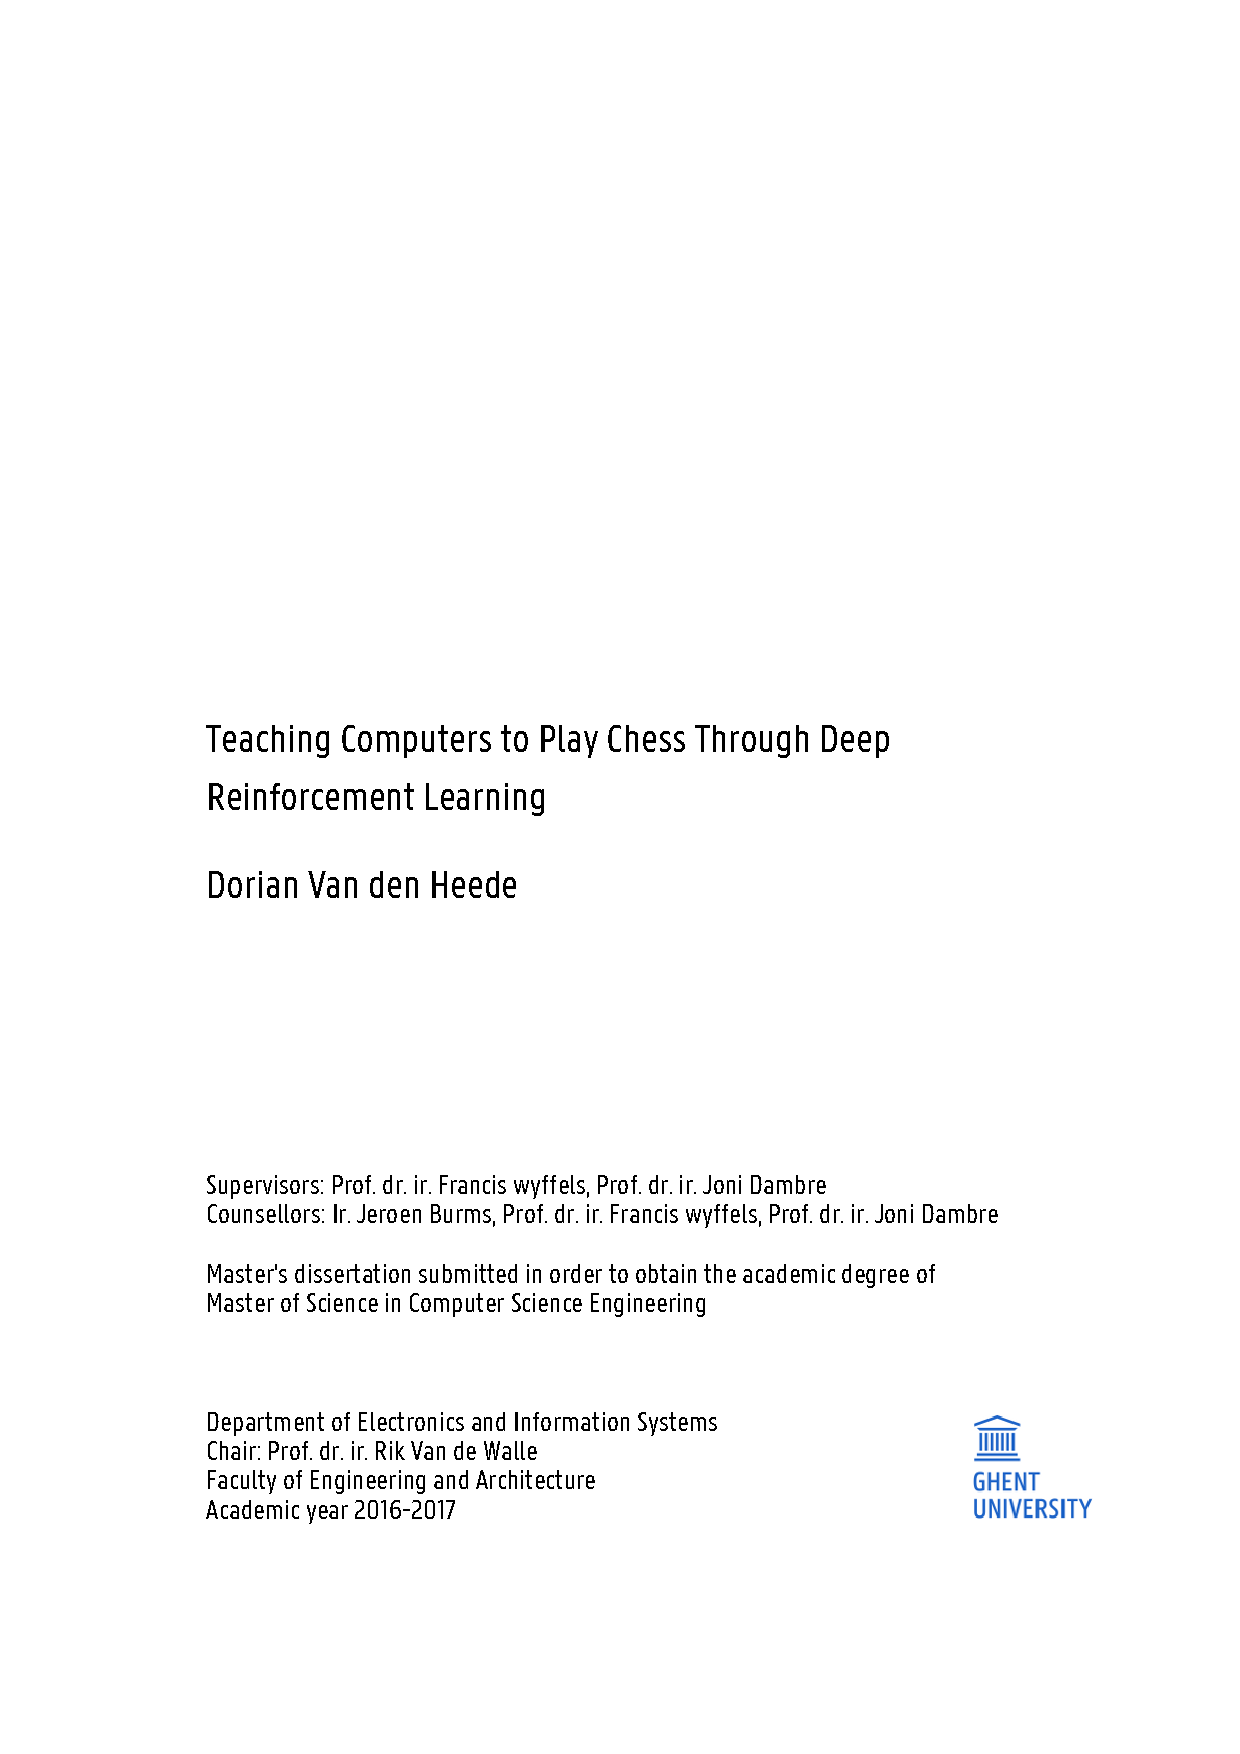
\includepdf[pages={1}]{title_thesis.pdf}
\color{white}
To be, or not to be: that is the question: 
Whether 'tis nobler in the mind to suffer 
The slings and arrows of outrageous fortune, 
Or to take arms against a sea of troubles,		
And by opposing end them? To die: to sleep; 
No more; and by a sleep to say we end 
The heart-ache and the thousand natural shocks
That flesh is heir to, 'tis a consummation 
Devoutly to be wish'd. To die, to sleep;
To sleep: perchance to dream: ay, there's the rub;
For in that sleep of death what dreams may come 
When we have shuffled off this mortal coil, 
Must give us pause: there's the respect 
That makes calamity of so long life;	
For who would bear the whips and scorns of time,
The oppressor's wrong, the proud man's contumely, 
The pangs of disprized love, the law's delay, 
The insolence of office and the spurns 
That patient merit of the unworthy takes, 
When he himself might his quietus make 
With a bare bodkin? who would fardels bear, 
To grunt and sweat under a weary life, 
But that the dread of something after death,
The undiscover'd country from whose bourn 
No traveller returns, puzzles the will 
And makes us rather bear those ills we have 
Than fly to others that we know not of?	
Thus conscience does make cowards of us all; 
And thus the native hue of resolution 
Is sicklied o'er with the pale cast of thought,
And enterprises of great pith and moment 
With this regard their currents turn awry, 
And lose the name of action.
\color{black}
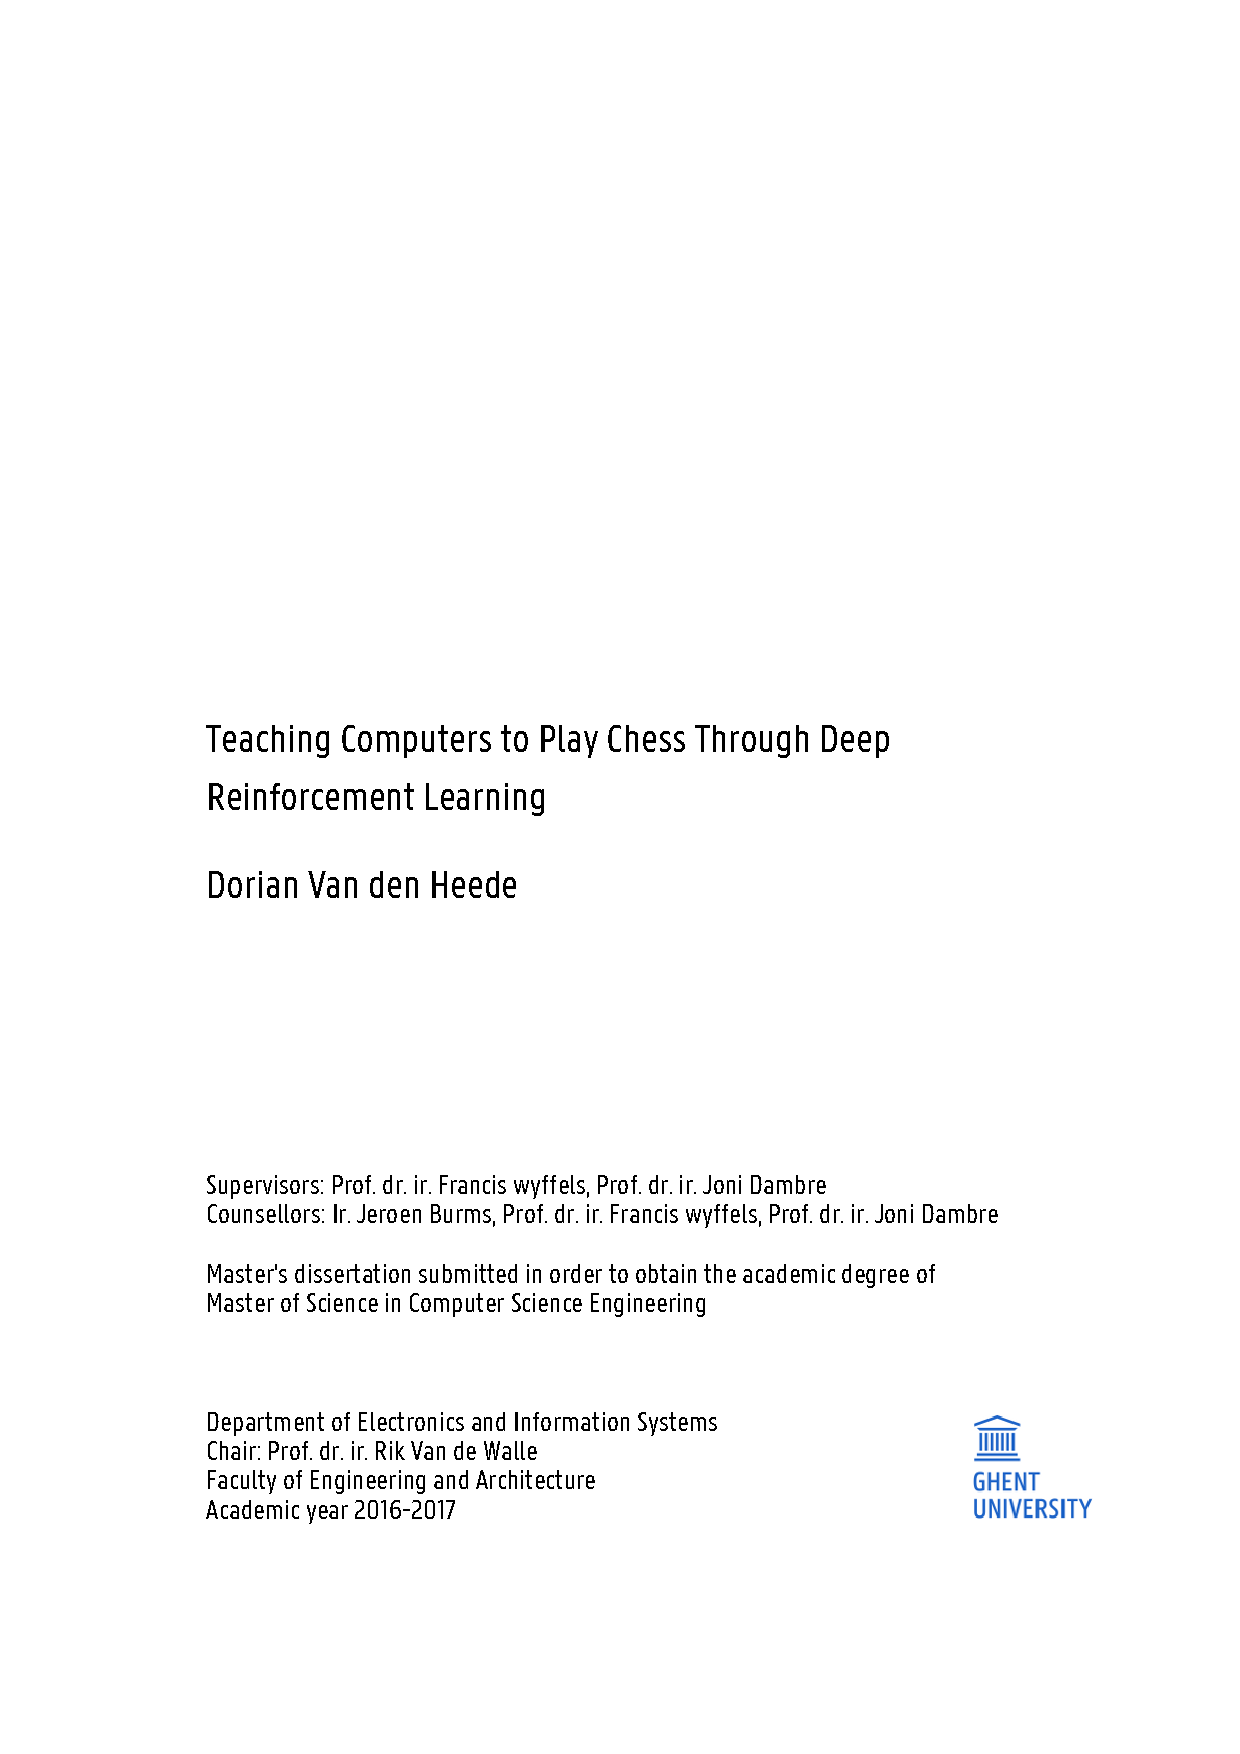
\includepdf[pages={1}]{title_thesis.pdf}
\setlength{\voffset}{-1in}
\setlength{\hoffset}{-1in}

% lege pagina (!!)

% titelblad (!!)

% geen paginanummering tot we aan de inhoudsopgave komen
\pagestyle{empty}

% voorwoord met dankwoord en toelating tot bruikleen (ondertekend)
%%  Voorwoord (dankwoord) en toelating tot bruikleen

\begin{slshape}
\subsection*{Foreword}
\renewcommand{\baselinestretch}{1.2}
\small\normalsize

\npar 
After a long and sporadically lonesome road, an incredible journey has come to an end in the form of this master dissertation. Exploiting experience from exploration is what makes one fail less and less. \\

I had the amazing opportunity to pursue my thesis in a subject I am extremely passionate about, for which I want to thank my supervisor Prof. Francis wyffels.\\

Last year and especially the last three months, I needed a lot of advice and help. Luckily, Jeroen Burms has always been a great counselor and helped me whenever I had a question or idea. Thank you.\\

I want to express my gratitude to 'grand papa et grand maman'. During the fortnight of my isolation, they spoiled me more than my facebook wall spoiled the Game of Thrones story.\\

Furthermore I want to show appreciation to my fellow students with whom I spent countless hours of hard labor. I am thanking Jonas for lifting me up, Loic for always remaining casual, Timon for always being equally happy and Vincent for infecting invincibility.\\

Closer to me, there are my parents whom I love very much. I am sincerely sorry if I do not show this enough.\\

\noindent Dorian Van den Heede, august 2017
\end{slshape}

\newpage
\section*{Permission of use on loan}

\vspace{1.5cm}

\noindent
``The author(s) gives (give) permission to make this master dissertation available for consultation
and to copy parts of this master dissertation for personal use.
 In the case of any other use, the copyright terms have to be respected, in particular with regard to
the obligation to state expressly the source when quoting results from this master dissertation.''

\addvspace{4cm}

\noindent Dorian Van den Heede, august 2017


% overzicht
%%  Overzichtsbladzijde met samenvatting

\newpage

{
\setlength{\baselineskip}{14pt}
\setlength{\parindent}{0pt}
\setlength{\parskip}{8pt}

\begin{center}

\noindent \textbf{\huge
Ontwerp van een performante\\[8pt]
gedistribueerde CORBA--monitor
}

door 

David DE REU

Scriptie ingediend tot het behalen van de academische graad van\\
burgerlijk ingenieur in de computerwetenschappen

Academiejaar 2001--2002

Promotor: Prof.~Dr.~Ir.~P.~DEMEESTER\\
Scriptiebegeleider: Ir.~B.~VERMEULEN

Faculteit Toegepaste Wetenschappen\\
Universiteit Gent

Vakgroep Informatietechnologie\\
Voorzitter: Prof.~Dr.~Ir.~P.~LAGASSE

\end{center}

\section*{Samenvatting}

% TODO: samenvatting

Hier komt de samenvatting.


\section*{Trefwoorden}

% TODO: trefwoorden

Hier komen trefwoorden.

}

\newpage % strikt noodzakelijk om een header op deze blz. te vermijden


\pagestyle{fancy}
\frontmatter
\color{white}
To be, or not to be: that is the question: 
Whether 'tis nobler in the mind to suffer 
The slings and arrows of outrageous fortune, 
Or to take arms against a sea of troubles,		
And by opposing end them? To die: to sleep; 
No more; and by a sleep to say we end 
The heart-ache and the thousand natural shocks
That flesh is heir to, 'tis a consummation 
Devoutly to be wish'd. To die, to sleep;
To sleep: perchance to dream: ay, there's the rub;
For in that sleep of death what dreams may come 
When we have shuffled off this mortal coil, 
Must give us pause: there's the respect 
That makes calamity of so long life;	
For who would bear the whips and scorns of time,
The oppressor's wrong, the proud man's contumely, 
The pangs of disprized love, the law's delay, 
The insolence of office and the spurns 
That patient merit of the unworthy takes, 
When he himself might his quietus make 
With a bare bodkin? who would fardels bear, 
To grunt and sweat under a weary life, 
But that the dread of something after death,
The undiscover'd country from whose bourn 
No traveller returns, puzzles the will 
And makes us rather bear those ills we have 
Than fly to others that we know not of?	
Thus conscience does make cowards of us all; 
And thus the native hue of resolution 
Is sicklied o'er with the pale cast of thought,
And enterprises of great pith and moment 
With this regard their currents turn awry, 
And lose the name of action.
\color{black}
\addcontentsline{toc}{chapter}{Preface}
%  Voorwoord (dankwoord) en toelating tot bruikleen

\begin{slshape}
\subsection*{Foreword}
\renewcommand{\baselinestretch}{1.2}
\small\normalsize

\npar 
After a long and sporadically lonesome road, an incredible journey has come to an end in the form of this master dissertation. Exploiting experience from exploration is what makes one fail less and less. \\

I had the amazing opportunity to pursue my thesis in a subject I am extremely passionate about, for which I want to thank my supervisor Prof. Francis wyffels.\\

Last year and especially the last three months, I needed a lot of advice and help. Luckily, Jeroen Burms has always been a great counselor and helped me whenever I had a question or idea. Thank you.\\

I want to express my gratitude to 'grand papa et grand maman'. During the fortnight of my isolation, they spoiled me more than my facebook wall spoiled the Game of Thrones story.\\

Furthermore I want to show appreciation to my fellow students with whom I spent countless hours of hard labor. I am thanking Jonas for lifting me up, Loic for always remaining casual, Timon for always being equally happy and Vincent for infecting invincibility.\\

Closer to me, there are my parents whom I love very much. I am sincerely sorry if I do not show this enough.\\

\noindent Dorian Van den Heede, august 2017
\end{slshape}

\newpage
\section*{Permission of use on loan}

\vspace{1.5cm}

\noindent
``The author(s) gives (give) permission to make this master dissertation available for consultation
and to copy parts of this master dissertation for personal use.
 In the case of any other use, the copyright terms have to be respected, in particular with regard to
the obligation to state expressly the source when quoting results from this master dissertation.''

\addvspace{4cm}

\noindent Dorian Van den Heede, august 2017


\addcontentsline{toc}{chapter}{Abstract}
%%%%%%%%%%%%%%%%%%%%%%%%%%  phdsymp_sample2e.tex %%%%%%%%%%%%%%%%%%%%%%%%%%%%%%
%% changes for phdsymp.cls marked with !PN
%% except all occ. of phdsymp.sty changed phdsymp.cls
%%%%%%%%%%                                                       %%%%%%%%%%%%%
%%%%%%%%%%    More information: see the header of phdsymp.cls   %%%%%%%%%%%%%
%%%%%%%%%%                                                       %%%%%%%%%%%%%
%%%%%%%%%%%%%%%%%%%%%%%%%%%%%%%%%%%%%%%%%%%%%%%%%%%%%%%%%%%%%%%%%%%%%%%%%%%%%%%


%\documentclass[10pt]{phdsymp} %!PN
\documentclass[twocolumn]{phdsymp} %!PN
%\documentclass[12pt,draft]{phdsymp} %!PN
%\documentstyle[twocolumn]{phdsymp}
%\documentstyle[12pt,twoside,draft]{phdsymp}
%\documentstyle[9pt,twocolumn,technote,twoside]{phdsymp}

\usepackage[english]{babel}       % Voor nederlandstalige hyphenatie (woordsplitsing)
\usepackage{tikz}
\usepackage{url}
\usepackage{graphicx}
\usepackage[tablename=Tab.]{caption}
\usepackage{subcaption}
\captionsetup{compatibility=false}
\usepackage[acronym,xindy,style=super, nonumberlist]{glossaries}
\graphicspath{{figuren/}}               % De plaats waar latex zijn figuren gaat halen.
\usepackage{booktabs}
\usepackage{times}
\usepackage{amsfonts}
\usepackage{bbm}
\usepackage{amsmath,scalefnt}

\usetikzlibrary{automata}
\usetikzlibrary{decorations.pathreplacing}
\usetikzlibrary{shapes, arrows, shadows, positioning, backgrounds}
\usetikzlibrary{trees}
\tikzstyle{state}=[shape=circle,draw=black!50,scale=2.0]
\tikzstyle{staterect}=[shape=rectangle,draw=black!50]
\tikzstyle{state_small}=[shape=circle,draw=black!50,scale=1.5]
\tikzstyle{state2}=[minimum width=8pt,shape=circle,draw=blue!50,fill=blue!20]
\tikzstyle{observation}=[shape=rectangle,draw=orange!50,fill=orange!20]
\tikzstyle{lightedge}=[<-,dotted]
\tikzstyle{mainstate}=[state,thick]
\tikzstyle{mainedge}=[<-,thick]

\hyphenation{si-mu-la-ted re-a-lis-tic packets really in-clu-ding}

\def\BibTeX{{\rm B\kern-.05em{\sc i\kern-.025em b}\kern-.08em
    T\kern-.1667em\lower.7ex\hbox{E}\kern-.125emX}}

\newtheorem{theorem}{Theorem}

\makeglossaries
\newacronym{drl}{DRL}{deep reinforcement learning}
\newacronym{sl}{SL}{supervised learning}
\newacronym{td}{TD}{temporal difference}
\newacronym{ai}{AI}{artificial intelligence}
\newacronym{sota}{SOTA}{state of the art}
\newacronym{rl}{RL}{reinforcement learning}
\newacronym{cnn}{CNN}{convolutional neural network}
\newacronym{nn}{NN}{neural network}
\newacronym{fnn}{FNN}{feedforward neural network}
\newacronym{mdp}{MDP}{Markov decision process}
\newacronym{mse}{MSE}{mean squared error}
\newacronym{sgd}{SGD}{stochastic gradient descent}
\newacronym{pv}{PV}{principal variation}
\newacronym{fcn}{FCN}{fully connected network}
\newacronym{dtm}{DTM}{depth to mate}
\newacronym{wdl}{WDL}{win draw loss}
\newacronym{krk}{KRK}{king rook king}
\newacronym{kqk}{KQK}{king queen king}
\newacronym{wcr}{WCR}{win conversion rate}
\newacronym{we}{WE}{win efficiency}
\newacronym{lhs}{LHS}{loss holding score}
\newacronym{relu}{ReLU}{rectifier linear unit}
\captionsetup{tablename=Tab.}
\begin{document}

\title{Teaching Computers to Play Chess with Deep Reinforcement Learning} %!PN

\author{Dorian Van den Heede}

\supervisor{Francis wyffels, Jeroen Burms, Joni Dambre}

\maketitle

\begin{abstract}
Chess computers have reached a superhuman level at playing chess by combining tree search with the incorporation of heuristics obtained with expert knowledge into the value function when evaluating board positions. Although these approaches add a big amount of tactical knowledge, they do not tackle the problem of effectively solving chess, a deterministic game. We try to set the first stone by solving relatively simple chess endgames from a human point of view with \gls{drl}. The proposed \gls{drl} algorithm consists of 2 main components: (i) self play (ii) translating the collected data in phase (i) to a \gls{sl} framework with deep learning. In light of this, we present a novel \gls{td} learning algorithm, TD-Stem($\lambda$), and compare it with the state of the art, TD-Leaf($\lambda$).
\end{abstract}

\begin{keywords}
Chess, deep reinforcement learning, TD-learning
\end{keywords}

\section{Introduction}
\PARstart{I}{n} the early 50s, scientists like Shannon and Turing were already musing about how a machine would be able to play chess autonomously \cite{shannon,turing}. The enormous complexity ($\sim 10^{120}$ different states) combined with its popularity and rich history made it the holy grail of \gls{ai} research in the second half of the $20^{\textnormal{th}}$ century. Research attained its peak in 1997 when \textit{Deep Blue} succeeded at winning a duel with the human world champion at that time, \textit{Gary Kasparov} \cite{deepblue}. Conventional chess computers now attain a superhuman level.\\
Current \gls{sota} engines use a combination of deep search trees with expert knowledge heuristics to evaluate positions at leaf nodes (\textit{Komodo},\textit{Stockfish} and \textit{Houdini} at time of writing) \cite{sota}. Furthermore, the search is heavily optimized as an attempt to reduce the influence of the exponentially increasing complexity when looking more moves ahead. The height of the search tree is the most crucial factor for the performance of an engine. These observations lead to the following shortcomings: (i) the strategic strength is entirely based on the heuristical evaluation at leaf nodes, which is humanly biased and suboptimal as a consequence (ii) conventional play by engines is very tactical as the reached depth is the most important variable for performance, resulting in a lack of intuitive game play (iii) as current engines mostly rely on human insight, they do not take steps at objectively solving the game, but more at how to beat humans with their advantage in calculation power.\\
These downsides could eventually be solved by looking at the game in a primitive and unbiased viewpoint and using a combination of self play with supervised machine learning in a \gls{rl} framework. As a first step we have implemented a deep learning architecture where we use a novel TD-learning variant in combination with neural networks being fed by positions represented as bitboards.\\
This paper is organized as follows. In section \ref{sec:relwork} a brief overview of previous research in this domain is given. Section \ref{sec:drl} introduces the used \gls{drl} framework after which we focus on how different modifications of the well known TD($\lambda$) algorithm may unite strategic and tactical information into the value function in section \ref{sec:td}. The value function itself is discussed in \ref{sec:nn}. We compare our novel algorithm with the \gls{sota} TD-learning algorithm for chess in section \ref{sec:res} and form an appropriate conclusion in section \ref{sec:con}.

\section{Related Work}
\label{sec:relwork}
Already in 1959, a TD-learning algorithm was used to create a simplistic checkers program \cite{samuel}. The first real success story of using TD-learning (arguably for \gls{rl} in general) and \Gls{nn} for value function approximation in boardgames was \textit{Tesouro}'s backgammon program \textit{TD-Gammon} with a simple fully connected \gls{fnn} architecture learned by incremental TD($\lambda$) updates \cite{tesauro}. One interesting consequence of \textit{TD-Gammon} is its major influence on strategic game play of humans in backgammon today. As chess is a game where tactics seem to have the upper hand over strategic thinking, game tree search is used to calculate the temporal difference updates in TD-Leaf($\lambda$) proposed by \textit{Baxter} et al. The chess software \textit{KnightCap} that came out of it used linear expert knowledge board features for function approximation and had learned to play chess up until master level by playing on a chess server. The same method was used in combination with a two layer \gls{nn} initialized with biased piece value knowledge in \textit{Giraffe} to reach grandmaster level, effectively proving the potential strength of TD-learning methods with search at a limited depth \cite{giraffe}.  Veness et al.went even further and stored as much information from game tree search during self play as possible in \textit{Meep} \cite{meep}.\\
The potential of using millions of database games between experts to learn to play chess has been exploited in \textit{DeepChess} \cite{deepchess}.\\

In \gls{rl} research concerning other games, \glspl{cnn} have already been proven its worth. A lot of research has been undertaken to Atari video games, which makes sense as \glspl{cnn} were originally designed for computer vision tasks \cite{atari}. The current \gls{sota} is a dual network learning the advantage function with double deep Q-learning \cite{dddqn}. The first successful application of \Gls{cnn} into boardgames is \textit{AlphaGo}, which is the first \textit{Go} program to beat a player with the highest possible rating \cite{alphago}.   

\section{Deep Reinforcement Learning Framework for Chess}
\label{sec:drl}
Our system consists out of two main components, namely self play and the incorporation of newly seen data into the system. These two phases are performed iteratively. In section \ref{sec:rl} chess is formulated as an \gls{rl} framework. The system updates are explained with the help of an \gls{sl} framework in section \ref{sec:sl}.

\subsection{Reinforcement Learning}
\label{sec:rl}
In \gls{rl}, agents are released in an environment where they have to find out by exploration which actions generate the best cumulative rewards. In this case, the board is the environment and white and black are the agents. When one player succeeds at mating the opponent, a positive reward is provided.\\
To this cause, we have to model chess as a deterministic \gls{mdp} $\mathcal{M}=(\mathcal{S},\mathcal{A}$ $,r,\gamma)$ with \cite{rl}
\begin{itemize}
\item $\mathcal{S}$: state space containing all possible board positions
\item $\mathcal{A}$: action space, which holds all possible actions. ${\mathcal{A}}_s$ is the set of playable moves in board position $s\in \mathcal{S}$.
\item $r_A:\mathcal{S} \times \mathcal{A}_{\mathcal{S}} \mapsto \mathbb{R}$ is the immediate reward function for player $A\in\{W,B\}$ (white or black).
\item $\gamma \in \mathbb{R}$ $ \cap \left[0,1\right]$: the discount factor
\end{itemize}
The chess environment is episodical, meaning it has terminal states (checkmate, stalemate, ...). An episode is represented with its history from whites perspective\[H=\left\{(s_0,a_0,r_1),(s_1,a_1,r_2), \dotso , (s_{T-1},a_{T-1},r_{T})\right\}\]
where we assume $a_i\in {\mathcal{A}}_{s_i}$ $, \forall i \in 0,\cdots,T-1$, i.e.only legal moves according to the rules of chess can be made in the environment, and $r_{i+1}=r_W(s_{i},a_{i})$.\\
The history is used for the calculation of the return of a certain state in an episode, which is defined as the exponentially discounted sum of the observed rewards: $R_{t}=\sum_{t'=t}^{T-1}\gamma^t r_{t'+1}$. The return is the quantity agents (players) acting on the environment try to optimize. As chess is a game with the zero-sum property, $r_W(s_t,a_t)=-r_B(s_t,a_t)$, the optimization goals for white and black are maximizing and minimizing $R$ respectively (white is generally called the max-player, black the min-player). Consequently, it is the goal of the agents to arrive in positions which have the most optimized expected return, as this will in general optimize their future rewards. This is represented by the value function:
\begin{align}
V(s_t) &= \textnormal{E}\left[R_t|s\right] \\
	 &= \textnormal{E}\left[\sum_{t'=t}^{T-1}\gamma^t r_{t'+1}|s\right]
\end{align} 

Furthermore, the chess environment is simplified as follows:
\begin{itemize}
\item $\gamma=1$
\item $r_W(s_t,a_t) = \begin{cases} 
   1 & \text{if } s_{t+1} \textnormal{ is checkmate}\\
   0 &  \textnormal{else} \\
  \end{cases}$
\end{itemize}

This allows the rewards to be transposed to the final outcome $z_H$ of an episode with history $H$:
\begin{align}
z_H&=r_T \\
&=r_W(s_{T-1},a_{T-1})
\end{align}
As rewards are only accounted at the terminal state, the expression for the value function is reduced to the expected value of the final outcome $z$
\begin{equation}
V(s) = \textnormal{E}\left[z|s\right]
\end{equation}
The impossibility to store $V(s)$ for every state speaks for itself, which is why it is represented with a function approximation method (section \ref{sec:nn}). How to update $V(s)$ with \gls{sl} is the topic of section \ref{sec:sl}.\\

The optimal policy given $V^*(s)$ is simply making the greedy choice (define the state successor function $\Sigma(s_t,a_t)=s_{t+1}$ yielding the next board after making action $a_t$ on state $s_t$)
\begin{equation}
a_{t}^*=\textnormal{arg} \max_{a\in{\mathcal{A}}_{s_t}} V^*(\Sigma(s_t,a))
\end{equation}
However, due to the tactical nature of chess it is very hard to obtain a good policy by only looking one ply ahead. That is why here and in chess in general some sort of optimized minimax search is performed. This consists of building a tree up to a depth $d$ and evaluating the leaf nodes. For the minimax policy it is then assumed that both max- and min-player are playing the best move with respect to the leaf node evaluations at depth $d$. The path in the tree following the minimax policy is called the \gls{pv}. \\
Because of the exploration-exploitation dilemma, an over time decaying $\epsilon$-greedy policy is applied during self play \cite{rl}.

\subsection{Supervised Learning}
\label{sec:sl}
In \gls{sl}, the task is to infer a function (in our case $V(s)$, making this a regression problem) that generalizes labeled training data. 
Supposing $V_\theta$ is differentiable with respect to its tunable parameters $\theta$, an obvious choice for the learning algorithm in an \gls{sl} context is \gls{sgd} with the \gls{mse} as loss function: $L_\theta(s,\hat{z})=\left(V_\theta(s)-\hat{z}\right)^2$. The total loss over all $N$ encountered states in an iteration of self play is then $L_\theta=\frac{1}{N}\sum_s L_\theta(s,\hat{z})$. The parameters are updated in the direction of steepest descent with step size $\alpha$ by calculation of the gradient of the loss function:
\begin{equation}
\theta \leftarrow \theta-\alpha\nabla L_\theta
\label{eq:blackbox}
\end{equation}
Every episode individually corresponds to the update
\begin{equation}
\theta\leftarrow \theta-\frac{\alpha}{T}\sum_{t=0}^{T-1}\left(\hat{z}_t-V_\theta(s_t)\right)\nabla V_\theta(s_t)
\label{eq:insight}
\end{equation}
Both update rules are equivalent, but equation \ref{eq:insight} gives more insight regarding the direction we are optimizing to. Equation \ref{eq:blackbox} is more a black box, ideal for software libraries only needing a set of $(s,\hat{z})$ tuples to perform (mini-batch) \gls{sgd}.\\

We chose $V(s)$ to be a neural network (\gls{fnn} or \gls{cnn}) because of its capability to learn complex patterns and features from raw data with \gls{sgd} through the backpropagation for differentiation. As a main constraint in this research is to be completely unbiased, this is a necessary condition.\\

All that remains to be found are appropriate training samples $(s,\hat{z})$ given the histories of simulated episodes during self play, where $\hat{z}$ is preferably the best possible estimation for the true outcome. In the presented system, $\hat{z}$ is calculated with game tree search TD-learning methods, presented in section \ref{sec:td}.

\section{TD-Learning}
\label{sec:td}
TD algorithms are ideal in an \gls{sl} framework, because of its natural embedding of the optimization of the \gls{mse} cost function in its update rule \cite{rlalg}. An additional advantage specific to chess is that no policy needs to be learned to make it work, which would be hard considering the diverse possibilities of legal moves in chess positions.\\
The core idea of TD-learning is to update the weights of the value function in the direction of what is supposed to be a better estimate found out one time step later. The observed error is called the temporal difference
\begin{equation}
\delta_t=V_\theta(s_{t+1})-V_\theta(s_t)
\end{equation}
where we suppose $V_\theta(s_T)=z_H$ from now on if $s_T$ is a terminal state. The episodical update in pure TD-learning (also called TD(0)) is
\begin{equation}
\theta\leftarrow \theta-\frac{\alpha}{T}\sum_{t=0}^{T-1}\nabla V_\theta(s_t)\delta_t
\label{eq:td0}
\end{equation}

\subsection{TD-($\lambda$)}
By introducing an additional exponential weight decay parameter $0\leq\lambda\leq1$ credit can be given to more distant states. The resulting update after the simulation of an episode corresponds to
\begin{equation}
\theta\leftarrow \theta-\frac{\alpha}{T}\sum_{t=0}^{T}\nabla V_\theta(s_t)\sum_{n=t}^{T-1}\lambda^{n-t}\delta_t
\label{eq:tdlambda}
\end{equation}
From equations \ref{eq:insight} and \ref{eq:tdlambda} we derive a formula to set the target values $\hat{z}_t$ for a \gls{sl} framework which can be learned with (mini-batch) \gls{sgd} on bigger datasets after simulating a whole iteration of episodes:
\begin{equation}
\hat{z}_t=V_\theta(s_t)+\sum_{n=t}^{T-1}\lambda^{n-t}\delta_t
\label{eq:target}
\end{equation}

\subsection{TD-Leaf($\lambda$)}
With the understanding of the machinery in TD($\lambda$), we have weaponed ourselves to extend the algorithm to include game tree search. Call $l(s_t,d)$ the node at depth d in the \gls{pv}. TD-Leafs goal is then to modify the value function of $l(s_t,d)$ to $l(s_{t+1},d)$. Hence, the equations can be written out as
\begin{equation}
\delta_t=V_\theta(l(s_{t+1},d))-V_\theta(l(s_t,d)) 
\label{tdl}
\end{equation}
\begin{equation}
\theta\leftarrow\theta-\frac{\alpha}{T}\sum_{t=0}^{T}\nabla V_\theta(l(s_t,d))\sum_{n=t}^{T-1}\lambda^{n-t}\delta_t
\end{equation}
Instead of updating the encountered state as in TD($\lambda$), the leaf nodes are updated, ensuring the collected data to be less correlated. Furthermore, minimax search is included in the algorithm.\\
A downside to this algorithm is the influence of the outcome of an episode to the update of a state which was not part of that episode, as it could be that the updated leaf state was only encountered in the minimax search and not at all in the true simulation. We will call this an update into the direction of 'wrong belief', credit has not been given where it is due.

\subsection{TD-Stem($\lambda$)}
The novel proposal is to include depth information gathered from experience into the value function. Although this may have the issue of including more noise into the value function and making it less smooth complicating \gls{sgd}, it could speed up training by self play as depth information is propagated faster from terminal positions. \\
The way this would work is to update the static evaluation function of the encountered state to the temporal difference between the successive leafs at the \Gls{pv} (equation \ref{tdl}). The target values for the encountered states are given by equation \ref{eq:target}.\\
A visual comparison between the algorithms is given in figure \ref{fig:algs}.

\begin{figure}
    \centering
    \begin{subfigure}{0.4\textwidth}
        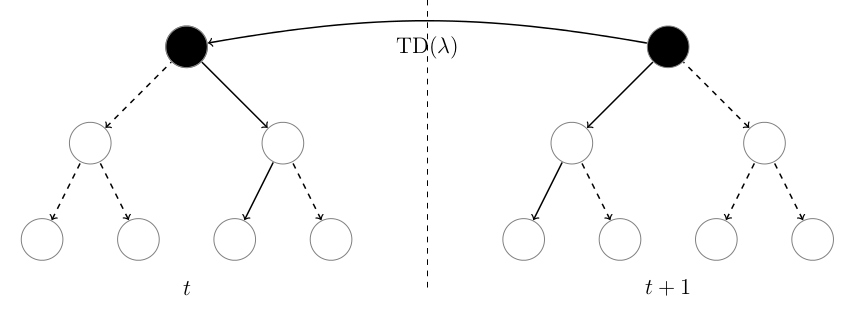
\includegraphics[scale=0.25]{tdlambda}
    \end{subfigure}
    \begin{subfigure}{0.4\textwidth}
        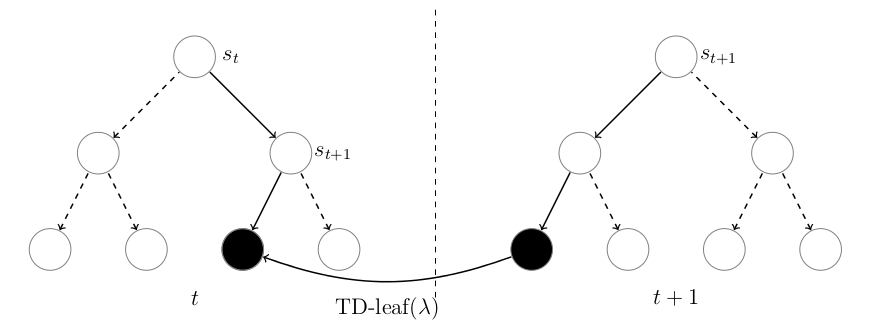
\includegraphics[trim={0.25cm 0cm 0 0cm},clip,scale=0.25]{tdl}
    \end{subfigure}
    \begin{subfigure}{0.4\textwidth}
        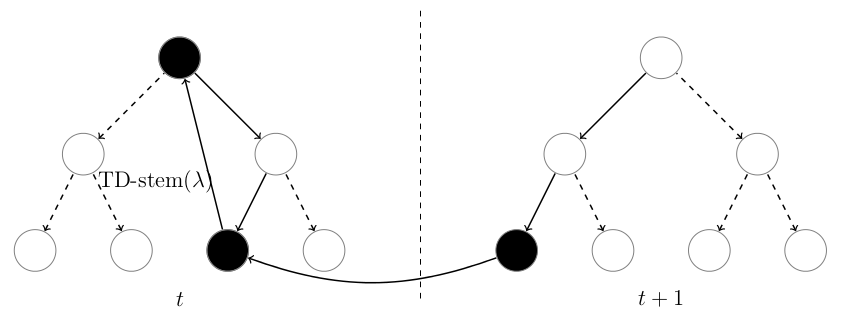
\includegraphics[trim={0cm 0cm 0.5cm 0cm},clip,scale=0.25]{tds}
    \end{subfigure}
    \caption{Comparison between the 3 discussed TD-learning algorithms, the \Gls{pv} are indicated with solid edges. In classical TD-learning the updates are between successive states. TD-leaf updates are between successive leaf nodes and in TD-stem both ideas are combined. }\label{fig:algs}
\end{figure}


\section{Network Architecture}
\label{sec:nn}
In conventional chess engines, the heuristic evaluation function is linear, but also reinforcement learning chess programs often use a linear value function \cite{knightcap,meep}. In this dissertation, we switched gears and used a neural network model instead, as they have the ability to model a larger range of functions and extract additional features from the data. Additionally, they perform quite good in practice although they do not necessarily converge under TD algorithms \cite{convergence}. Here, there has been experimented with a \gls{cnn} architecture using raw image planes as input, which is a first to our best knowledge. The activation function between all hidden units is an ordinary \gls{relu} and the weights are initialized with the tips given by Bengio et al. \cite{init}.\\

Chess boards are separated in two sets of features:
\begin{itemize}
\item bitboards: raw image planes (8x8)
\item global features: objective observations about the board 
\end{itemize}
An example of how to extract bitboards from a chess position is shown in table \ref{tab:feat}, where the chess board in figure \ref{fig:diagram} is vectorized. Feature maps are extracted from the binary image planes which are fed into a \gls{cnn}. The global features come together with a flattened version of the feature maps at the output of the final convolutional layer in a final \gls{fcn} in order to obtain the static evaluation.

\begin{figure}
\centering
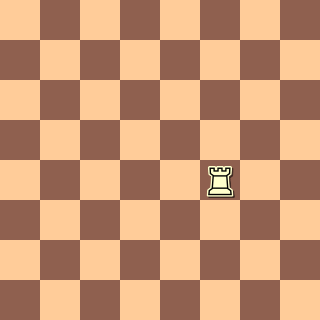
\includegraphics[scale=0.5]{diagram}
\caption{}
\label{fig:diagram}
\end{figure}

\begin{table}[]
\caption{8 Bitboards corresponding to the chess position in figure \ref{fig:diagram}. Piece maps indicate the cells where pieces reside. Mobility maps show where pieces can go to.}
\label{tab:feat}
\centering
\begin{tabular}{c c c}
\hline
\textbf{piece} & \textbf{piece map} & \textbf{mobility map}  \\
\hline
&&\\

\includegraphics[scale=0.5]{pieces/K} & 
$\begin{smallmatrix}0&0&0&0&0&0&0&0\\0&0&0&0&0&0&0&0\\0&0&0&0&1&0&0&0\\0&0&0&0&0&0&0&0\\0&0&0&0&0&0&0&0\\0&0&0&0&0&0&0&0\\0&0&0&0&0&0&0&0\\0&0&0&0&0&0&0&0\end{smallmatrix}$
&
$\begin{smallmatrix}0&0&0&0&0&0&0&0\\0&0&0&1&0&0&0&0\\0&0&0&1&0&1&0&0\\0&0&0&1&1&1&0&0\\0&0&0&0&0&0&0&0\\0&0&0&0&0&0&0&0\\0&0&0&0&0&0&0&0\\0&0&0&0&0&0&0&0\end{smallmatrix}$
\\&&\\

\includegraphics[scale=0.5]{pieces/Q} & 
$\begin{smallmatrix}0&0&0&0&0&0&0&0\\0&0&0&0&0&0&0&0\\0&0&0&0&0&0&0&0\\0&0&0&0&0&0&0&0\\0&0&0&1&0&0&0&0\\0&0&0&0&0&0&0&0\\0&0&0&0&0&0&0&0\\0&0&0&0&0&0&0&0\end{smallmatrix}$
&
$\begin{smallmatrix}0&0&0&1&0&0&0&1\\1&0&0&1&0&0&1&0\\0&1&0&1&0&1&0&0\\0&0&1&1&1&0&0&0\\1&1&1&0&1&1&1&1\\0&0&1&1&1&0&0&0\\0&1&0&1&0&1&0&0\\1&0&0&1&0&0&1&0\end{smallmatrix}$
\\&&\\

\includegraphics[scale=0.5]{pieces/k} &
$\begin{smallmatrix}0&0&0&0&0&1&0&0\\0&0&0&0&0&0&0&0\\0&0&0&0&0&0&0&0\\0&0&0&0&0&0&0&0\\0&0&0&0&0&0&0&0\\0&0&0&0&0&0&0&0\\0&0&0&0&0&0&0&0\\0&0&0&0&0&0&0&0\end{smallmatrix}$
 & 
$\begin{smallmatrix}0&0&0&0&1&0&1&0\\0&0&0&0&0&0&0&0\\0&0&0&0&0&0&0&0\\0&0&0&0&0&0&0&0\\0&0&0&0&0&0&0&0\\0&0&0&0&0&0&0&0\\0&0&0&0&0&0&0&0\\0&0&0&0&0&0&0&0\end{smallmatrix}$
\\&&\\ 
\includegraphics[scale=0.5]{pieces/q} &
$\begin{smallmatrix}0&0&0&0&0&0&0&0\\0&0&0&0&0&0&0&0\\0&0&0&0&0&0&0&0\\0&0&0&0&0&0&0&0\\0&0&0&0&0&0&0&0\\0&0&0&0&0&0&0&0\\0&0&0&0&0&0&0&0\\0&0&0&0&0&0&0&0\end{smallmatrix}$
&
$\begin{smallmatrix}0&0&0&0&0&0&0&0\\0&0&0&0&0&0&0&0\\0&0&0&0&0&0&0&0\\0&0&0&0&0&0&0&0\\0&0&0&0&0&0&0&0\\0&0&0&0&0&0&0&0\\0&0&0&0&0&0&0&0\\0&0&0&0&0&0&0&0\end{smallmatrix}$
\\&&\\
\hline
\end{tabular}
\end{table}


\section{Experiments}
\label{sec:res}
We performed two experiments on basic endgame problems by letting 2 agents with the same value function play episodes against each other starting from a random position sampled from a generated dataset and compared the final performances of TD-Leaf and TD-Stem by playing 2000 games against an optimal player making perfect moves after training. The optimality is obtained by probing a Gaviota tablebase, containing the exact \gls{dtm} and \gls{wdl} information \cite{tb}. We propose 3 metrics, the \gls{wcr}, \gls{we} and \gls{lhs} to assess the quality of a model: \textcolor{white}{Fabian}
\begin{align*}
\textnormal{WCR}&=\frac{\text{games model won}}{\text{games model should win}} \\
\textnormal{WE}&=\frac{\text{average DTM of won games}}{\text{average length of won games}}\\
\textnormal{LHS}&=\frac{\text{average length of lost games}}{\text{average DTM of lost games}}\\
\end{align*}

The complete simulation is performed through stages, which are manually controllable.
The process has been further optimized with the addition of hyper-parameters (see table \ref{tab:params_exp}), modifiable through stages. In table \ref{tab:stages} the configurations for the stages conducted in the experiments are laid out.

\begin{table}[]
\centering
\caption{Hyper-parameters modifiable in between stages.}
\label{tab:params_exp}
\begin{tabular}{rl}
\hline
$\lambda$    & Parameter for TD-learning methods                                                                                                        \\ 
$d_r$        & Depth at which immediate wins are sought                                                                                      \\ 
$d_V$        & Depth at which the value network is called                                                                                               \\ 
$f_\epsilon$ & \begin{tabular}[c]{@{}l@{}}Decay function for exploration parameter $\epsilon =f(i)$.\\  i increments every iteration.\end{tabular}      \\ 
$I$          & Number of iterations                                                                                                                     \\ 
$i_0$        & First iteration number, to initialize $\epsilon$ with the $f_\epsilon$                                                                   \\ 
$K$          & \begin{tabular}[c]{@{}l@{}}The number of states that are used to calculate the\\ $\lambda$-return from an episode\end{tabular}          \\ 
$M$          & The maximal amount of moves made in an episode                                                                                           \\ 
$N$          & How many games are played during an iteration                                                                                            \\ 
$R$          & \begin{tabular}[c]{@{}l@{}}The number of additional random moves played on the \\board position extracted from the dataset\end{tabular} \\ \hline
\end{tabular}
\end{table} 


\begin{table}[]
\centering
\caption{Hyper-parameters of the stages in the experiments}
\label{tab:stages}
\begin{tabular}{cc|rrrrrrr}
\textbf{Exp}&\textbf{Stage} & \textbf{$N$}  & \textbf{$I$} & \textbf{$d_V$} & \textbf{$\lambda$}& \textbf{$i_0$}&$K$ &$d_r$\\ \hline
& 1     & 5000 & 20  & 1     & 0.5  & 1 &  50  & 0\\
& 2     & 5000 & 20  & 1     & 0.5  & 2 &  50  & 0\\
& 3     & 5000 & 20  & 1     & 0.7  & 2 &  50  & 0\\
1 & 4     & 500  & 20  & 3     & 0.8  & 2 & 50 & 0  \\
& 5     & 250  & 30  & 3     & 0.8  & 2 &  50  & 0\\
& 6     & 250  & 30  & 3     & 0.8  & 2 &  50  & 0\\
& 7     & 250  & 50  & 3     & 0.8  & 2 &  50  & 0\\
\hline
& 1     & 500 & 20  & 1     & 0.5  & 0 & 10    & 3\\
& 2     & 250 & 20  & 3     & 0.6  & 20 & 20   & 3 \\
2 & 3     & 250 & 20  & 3     & 0.7  & 40 & 30 & 3  \\
& 4     & 250  & 50  & 3     & 0.8  & 40 & 30  & 5 \\
& 5     & 250  & 20  & 3     & 0.8  & 45 & 30  & 5 \\
\hline    
\end{tabular}
\end{table}

\begin{figure}
\centering
\begin{subfigure}{0.4\textwidth}
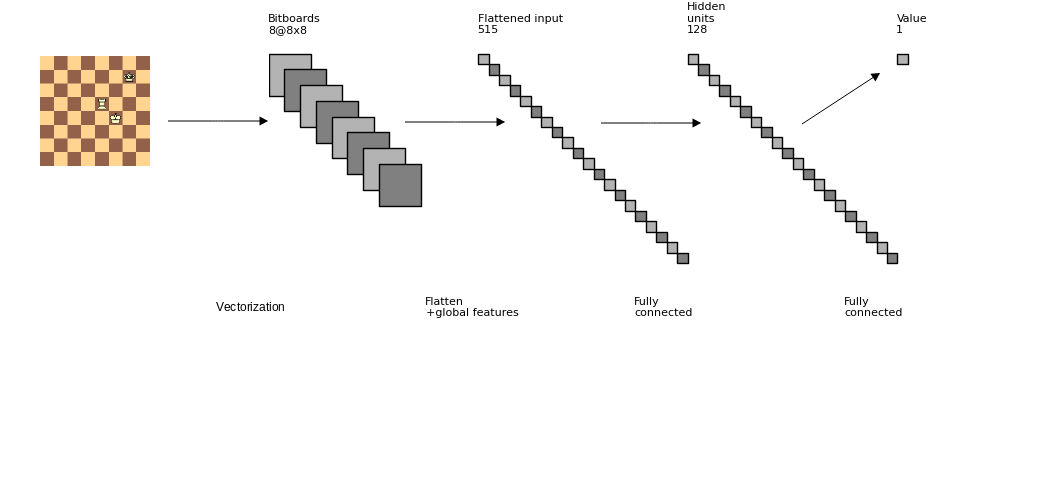
\includegraphics[trim={0 6cm 0 0cm},clip,scale=0.24]{arch/fc}
\subcaption{Depiction of the \gls{nn} used in the first experiment. The binary input features are fed into a 1 layer \gls{fnn}.}
\label{fig:fnn}
\end{subfigure}
\begin{subfigure}{0.4\textwidth}
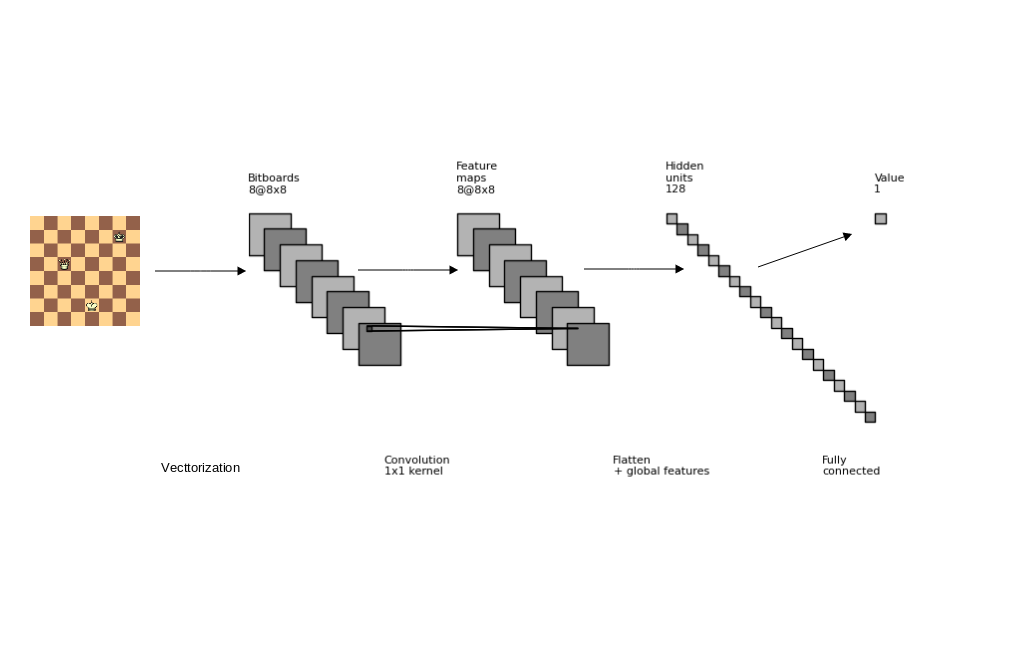
\includegraphics[trim={0 6cm 0 6cm},clip,scale=0.24]{arch/cnn1}
\subcaption{The (relatively simple) \gls{cnn} architecture deployed in experiment 2.}
\label{fig:cnn1}
\end{subfigure}
\caption{Network architectures used for the value function during the experiments.}
\end{figure}

\subsection{Experiment 1: king rook king endgame}
The first simulations we ran were on the \gls{krk} endgame, where the obvious goal for the player holding the rook is to checkmate the opponent as efficiently as possible. As only kings and rooks are set on the board, the input channels are limited to 8 bitboards. The network is trained with a learning rate of $\alpha=10^{-4}$, its architecture is represented in figure \ref{fig:fnn}. After every iteration during a stage, the exploration parameter $\epsilon$ is decreased according to the function $f_\epsilon(i)=(i)^{-3/4}$.\\
Table \ref{tab:perf_krk} confirms the hypothesis of TD-Stem being a faster learner than TD-Leaf. With the value function learned in TD-Stem, we succeed at winning about 85\% of the positions, clearly outperforming TD-Leaf. When the engine is at the losing side, it defends itself better with the novel variant.
\begin{table}[]
\centering
\caption{Performance comparison TD-Leaf($\lambda$) and TD-Stem($\lambda$),$N$ is the total number of episodes played in the simulation.}
\label{tab:perf_krk}
\begin{tabular}{l|rr}
    & \multicolumn{1}{l}{\textbf{TD-Leaf($\lambda$)}} & \multicolumn{1}{l}{ \textbf{TD-Stem($\lambda$)}} \\ \hline
\textbf{WCR} & 0.48                                   & \textbf{0.85}                          \\
\textbf{WE}  & \textbf{0.87}                          & 0.86                                   \\
\textbf{LHS} & 0.80                                   & \textbf{0.91}                          \\
\textbf{N }  & 353 500                                & \textbf{304 500}                      
\end{tabular}
\end{table}
\subsection{Experiment 2: king queen king endgame}
We try to confirm our conjecture of TD-Leaf being at least equivalent to TD-Stem in performance by analyzing an even easier problem, the \gls{kqk} endgame. The learning rate of the network depicted in figure \ref{fig:cnn1} is $\alpha=10^{-4}$. The exploration parameter $\epsilon$ obeys the decay function $f_{\epsilon}(i)=1-0.02i$.\\

A first glance at the learning curve in figure \ref{fig:lc_kqk} can trick one in believing that TD-Leaf learns quicker than TD-Stem. However, the sudden dive in the curve starting from episode 30000 corresponding with TD-Leaf hints to a contrary belief. An explanation for this behavior is that the winning rate in the plot represents the agents strength against itself, and not against the optimal agent. Hence, the decrease is a sign of an improvement at the losing side.\\
We can back this up with the observations noted in table \ref{tab:perf_kqk}, where we can see how both models still largely improve in the upcoming stages after the plateau in the learning curve is reached. Furthermore, TD-Stem plays stronger than TD-Leaf at the point in the plateau, confirming our belief of our proposal being the faster learner.\\

We provide two possible reasons why TD-Stem outperforms TD-Leaf in our experiments:
\begin{enumerate}
\item The influence of positive rewards propagates faster in updates, because depth plays a fundamental part to the learned value function at the states and their leaf nodes and so on.
\item The wrong belief effect in TD-Leaf slows down learning
\end{enumerate}
\begin{table}[]
\centering
\caption{Performance comparison TD-Leaf($\lambda$) and TD-Stem($\lambda$)}
\label{tab:perf_kqk}
\begin{tabular}{l|rr|rr}
& \multicolumn{2}{c|}{\textbf{3 stages}} & \multicolumn{2}{c}{\textbf{5 stages}} \\

    &\multicolumn{1}{l}{\small\textbf{TD-Leaf($\lambda$)}} & \multicolumn{1}{l|}{\small\textbf{TD-Stem($\lambda$)}}&\multicolumn{1}{l}{\small\textbf{TD-Leaf($\lambda$)}} & \multicolumn{1}{l}{\small\textbf{TD-Stem($\lambda$)}} \\ \hline
\textbf{WCR} & 0.65 & \textbf{0.77} & 0.90                                  & 0.90                          \\
\textbf{WE} & \textbf{0.67} & 0.64 & 0.89                          & 0.89                                   \\
\textbf{LHS} & 0.89 & 0.89 & 0.95                                   & \textbf{0.97}                          \\
\textbf{N } & \textbf{26000} & 27000  & \textbf{43500}                                & 44500                      
\end{tabular}
\end{table}

\begin{figure}
\centering
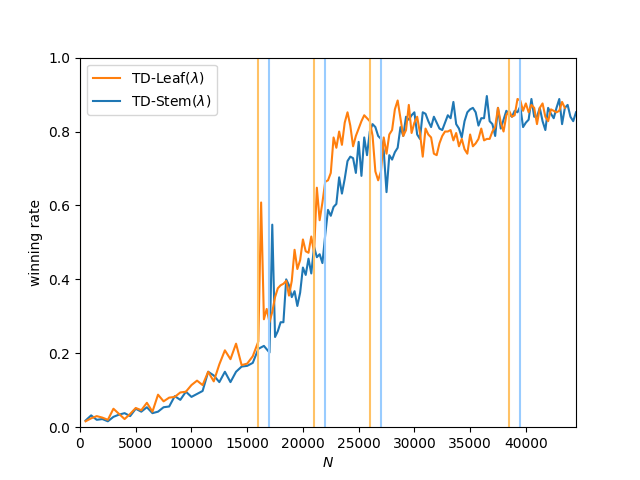
\includegraphics[scale=0.5]{plots/kqk_lc}
\caption{The learning curve of the second experiment, divided in 5 stages.}
\label{fig:lc_kqk}
\end{figure}

\section{Conclusion}
\label{sec:con}

In this study, a different approach from existing chess engines has been tried by not including any human bias to the system. To attain this property, only raw bitboard features and objective information about chess positions are fed into an \gls{nn}. The value function is learned through self play in combination with a novel \gls{rl} algorithm we called TD-Stem($\lambda$). We have compared this proposal with TD-Leaf($\lambda$) and the outcome of the experiments indicate that our variant learns faster.\\

More research can and needs to be carried out to obtain valuable knowledge about strategic game play in chess. Just as in backgammon, there might valuable positional knowledge in the game which has not been discovered yet. To explore these possibilities with \gls{rl} however, it is important to only make use of objective information (like tablebases for instance).\\

Possibilities to continue research are for example by learning on bigger endgame examples, deeper \glspl{cnn}, more bitboards extracted from chess positions and learning policy networks.

\nocite{*}
\bibliographystyle{phdsymp}
%%%%%\bibliography{bib-file}  % commented if *.bbl file included, as
%%%%%see below


%%%%%%%%%%%%%%%%% BIBLIOGRAPHY IN THE LaTeX file !!!!! %%%%%%%%%%%%%%%%%%%%%%%%
%% This is nothing else than the phdsymp_sample2e.bbl file that you would%%
%% obtain with BibTeX: you do not need to send around the *.bbl file        
%%
%%---------------------------------------------------------------------------%%
%
\begin{thebibliography}{1}
\bibitem{shannon}
Claude E. Shannon,
\newblock {\em Programming a computer for playing chess},
\newblock Philosophical Magazine, 41(314) 1950

\bibitem{turing}
Alan Turing,
\newblock {\em Chess},
\newblock Digital Computers applied to Games, 1953

\bibitem{deepblue}
Murray Campbell, Joseph Hoane Jr, Feng-hsiung Hsu 
\newblock {\em Deep Blue},
\newblock Artificial Intelligence, Vol. 134, p57-83, 2002

\bibitem{sota}
\newblock {\em CCRL 40/40 Rating List}
\newblock {\url{http://www.computerchess.org.uk/ccrl/4040/cgi/compare\_engines.cgi?print=Rating+list+%28text%29&class=all+engines&only_best_in_class=1}}
\newblock 2017

\bibitem{samuel}
Arthur L. Samuel 
\newblock {\em Some Studies in Machine Learning Using the Game of Checkers},
\newblock {IBM} Journal of Research and Development, Vol. 3, p210-229, 1959

\bibitem{tesauro}
Gerald Tesauro
\newblock {\em Temporal Difference Learning and TD-Gammon},
\newblock Communications of the ACM, Vol. 38, p58-68, 1995

\bibitem{knightcap}
Jonathan Baxter, Andrew Tridgell and Lex Weaver
\newblock {\em TDLeaf(lambda): Combining Temporal Difference Learning with Game-Tree Search},
\newblock CoRR, 1999

\bibitem{giraffe}
Matthew Lai
\newblock {\em Giraffe: Using Deep Reinforcement Learning to Play Chess},
\newblock diploma thesis Imperial College London, 2015

\bibitem{meep}
Joel Veness, David Silver, Alan Blair and William Uther
\newblock {\em Bootstrapping from Game Tree Search},
\newblock Advances in Neural Information Processing System Vol. 22 p.1937-1945, 2009

\bibitem{deepchess}
Omid E. David, Nathan S. Netanyahu, Lior Wolf
\newblock {\em DeepChess: End-to-End Deep Neural Network for Automatic Learning in Chess},
\newblock Artificial Neural Networks and Machine Learning – ICANN 2016

\bibitem{atari}
Volodymyr Mnih, Koray Kavukcuoglu, David Silver, Alex Graves, Ioannis Antonoglou, Daan Wierstra and Martin Riedmiller
\newblock {\em Playing Atari with Deep Reinforcement Learning},
\newblock NIPS Deep Learning Workshop 2013

\bibitem{dddqn}
Ziyu Wang, Nando de Freitas and Marc Lanctot
\newblock {\em Dueling Network Architectures for Deep Reinforcement Learning},
\newblock CoRR 2015

\bibitem{alphago}
David Silver, Aja Huang, Chris J. Madison et al.
\newblock {\em Mastering the game of Go with deep neural networks and tree search},
\newblock Nature Vol. 529 p484-489, 2016


\bibitem{rl}
Richard S. Sutton and Andrew G. Barton,
\newblock {\em Introduction to Reinforcement Learning},
\newblock 1998

\bibitem{alphabeta}
George T. Heineman, Gary Pollice andStanley Selkow (2008),
\newblock {\em Algorithms in a Nutshell},
\newblock p217–223, 1998

\bibitem{rlalg}
Csaba Szepesv{\'a}ri
\newblock {\em Algorithms for Reinforcement Learning},
\newblock 2010

\bibitem{convergence}
J.N. Tsitsikilis, B.V. Roy 
\newblock{\em An Analysis of Temporal Difference Learning with Function Approximation }
\newblock IEEE Transactions on Automatic Control, Vol.42(5), p674–690 1996

\bibitem{tb}
Galen Huntington, Guy Haworth, 
\newblock{\em Depth to Mate and the 50-Move Rule.}
\newblock ICGA Journal, Vol. 38, No. 2

\bibitem{init}
Xavier Glorot, Yoshua Bengio
\newblock{\em Understanding the difficulty of training deep feedforward neural networks}
\newblock Proceedings of the Thirteenth International Conference on Artificial Intelligence and Statistics, PMLR 9: p249-256, 2010

\end{thebibliography}
%
%%---------------------------------------------------------------------------%%



\end{document}

%%%%%%%%%%%%%%%%%%%%%  End of phdsymp_sample2e.tex  %%%%%%%%%%%%%%%%%%%%%%%%%%%


\setlength{\voffset}{0cm}
\setlength{\hoffset}{0cm}

%\addcontentsline{toc}{chapter}{Abstract}
%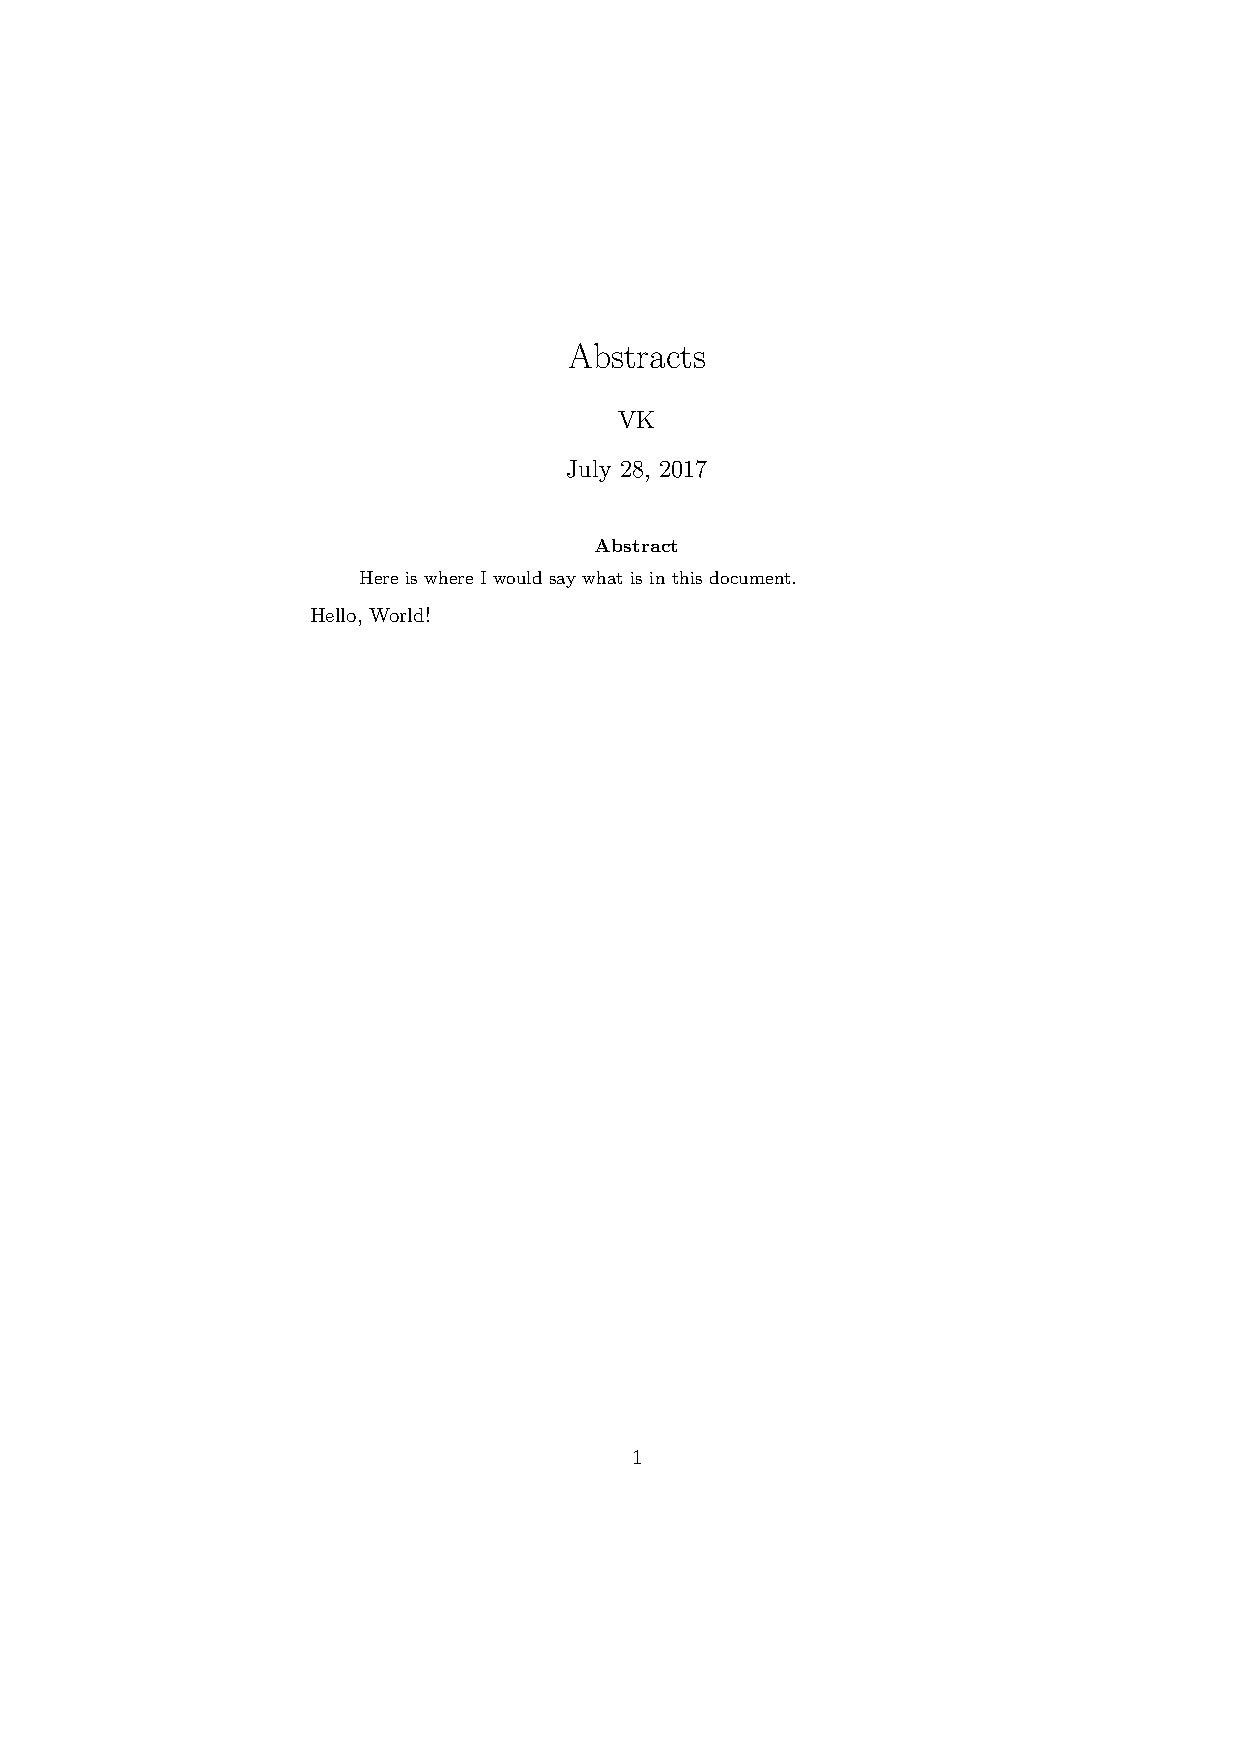
\includepdf[pages=-]{abstract.pdf}
\addcontentsline{toc}{chapter}{Extended abstract}
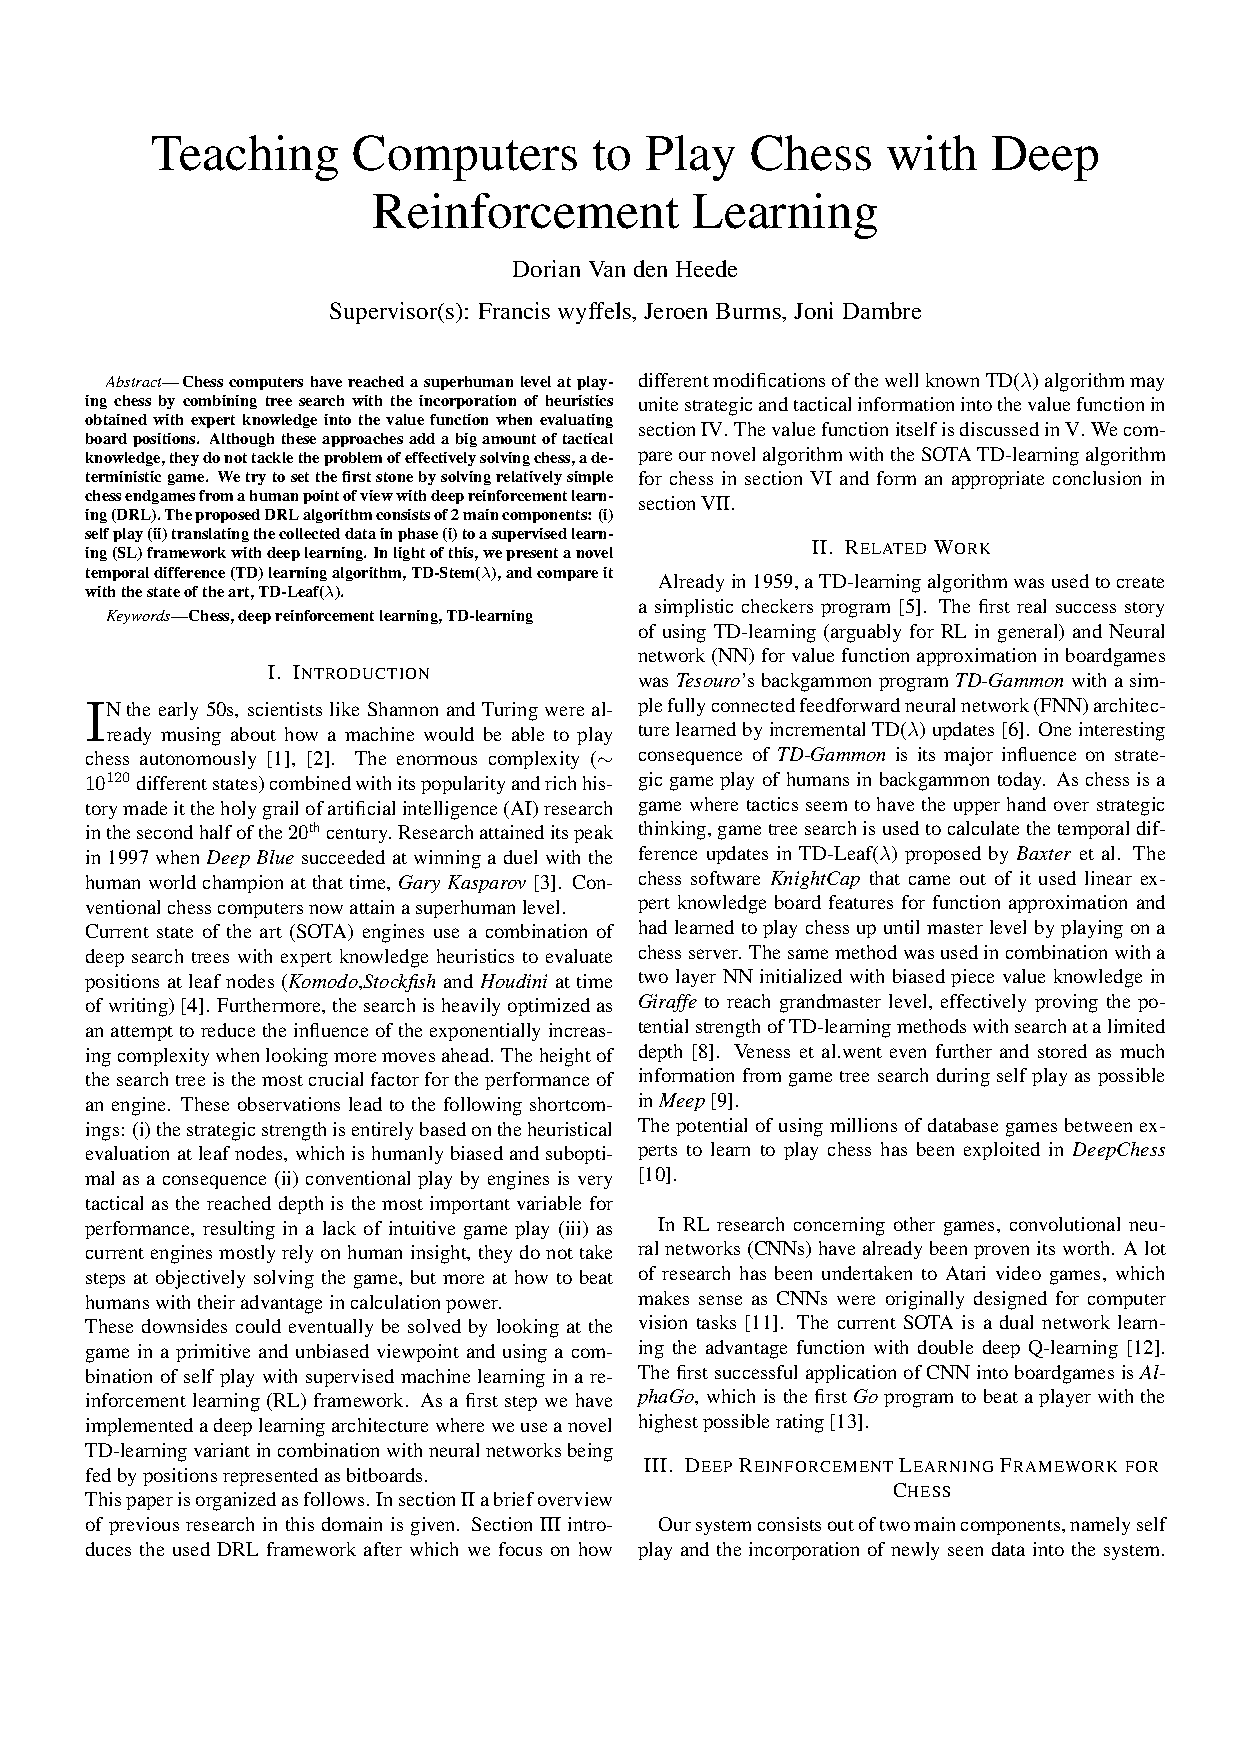
\includepdf[pages=-,width=\textwidth]{abstracts/abstract.pdf}

\setlength{\voffset}{-1in}
\setlength{\hoffset}{-1in}


% inhoudstafel
\tableofcontents

\newpage
\addcontentsline{toc}{chapter}{List of Figures}
\listoffigures
\newpage
\addcontentsline{toc}{chapter}{List of Tables}
\listoftables
\newpage
\addcontentsline{toc}{chapter}{List of Algorithms}
\listofalgorithms

\glsaddall
\printglossary[type=\acronymtype]

% opmaak voor het eigenlijke boek; onderstaande lijnen
% weglaten als de eerste regel van een nieuwe alinea moet
% inspringen in plaats van extra tussenruimte
%\setlength{\parindent}{0pt}
%\setlength{\parskip}{0.5\baselineskip plus 0.5ex minus 0.2ex}
%\setlength{\parskip}{1ex plus 0.5ex minus 0.2ex}

% hoofdstukken
\mainmatter

% hier worden de hoofdstukken ingevoegd (\includes)
\chapter{Introduction}

Ever since computer science started to emerge as a proper field, researchers have been attracted to the problem of letting computers play the game of chess. This is mainly out of theoretical interest for \gls{ai}, as it is a human task. Chess is a complex game (it has been estimated that around $10^{120}$ unique board positions exist \cite{shann50}), which makes brute force algorithms completely unscalable. In the early 50's, notable scientists such as Turing and Shannon created a theoretical chess program on paper \cite{shann50,tur53}. Remarkable is they both already included the notions of an evaluation function, minimax and quiescent search. These concepts are still used today in state of the art chess programs. \\

In the second half of the 20th century, computer chess evolved further and further. Continuous minor adjustments were made to the heuristics of the evaluation function, computation became more and more parallelized and search methods were improved with more efficient pruning. This led to the victory of \textit{Deep Blue} against world champion at that time Gary Kasparov in 1997 \cite{dblue02}, an event that received a lot of attention from the media, mainly due to the symbolical significance of machine catching up with human intelligence \cite{wstd97}. \\

Since that event, computer chess was studied less and less and the \textit{Drosophila} \footnote{Drosophila species are extensively used as model organisms in genetics for testing new techniques. It is used as a metaphor in this context.} of \gls{ai} research became go, a game that is, despite its simplicity of rules, extremely complex. Search techniques classically used in chess engines are less usable for go engines mainly due to the size of the board and large amount of possible moves every ply. Recently in 2016, a \textit{Google} research team succeeded at beating a 9-dan \footnote{Highest rating achievable in \textit{go}.} professional player \cite{alphago16}. The researchers achieved this by using a combination of tree search algorithms and deep \gls{rl}. This success lead to a nomination by \textit{Science} magazine for \textit{Breaktrough of the Year} \cite{scboy16}. \\

In this master thesis, we look into how \acrlong{rl} and other \acrlong{ml} techniques could be used on chess as well. Through self play and deep neural networks for the evaluation function we investigate what machines can learn about the chess game without any prior knowledge except the rules. This lack of inserting human knowledge into the system makes the learning agent as unbiased as possible, which is necessary to truly reveal the power of \gls{rl}. In a similar manner by a huge amount of stochastic self play combined with a TD learning algorithm \footnote{A \gls{rl} algorithm, further discussed in chapter \ref{ch:background}}, \textit{TD-gammon} was able to discover new strategies humans never thought about before \cite{tdgammon95}.\\

The move decision of current chess computers is based on looking ahead as far as possible. They build a game tree and evaluate positions at the bottom of the tree with a static evaluation function. The move choice is then the one that would lead to the best evaluation at the bottom of the tree under the assumption that both players try to make the best moves. the search is heavily optimized as an attempt to reduce the influence of the exponentially increasing complexity when looking more moves ahead. The height of the search tree is the most crucial factor for the performance of an engine.\\

The evaluation function is usually a heuristic based where game technical knowledge is used, which has been gathered during the history of the game by expert chess players. These rules are not objective, as they were determined by humans. On top of that, chess computers have difficulties at playing intuitively.. They still show signs of weakness in the endgame, and it takes a lot of effort to design or improve them. Furthermore, porting these technique to other games requires redesigning most of the heuristics, and the resulting \glspl{ai} do not always achieve a similar high level of play for more strategical games.\\

All current machine learning approaches to learn the static evaluation function use the helping hand of human knowledge about the chess game in their learning system. This makes it harder to actually improve on the classical state of the art approaches with heuristics. The purpose of this thesis is to research how a machine could teach itself to play chess with the rules as only knowledge. Choosing for a completely unbiased system could make the chess engine learn strategies humans never thought about before, just like what happened with \textit{TD-Gammon}. \\

There have been recent and less recent efforts to incorporate machine learning into chess engines. Recently in 2015, an end-to-end machine learning chess engine incorporating self play and reinforcement learning has reached the FIDE International Master level, while Grandmaster level can be achieved with the use of millions of database games \cite{giraffe15,deepchess16}. \\

Deep \gls{rl} can help us out with our quest at perfecting chess play and strategy. In \gls{rl}, agents are released in an environment where they have to find out by exploration which actions generate the best cumulative rewards. To improve their play, the agents make use of the gained experience. In this case, the board is the environment and white and black are the agents. By only incorporating basic and objective game elements into the framework the agents can discover by themselves what is good and what not, without additional biased knowledge. By using self play in a Deep \gls{rl} framework a value function can be constructed with only information observed by the agents themselves. As this would all be learned by the agents experience, the final static evaluation could introduce additional depth information, making deeper searches less necessary. \\
%TODO:kort overzicht sota van huidige chess engines (hoe werken ze ongeveer)
%TODO:redenen/motivatie waarom rl hierbij kan helpen


%TODO eventueel iets meer sota ivm deep rl (vb atari)
Deep \gls{rl} has already proven its worth in games, \textit{Atari} and \textit{Go} being most noteworthy. The fact that sensory image data is being processed during playing \textit{Atari} games made it the first game where \glspl{cnn} were proven successful \cite{silv13}. These video games are an excellent toy to mess around and experiment with new deep \gls{rl} algorithms. \gls{ai} game play on \textit{Atari} games has evolved further and new architectures came along the way \cite{dddqn15}.\\

In this master's thesis we will set the first step in the quest to let machines master the complete chess game through self play only and gaining experience without biased supervision. More specifically, we introduce new algorithms that can be used along the way. Due to time constraints and complexity of the overall problem, it has not been possible to implement and examine all covered techniques, but we compare a new \gls{td} learning algorithm, TD-Stem($\lambda$), with a state of the art mechanism to improve chess play with \gls{rl}. We also limit ourselves to easy chess endgame problems, as they give the opportunity for objective quality assessments. The learned models could be used to learn more complex chess positions as well from the bottom up.\\
The main questions we try to answer in this dissertation are:
\begin{itemize}
\item How would one program a chess engine without bias with deep \gls{rl}?
\item What is the best TD learning algorithm for this cause?
\end{itemize}

This book is organized as follows. We start off in chapter \ref{ch:background} by exploring how current chess computers achieve their strength and further discuss the remaining weaknesses. In chapter \ref{ch:background} an overview is given of deep learning. The knowledge gained in these two chapters are combined in chapter \ref{ch:drlgames}, where existing and new ideas are combined to propose possible architectures and techniques for programming a chess computer with deep \gls{rl}. The setup of the carried out experiments are further discussed in chapter \ref{ch:experiments}. Subsequently, the results of these experiments are presented and discussed in chapter \ref{ch:res}. This thesis is finalized in a conclusion in chapter \ref{ch:conclusion}.

For the readers whom are less familiar with the game of chess, we provide a brief introduction in appendix \ref{ch:chess_app}.








\chapter{Conventional Chess Engines}
\label{ch:chess}

State of the art chess computers search into a tree which is branched by the possible moves the players can make. The chosen move is then the move where the most plausible leaf in the tree yields the highest evaluation. Most engines choose to set up this evaluation heuristically, using expert knowledge. Tree search is computationally speaking a very complex operation, which is why branches are pruned as much as possible and heuristics are kept simple to provide fast evaluations. Generally speaking, due to the very time consuming calculations, code is optimized intensively. These optimizations happen in software as well in hardware. To gain computer power, the engines take up most of the CPUs when possible to branch through the search tree, as these operations are highly parallelizable. \\ 
In this chapter, we will look at the principal techniques used in current chess engines. These methods are typically optimized as much as possible to reduce computational overhead. This chapter is divided into four sections, each one describing an important aspect about the determination of the value function of the current board position. This value function is the mapping of a chess board to a score to indicate which side has the best chances. These methods can give an insight in how to improve Deep RL algorithms with respect to chess.\\
First, we will look at how the size of the search tree of possible future moves is reduced in section \ref{sec:search}. Next we consider how to evaluate a board position in section \ref{sec:evaluation}, after which we conclude the chapter by looking into how we can use data intensive knowledge to improve play in section \ref{sec:databases}.

\section{Search}
\label{sec:search}
Due to the tactical nature of chess (i.e. every slightest modification in board configuration can drastically change the evaluation), it seems to be nearly impossible to find an algorithm generating the best move in a blink of an eye. This is why some lookahead is needed to evaluate positions reliably. The search to the best move is done by branching through a tree structure where edges represent moves, and the nodes connected by the edges the positions before and after the move. An example of a search tree is depicted in \ref{fig:searchtree}. \\
One problem is that the search tree grows exponentially for every move made. Suppose we want to look at a depth $d$ (the lateral length of the tree, in this context the maximal number of moves thought ahead) and we can make on average the branching factor $b$ moves every ply, the size of the search tree is $b^{d}$. As chess' branching factor is around 35 \cite{levin14}, the depth is limited very rapidly. At the same time, the deeper an engine can look ahead, the stronger it plays. This is why researchers try to reduce as many branches in the search tree as possible.

%\begin{figure}
%\centering
%\begin{tikzpicture}
%\node[] (root) at (0,0) {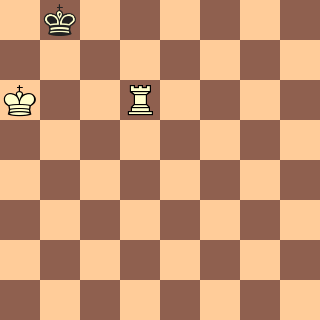
\includegraphics[width=0.1\textwidth]{fig/search/3}};
%%\draw (-)
%
%\node[] at (-1.5,-3) {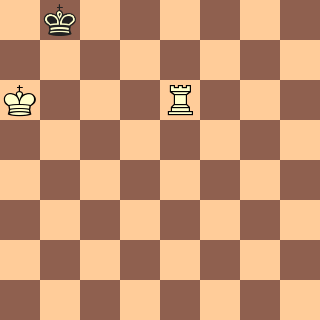
\includegraphics[width=0.1\textwidth]{fig/search/5}};
%\node[] at (-4.5,-3) {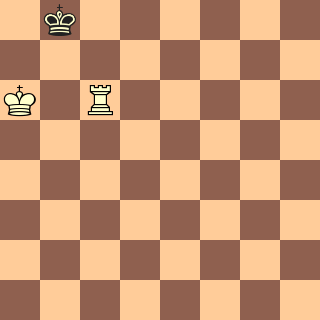
\includegraphics[width=0.1\textwidth]{fig/search/2}};
%\node[] at (4.5,-3) {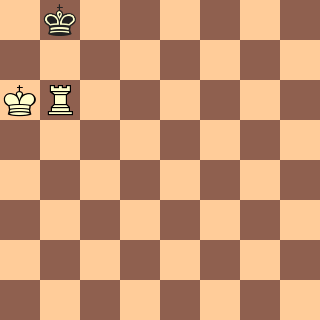
\includegraphics[width=0.1\textwidth]{fig/search/1}};
%\node at (1.5,-3) {$\cdots$};
%
%\node[] at (-4.5,-6) {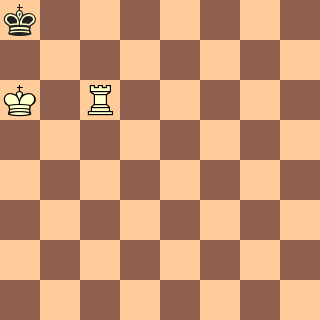
\includegraphics[width=0.1\textwidth]{fig/search/4}};
%\node[] at (2.2,-6) {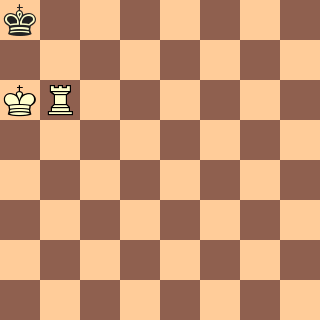
\includegraphics[width=0.1\textwidth]{fig/search/8}};
%\node[] at (6.8,-6) {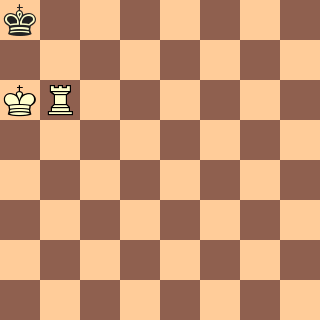
\includegraphics[width=0.1\textwidth]{fig/search/8}};
%
%\node[] at (-4.5,-9) {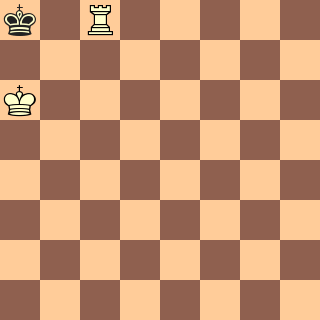
\includegraphics[width=0.1\textwidth]{fig/search/6}};
%\end{tikzpicture}
%\end{figure}

\begin{figure}
\centering
\begin{tikzpicture}[
%level 1/.style={sibling distance=30mm,level distance=3cm},level 2/.style={sibling distance=10mm},level 3/.style={sibling distance=10mm},first/.style={level distance=3cm},
%  second/.style={level distance=3cm,sibling distance=30mm},
%  third/.style={level distance=3cm,sibling distance=30mm},
%  rect/.style={rectangle,minimum size=0.15\textwidth,anchor=south}
	level distance=30mm,
	sibling distance=30mm
  ]
  \tikzstyle{every node}=[rectangle,minimum size=0.15\textwidth]
  
  \node[] {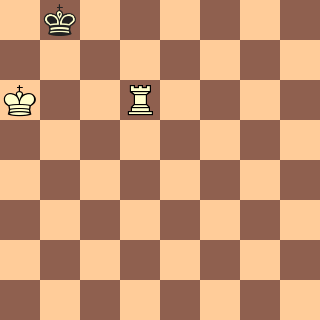
\includegraphics[width=0.15\textwidth]{fig/search/3}} [edge from parent fork down]
  	child{ node[] {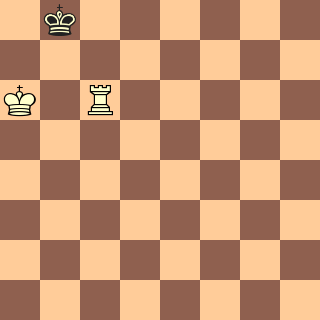
\includegraphics[width=0.15\textwidth]{fig/search/2}}
    		child{node[] {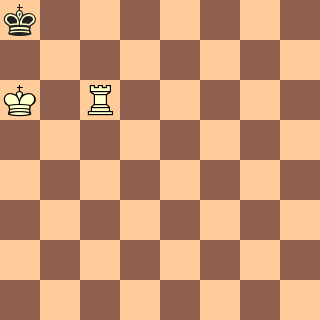
\includegraphics[width=0.15\textwidth]{fig/search/4}}
    			child{node {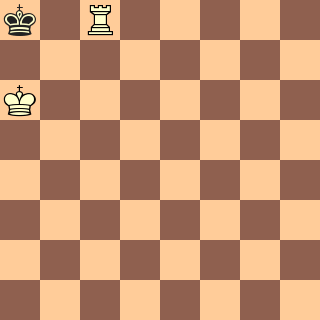
\includegraphics[width=0.15\textwidth]{fig/search/6}}}
    			child{node {$\cdots$}}
    			}
    		}
  	child{ node[] {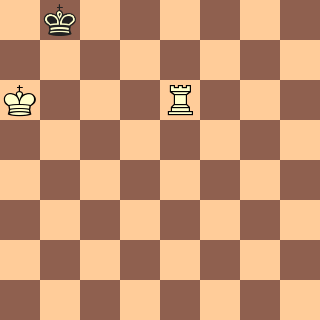
\includegraphics[width=0.15\textwidth]{fig/search/5}}
  		child{node {$\cdots$}}
  		}
  	child{ node[] {$\cdots$}}
  	child{ node[] {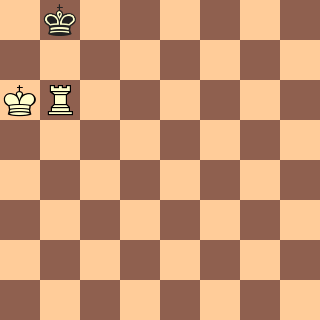
\includegraphics[width=0.15\textwidth]{fig/search/1}}
  		child{node[] {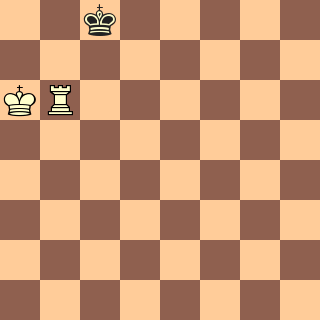
\includegraphics[width=0.15\textwidth]{fig/search/7}}}
  		child{node[] {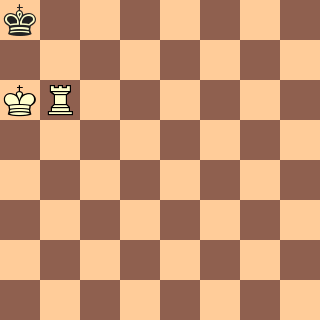
\includegraphics[width=0.15\textwidth]{fig/search/8}}}
  		child{node[] {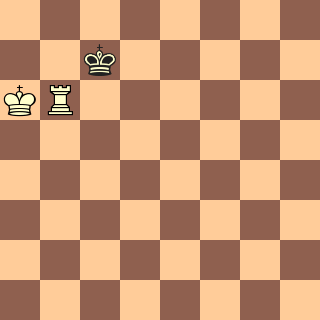
\includegraphics[width=0.15\textwidth]{fig/search/9}}}
  		};

\end{tikzpicture}
\caption[Search tree]{An illustration of a search tree up to $d=3$.}
\label{fig:searchtree}
\end{figure}

\subsection{Minimax}
\label{subsec:minimax}
Minimax is the algorithm describing how to evaluate the root position given the static evaluations of the leaf positions in games. Basically, when we look deeper into the tree, we have to alternately choose between the score of whites and blacks best move. In game theory terminology white and black are called the max-player and min-player, respectively. As the name suggests, the max-player tries to maximize the score while the min-player tries to minimize it. Due to the simplicity of zero-sum games like chess (they are symmetrical, both players try to achieve exactly the same goal, namely checkmating the opponent), the evaluation of a position is equivalent to the negation of the evaluation from the opponent's viewpoint:

\begin{equation}
V^{(w)}(s)\equiv -V^{(b)}(s)
\label{eq:zerosum}
\end{equation}

with $V^{(w)}(s)$ and $V^{(b)}(s)$ the value functions from white and blacks point of view respectively. Value functions indicate the expected outcome of position (an estimated or exact score appropriate to the position).
If one side is winning, the other one is losing. This simplification of minimax with the zero-sum property (also called negamax in literature) is listed as pseudo code in algorithm \ref{al:minimax}.

\begin{algorithm}
  \caption{Minimax}
  \label{al:minimax}
  \begin{algorithmic}
  \REQUIRE board, depth
  \ENSURE  max \\
  \COMMENT{max-player should call \textit{Minimax}(board,depth)} \\
  \COMMENT{first call min-player should be -\textit{Minimax}(board,depth)}
  \IF {depth $\leftarrow 0$}
  \RETURN \textit{Evaluation}(board) 
  \COMMENT{static evaluation of a leaf node}
  \ENDIF

  \STATE max $\leftarrow -\inf$ 
  \FOR{move \textbf{in} \textit{LegalMoves}(board)}
  \STATE newboard $\leftarrow doMove$(board, move)
  \STATE score $\leftarrow -Minimax$(newboard, depth - 1)
  \IF {score $>$ max}
  \STATE max $\leftarrow$ score
  \ENDIF
  \ENDFOR
  \RETURN max
  \end{algorithmic}
\end{algorithm}


\subsection{$\alpha \beta$-pruning}
\label{subsec:alphabeta}
Minimax requires traversing the entire search tree, which is not at all feasible as explained before due to the exponential growth of the search tree. Luckily, an improvement can be made to minimax which allows to safely prune certain subtrees. This improvement is called $\alpha \beta$-pruning, and was already proposed in 1955 \cite{mccarthy55}. The number of nodes to be evaluated is reduced by not traversing nodes further in a branch-and-bound manner when a refutation has been found. In the (recursive) algorithm, two values are stored: $\alpha$ and $\beta$. $\alpha$ represents the minimal score for the max-player in a variation, while $\beta$ represents the maximal score for the min-player. In other words, they are the provisional worst case scenario evaluations for both parties. Based on $\alpha$ and $\beta$, variations can be cut off if proven to involve inferior game play by one of the players. A formal algorithm for games with the zero-sum property is provided in algorithm \ref{al:alphabeta}. Completely worked out examples enhance the understanding significantly, therefore we encourage the reader to look at the cited website \cite{abpractice}. \\
In the worst case, we always evaluate bad leafs and end up with the same complexity of minimax, $O(b^d)$. In the best case scenario, edges corresponding with good moves are traversed first, resulting in hard to beat $\alpha$ and $\beta$ values. By always choosing to branch through the best moves in the search tree we achieve the square root of the original time complexity of minimax $O(b^{\frac{d}{2}})$ \cite{stuart2003}. From this reasoning, it follows that the move ordering of branching is very important, as we could potentially gain twice the depth in our search in the same timespan (see table \ref{tab:alphabeta} for a comparison). Heuristics as well as machine learning techniques like \acrlong{nn}s can be used to determine the move order of the search \cite{hashmoveorder05,nnmovemap02}.

\begin{algorithm}
\caption{$\alpha \beta$Minimax}
\label{al:alphabeta}
\begin{algorithmic}[]
\REQUIRE board, depth, $\alpha$, $\beta$
\ENSURE $\alpha$\\
\COMMENT{max-player should call \textit{Minimax}(board,depthLeft,$-\infty$,$\infty$)} \\
\COMMENT{min-player should call -\textit{Minimax}(board,depthLeft,$-\infty$,$\infty$)}
\IF {depthLeft $\leftarrow 0$}
\RETURN \textit{Evaluation}(board) 
\COMMENT{static evaluation of a leaf node}
\ENDIF
\FOR{move \textbf{in} \textit{LegalMoves}(board)}
\STATE newboard $\leftarrow doMove$(board, move)
\STATE score $\leftarrow -\alpha \beta Minimax$(newboard, depthLeft - 1,$-\beta$,$-\alpha$)
\COMMENT{Exchanging because of zero-sum property}
\IF{score $\geq \beta$}
\RETURN $\beta$
\COMMENT{$\beta$-cutoff}
\ENDIF
\IF{score $> \alpha$}
\STATE{$\alpha \leftarrow$ score}
\COMMENT{$\alpha$ is the max from \textit{Minimax (Algorithm \ref{al:minimax})}}
\ENDIF
\ENDFOR
\RETURN $\alpha$
\end{algorithmic}
\end{algorithm}

\begin{table}[]
\centering
\caption[Comparison $\alpha\beta$-pruning and regular minimax]{The exact number of explored nodes in the best case scenario is $b^{\lceil \frac{d}{2} \rceil}+b^{\lfloor \frac{d}{2} \rfloor}-1 $ \cite{edw61}, while it is $b^{d}$ in regular minimax, which is the worst case for $\alpha \beta$-pruning.}
\label{tab:alphabeta}
\begin{tabular}{rrr}
\toprule
\textbf{depth} & \textbf{worst case} & \textbf{best case} \\
\midrule
0              & $1 \cdot 10^0$                   & $1\cdot 10^0$                  \\
1              & $3.5\cdot 10^1$                & $3.5\cdot 10^1$                 \\
2              & $1.225\cdot 10^3$                & $6.9\cdot 10^1$                 \\
3              & $4.287 \cdot 10^4$  			& $1.259\cdot 10^3$               \\
4              & $1.500\cdot 10^6$             & $2.449\cdot 10^3$               \\
5              & $5.252\cdot 10^7$            & $4.409\cdot 10^4$              \\
6              & $1.838\cdot 10^9$          & $8.574\cdot 10^4$              \\
7              & $6.433\cdot 10^{10}$         & $1.543\cdot 10^6$            \\
8              & $2.251\cdot 10^{12}$       & $3.001\cdot 10^6$            \\
9              & $7.881\cdot 10^{13}$      & $5.402\cdot 10^7$           \\
10             & $2.758\cdot 10^{15}$    & $1.050\cdot 10^8$          \\
\bottomrule
\end{tabular}
\end{table}

\subsection{Principal Variation Search}
\label{subsec:pvs}
\glspl{pvs} (which in literature is often put equal to the almost identical \textit{negascout} algorithm) is a further improvement to the $\alpha \beta$-pruning minimax algorithm which in general leads to a save in computation time when the move ordering is done right. \\ 
The idea is the following: we base our calculations on the principal variation, which is the path in the tree corresponding to the intuitively best move (this could be calculated for example with shallow searches of limited depth). The first node typically traversed is part of the principal variation, after which we continue with regular $\alpha \beta$-pruning. For all the other moves, we set up a small window based (i.e. we suppose $\beta$ to be close to $\alpha$) on the $\alpha$-value found in the principal variation. The immediate consequence is a growing number of $\beta$-cutoffs. If we were to find a variation leading to a score in the window, we know our initial assumption was wrong, and we have to search through the same node once more with general $\alpha \beta$-pruning. This is why the move ordering is crucial for this to work. See algorithm \ref{al:pvs} for pseudo code.\\
\gls{pvs} and negascout yield the same result as $\alpha \beta$-pruning \cite{reine89}. The algorithm is heavily based on the original \textit{Scout} algorithm, which was the first algorithm to outperform $\alpha \beta$-pruning \cite{pearl80}. \\

Another minimax search algorithm has been implemented, proven to outperform \gls{pvs} and negascout in practice, namely \textit{MTD(f)} \cite{plaat96}. The window calls from \gls{pvs} only return a bound on the minimax value. In contrast, MTD(f) calls a full $\alpha \beta$-search a number of times, converging towards the exact value. Overhead of searching through the same nodes is covered by transition tables in memory.

\begin{algorithm}
\caption{PVS}
\label{al:pvs}
\begin{algorithmic}[]
\REQUIRE board, depth, $\alpha$, $\beta$
\ENSURE max \\
\COMMENT{max-player should call \textit{PVS}(board,depth,$-\infty$,$\infty$)} \\
\COMMENT{min-player should call -\textit{PVS}(board,depth,$-\infty$,$\infty$)}
\IF {depth $\leftarrow 0$}
\RETURN \textit{Evaluation}(board) 
\ENDIF \\
\COMMENT{First, calculate score of principal variation with full $\alpha \beta$-search}
\STATE pv $\leftarrow$ \textit{PV}(board)
\STATE newboard $\leftarrow doMove$(board, pv)
\STATE $\alpha \leftarrow$ -\textit{PVS}(newboard,depth$-1$,$-\beta$,$-\alpha$) \\
\COMMENT{Look at other moves in a reduced window $[ \alpha,\alpha +1]$ \cite{fishburn84}}
\FOR{move \textbf{in} \textit{LegalMoves}(board) \textbf{and} move $\neq$ pv}
\STATE newboard $\leftarrow doMove$(board, move)
\STATE score $\leftarrow -PVS$(newboard, depth - 1,$-\alpha-1$,$-\alpha$)
\IF{$\alpha < $score$ < \beta$}
\STATE score $\leftarrow -PVS$(newboard, depth - 1,$\beta$,$-\alpha$)
\COMMENT{Wrong guess of pv, full research}
\ENDIF
\IF{score $\geq \beta$}
\RETURN $\beta$
\COMMENT{$\beta$-cutoff}
\ENDIF
\IF{score $> \alpha$}
\STATE{$\alpha \leftarrow$ score}
\ENDIF
\ENDFOR
\RETURN $\alpha$
\end{algorithmic}
\end{algorithm}

\subsection{Quiescence Search}
\label{subsec:qs}
A remaining problem after the already presented search algorithms is the fixed depth. This can cause the horizon effect, the evaluation at the leaf node can be suboptimal due to the possible presence of tactical moves completely changing the static evaluation. An example of how problematic this can be is shown in figure \ref{fig:qs}. \\
Typical tactical moves that are considered are piece captures and checks. The search goes on until the node seems 'quiet' enough, or by finding a new lower bound to the minimax score with a static evaluation \cite{beal90}. This enhancement is based on the null move observation, which expresses that it is (almost \footnote{In rare cases, no good moves are available, and a player is forced to weaken its position. These positions are called zugzwang positions}) always better for the side to move to play than to do nothing.

\begin{figure}
    \centering
    \begin{subfigure}[b]{0.3\textwidth}
        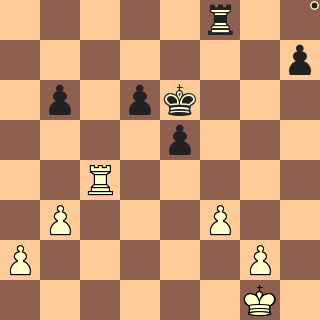
\includegraphics[width=\textwidth]{fig/diagram_qs_1}
        \caption{Black to move}
        \label{fig:qs1}
    \end{subfigure}
    ~ %add desired spacing between images, e. g. ~, \quad, \qquad, \hfill etc. 
      %(or a blank line to force the subfigure onto a new line)
    \begin{subfigure}[b]{0.3\textwidth}
        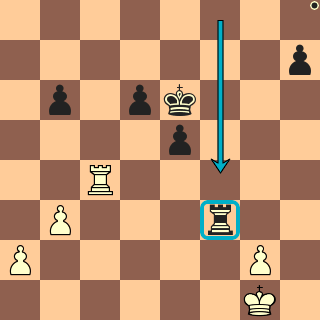
\includegraphics[width=\textwidth]{fig/diagram_qs_2}
        \caption{White to move}
        \label{fig:qs2}
    \end{subfigure}
    ~ %add desired spacing between images, e. g. ~, \quad, \qquad, \hfill etc. 
    %(or a blank line to force the subfigure onto a new line)
    \begin{subfigure}[b]{0.3\textwidth}
        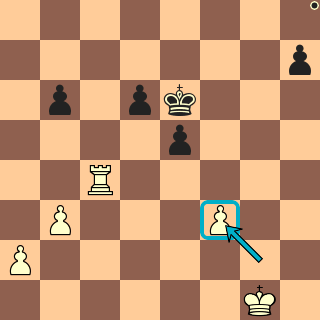
\includegraphics[width=\textwidth]{fig/diagram_qs_3}
        \caption{Black to move}
        \label{fig:qs3}
    \end{subfigure}
    \caption[Importance quiescence search]{Suppose the remaining depth after figure \ref{fig:qs2} is 0, then a static evaluation of the position is required. Without any \gls{qs}, a typical engine would first of all count all the pieces on the board and note that black is a pawn up, hence yield an evaluation in favor of black. This is utterly wrong, as white is winning in this position, due to the tactical change at the next move gxf3. Now White is a Rook up in exchange of a pawn. The figure \ref{fig:qs3} shows the resulting position after the exchange. There are no remaining tactical threats in this position, hence this is a quiet position. The engine should have computed this as well to provide a reliable minimax evaluation.}
    \label{fig:qs}
\end{figure}

\subsection{Other Search Improvements}
\label{subsec:others}
In this subsection, we briefly discuss other possible (some of them obligatory) enhancements to regular $\alpha \beta$-search. \\

While traversing through the search tree, stakes are high chess engines encounter the same states again and again (but achieved through different paths). This is why a transposition table is stored in memory, which is essentially a large hash table storing information about all encountered positions \cite{kishimoto02}. Typical characteristics that are stored in an entry are
\begin{itemize}
\item best move
\item highest calculated depth
\item score
\end{itemize}

Another almost obligatory enhancement on the basic methodology is iterative deepening. Because of the exponential complexity and uncertainty about the duration of searching (e.g. in \gls{qs}), time management is required. Some time is allocated for the search of a best move, and systematically the calculations go deeper and deeper. In case of time running out, the engine can still fall back to the best move according to current calculations, this as opposed to to depth first searches. Usually, the depth first algorithms like $\alpha \beta$-pruning (as we have seen in previous sections) are fit into a best first framework \cite{korf85,reine94}. \\

In section \ref{subsec:pvs} we saw that a more narrow window was used in \gls{pvs} as a way to achieve more cutoffs in $\alpha \beta$-search. Aspiration windows use the same idea, they make a guess about the size of the window. If the true score appears to be outside this window, a costly re-search has to be made. To mitigate this downside, some programs change the window size according to fails. For example, if the windows fail by estimating $\beta$ too low, an engine will typically increase the upper bound.

\section{Evaluation}
\label{sec:evaluation}
How do we give a static evaluation to a leaf node in the search tree? The exact value is unknown unless we have arrived (close to) a terminal state, so we have to make an approximation. In conventional chess engines heuristics are applied to perform these approximations. This comes at the cost of being biased by human expert knowledge, which is difficult to prove to be entirely correct. Examples can be found where the computer does not seem to find the best move or interpret the position correctly. \\

We are not going to discuss this in great detail, but generally a big amount of features is extracted from the position, and every feature gets a weight. Engines use these weights to describe the dynamics between these features and their relative importance. Most evaluation functions in existing chess engines use a linear value function
\begin{equation}
V({s})=\sum_{f \in \mathcal{F}} w_i f 
\end{equation}
where \textit{s} denotes the state of the board (the chess position). The weights represent the importance of every feature to the global evaluation, e.g. the value of the pieces on the board will have a larger weight than structural characteristics. Nonlinear evaluation functions can be used as well, but are due to speed less common at the moment of writing. Typical features considered are among other more complex ones:
\begin{itemize}
\item material
\item pawn structure
\item piece mobility
\item connectivity
\item king safety
\end{itemize}
The weights of features also depend on the game phase. Most evaluation functions make a distinction between the opening, middlegame and endgame. These are all hand crafted characteristics about the chess game humans discovered by themselves, and each player from beginner to expert tries to learn the dynamics between the importance of these features through game play.

\subsubsection*{Tuning}
Tuning is the subject about how to automatically adjust the weight to achieve the highest possible playing strength. This can be done with supervised learning (section \ref{sec:ml}), \acrlong{rl} (section \ref{sec:rl}), genetic algorithms as used in \textit{Falcon} \cite{tabib09}, but also with other less mathematically sound mechanisms. \textit{Stockfish} for example assures that the weights of the most important features reach their optimal values rapidly based on game play between engines differentiated through the variables, which accompanies a gain of strength. One issue is that after the optimization of the important variables, the less significant variables take a random walk and playing strength may decrease \cite{joona11}.\\

To perform reliable automated tuning, a change in playing strength should somehow be measured. This is faced with some difficulties, as chess is a game containing a lot of diversity. How does one generate an adequate set of test positions? How are we certain all aspects of the game have been covered? The solution is to play as many randomized (preferably realistic in practice) positions between engine opponents. The standard way to do this is to play many games with a small time control, where games can end prematurely. Strength of an engine (or chess player in general) is calculated with the ELO rating system (section \ref{sec:elo}).
%PUT FIGURE IN%

\section{Databases}
\label{sec:databases}

\subsection{Opening Books}
\label{subsec:opening_books}
Probably the most complex phase of a chess game is the opening. Strategically and tactically it is a very challenging part of the game, and grandmasters often lose games due to slight inaccuracies in opening play. This is why grandmasters prepare their games by revising their opening play depending on the typical opening choices of their opponents. If the chess player is well prepared, he may automate the first moves and save a considerable amount of time, which may come out beneficially at time control. \\
An identical argument can be made in favor for an engine storing an opening book, which is basically a tree of chess moves starting from the initial position. All lines stored in an opening book are expert knowledge, chess theory evolved throughout history. \\

Chess theory may contain bad lines, this is why book learning is implemented in \textit{Crafty} \cite{hyatt1999,Kloetzer2011}. When many games through the same leaf node of the opening tree are lost, this node is removed. Hence, this is a trial and error mechanism. This bad book move signaling can remove bad lines.

\subsection{Endgame Tablebases}
\label{subsec:tablebases}
Since August 2012, chess has been solved completely up to seven pieces (kings included) by a supercomputer at \textit{Moscow State University}. The idea of a tablebase is to store a database containing the \gls{dtm} (number of moves up until checkmate) from all winning positions. All absent positions in the database are theoretical draws. By using a tablebase, we only have to maximize the \gls{dtm} of all possible moves to achieve optimal play. Tablebases can be uploaded into engines, which will look up the position into the database and play the best move. Although they do not contain all positions up until seven pieces (this takes 130 000 GB on a hard drive), it greatly simplifies computations for plenty endgame scenarios \cite{lomonosov12}.\\

Tablebases have been generated with retrograde analysis, from all possible checkmate positions calculations worked backwards. This technique has unveiled winning sequences which are beyond human comprehension. The coming of tablebases has put the 50-move rule under pressure, although most 50+ winning sequences are a set of seemingly random piece dancing. An example has been provided in Figure \ref{fig:mate549}. \\

\begin{figure}
\centering
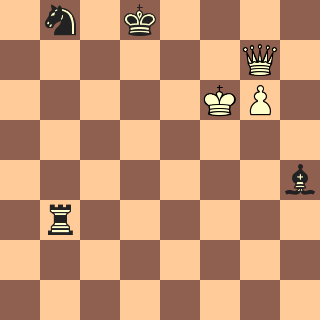
\includegraphics[width=6cm]{fig/mate_in_549}
\caption[Mate in 549]{White to move can mate black in a forced way in an exuberant number of 549 moves. No engine can find the right sequence. This problem is left as an exercise to the reader}
\label{fig:mate549}
\end{figure}

\section{Conclusion}
\label{sec:chessconclusion}

To conclude this chapter, we analyze the characteristics of these approaches. Although chess engines today are much stronger than professional human players (compare the rating of the world champion which is around 2800 with table \ref{tab:engines}), we can never be sure with this approach if the engines are actually making the best decisions. These engines are designed in such a way that they do not play intuitively, but calculate as much variations as possible and base their decision upon that. The choices of variations to look at are based on human expert knowledge, hence the state of the art chess computers have been taught to choose actions in their search tree by human guidelines. \\
These choices have especially their consequences for positional and endgame play, which are far from optimal right now. The static position evaluations have been decided heuristically, which may not have been generalized enough for all chess positions (an example over-coloring this aspect is illustrated in figure \ref{fig:toy}).\\
Due to the tree operations in the search algorithm, there is often overhead by traversing bad lines. A lot of effort has been put in the selection of lines when branching through the tree by introducing heuristics into the move order. If the engines would somehow have better intuition in this idea, the computational effort could decrease.\\
Globally, these methods have already been optimized so much with parallelization and small optimizations, that it may be time to look for different methods to learn more about the beautiful game.

\begin{table}[]
\centering
\caption[Strongest chess engines]{The 12 strongest chess engines, tested by letting them play against each other. These are the playing conditions: Ponder off, General book (up to 12 moves), 3-4-5 piece EGTB
Time control: Equivalent to 40 moves in 40 minutes on Athlon 64 X2 4600+ (2.4 GHz), about 15 minutes on a modern Intel CPU.
Computed on May 27, 2017 with Bayeselo based on 715'938 games \cite{engines}. The strongest FIDE chess rating ever recorded (May 2014) attained by the world champion Magnus Carlsen (at the moment of writing) is included in the ranking for comparison.}
\label{tab:engines}
\begin{tabular}{rrrr}
\toprule
\textbf{Rank} & \textbf{Name} & \textbf{Rating} &\textbf{95\% Confidence} \\
\midrule
1 & Komodo 10.4      & 3392 & $[3372,3412]$ \\
2 & Stockfish 8      & 3390 &  $[3373,3407]$\\
3 & Houdini 5.01     & 3387 & $[3368,3406]$ \\
4 & Deep Shredder 13 & 3288 & $[3268,3308]$ \\
5 & Fire 5           & 3270 & $[3248,3292]$ \\
6 & Fizbo 1.9        & 3249 & $[3225,3273]$ \\
7 & Andscacs 0.89    & 3240 & $[3216,3264]$ \\
8 & Chiron 4         & 3208 & $[3184,3232]$ \\
9 & Gull 3           & 3194 & $[3183,3205]$ \\
10 & Equinox 3.20     & 3186 & $[3174,3198]$ \\
11 & Booot 6.1        & 3178 &  $[3157,3199]$\\
12 & Fritz 15         & 3171 & $[3158,3184]$ \\
&$\cdots$&&\\
58 & Magnus Carlsen & 2882 &\\
\bottomrule
\end{tabular}
\end{table}

\begin{figure}
\centering
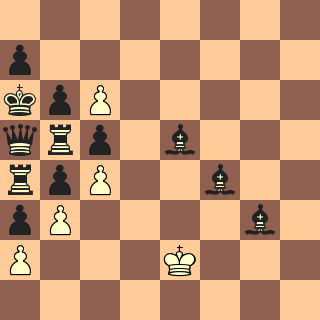
\includegraphics[width=6cm]{fig/diagram_eval}
\caption[Toy example]{A toy example where chess engines fail to indicate the right evaluation. Because the static evaluations are favoring the material value count against the structure in an unbalanced way in this position, the computers indicate black will win almost certainly. In reality, white can actually force this game to be a draw relatively easily \cite{toy}.}
\label{fig:toy}
\end{figure}

\chapter{Deep Learning Background}
\label{ch:background}

In this chapter, we review the mathematical foundations for the methods used in this dissertation. We start of with a walk-through in the world of machine learning (section \ref{sec:ml}) and neural networks (section \ref{sec:nn}), after which we expand on the concept of \acrlong{rl} in section \ref{sec:rl}. These \acrlong{ml} methods are combined into a bigger concept, namely deep \acrlong{rl}.

\section{Machine Learning}
\label{sec:ml}
Machine learning is a family of methods used to perform automatic data analysis gaining insight by finding patterns without having to be explicitly programmed. Due to the incredible growth of data everywhere, machine learning methods are booming in many fields, one of them being \gls{ai}.

Machine learning problems have been classified into three categories, from which hybrids are possible:
\begin{itemize}
\item \textbf{Supervised learning.} The machine has access to labeled data. The labels are true solutions from practice mapped from the given input.
\item \textbf{Unsupervised learning.} In this case, we have no access to labeled data, and the goal is to find some sort of structure in the data points, which we call clusters. 
\item \textbf{Reinforcement learning.} An agent has the task to discover an environment. The environment returns feedback signals (rewards and punishments) to the agent. The goal of the program is to find out how the agent can maximize its rewards. We will dive deeper into this topic in section \ref{sec:rl}.
\end{itemize}

\subsection*{Supervised Learning}
In a supervised learning model, we have access to a dataset $\{(x_1,y_1),\cdots,(x_N,y_N)\}$, with $x_i\in\mathcal{X}$ a feature vector and $y_i\in\mathcal{Y}$ the label corresponding to $x_i$. With the model, we associate a function $f:\mathcal{X}\times\mathcal{W}\mapsto\mathcal{Y}$ with $w \in \mathcal{W}$ denoted as the parameters or weights of the model. This function maps input data to a new label. The goal of a supervised learning algorithm is then to optimize the weights in such a way to minimize a certain loss function $L:\mathcal{Y}\times\mathcal{Y}\mapsto\mathbb{R}_{\leq0}$. In regression problems, where we want to estimate for every new data point $x_i$ a label $\hat{y}_i=f(x_i,w)$, the most common loss function is the \gls{mse}:

\begin{equation}
L=\frac{1}{N}\sum_{i=1}^{N}\left(\hat{y}_i-y_i\right)^2
\label{eq:mse}
\end{equation}

By using a learning algorithm, we try to minimize the loss over the dataset. We then hope that the dataset was a good and diverse representation, such that $f$ generalized well to the real world.\\

Here, we will use combinations of supervised and reinforcement learning to let the computer analyze how chess play can be improved. The data will be collected by an agent in the chess environment, and a supervised learning algorithm can be used on this data.

\section{Neural Network}
\label{sec:nn}

A \acrlong{nn} is a mathematical model typically used in \gls{ml} tasks. The model describes how data points are converted into a class label (in case of classification) or a real value (regression). Then a supervised or unsupervised learning algorithm is applied to a dataset. This learning algorithm tunes the variables in the model in such a way, that it minimizes a certain cost or loss function. In case of supervised (which is what we will use to the highest degree in this thesis), this loss function is a measure of error between the output of the model and a true value from the dataset corresponding with the input. These true values can be seen as the target of the model to reach, as described in section \ref{sec:ml}. \\
Neural networks are a supervised learning model constructed in such a way that they more or less imitate the series of interconnected neurons in the human brain, with the philosophy to let a machine solve recognition and decision tasks in the same fashion as a human being would. We will use this model to estimate the static evaluation function of a chess position.\\

\subsection{Feedforward Neural Network}
\label{subsubsec:ann}

\subsubsection*{Feedforward Propagation}
An \gls{ann} is a \gls{nn} in its most general form, where all nodes in the network can be connected. An \gls{fnn} is an \gls{ann} without the possibility of loops and cycles, as shown schematically in figure \ref{fig:nn}. The computation of the output vector of a given input is called feedforward propagation. Inputs are fed linearly via a series of weights to every node in the first layer. The linear combination of inputs then undergoes a nonlinear transformation called the activation, which at its turn is fed forward into all the layers of the next node and so on and so forth up until the output layer. Nodes in the hidden layer are called hidden units, and are slackly analogous to axons in the human brain. The variables of this model are the weights of the linear combinations, every edge thus corresponds to a tunable parameter. \\


\begin{figure}[htbp]
\begin{center}
\begin{tikzpicture}[scale=1.3]
% 1st column
\node               at (0,0) {};
\node[state] (n0_1) at (0,1) {};
\node		 (n0_2) at (0,2) {$\vdots$};
\node[state] (n0_3) at (0,3) {};
\node		 (n0_4) at (0,4) {$\vdots$};
\node[state] (n0_5) at (0,5) {};
\node               at (0,6) {};
% 2nd column
\node[state] (n2_0) at (2,0) {} 		edge[mainedge] (n0_1) edge[mainedge] (n0_3) edge[mainedge] (n0_5);
\node		 (n2_1) at (2,1) {$\vdots$};
\node[state] (n2_2) at (2,2) {} 		edge[mainedge] (n0_1) edge[mainedge] (n0_3) edge[mainedge] (n0_5);
\node		 (n2_3) at (2,3) {$\vdots$};
\node[state] (n2_4) at (2,4) {} 		edge[mainedge] (n0_1) edge[mainedge] (n0_3) edge[mainedge] (n0_5);
\node               at (2,5) {$\vdots$};
\node[state] (n2_6) at (2,6) {} 		edge[mainedge] (n0_1) edge[mainedge] (n0_3) edge[mainedge] (n0_5);
% 3th column
\node		 (n3_0) at (3,0) {};
\node		 (n3_2) at (3,2) {};
\node		 (n3_4) at (3,4) {};
\node		 (n3_6) at (3,6) {};
% 5th column
\node		 (n5_0) at (5,0) {}	edge[mainedge] (n3_0);
\node		 (n5_2) at (5,2) {}	edge[mainedge] (n3_2);
\node		 (n5_4) at (5,4) {}	edge[mainedge] (n3_4);
\node		 (n5_6) at (5,6) {}	edge[mainedge] (n3_6);
% 6th column
\node[state] (n6_0) at (6,0) {};
\node		 (n6_1) at (6,1) {$\vdots$};
\node[state] (n6_2) at (6,2) {};
\node		 (n6_3) at (6,3) {$\vdots$};
\node[state] (n6_4) at (6,4) {};
\node               at (6,5) {$\vdots$};
\node[state] (n6_6) at (6,6) {};
% 6th column
\node[state] (n8_0) at (8,0) {} edge[mainedge] (n6_0) edge[mainedge] (n6_2) edge[mainedge] (n6_4) edge[mainedge] (n6_6);
\node		 (n8_1) at (8,1) {$\vdots$};
\node[state] (n8_2) at (8,2) {}edge[mainedge] (n6_0) edge[mainedge] (n6_2) edge[mainedge] (n6_4)  edge[mainedge] (n6_6);
\node		 (n8_3) at (8,3) {$\vdots$};
\node[state] (n8_4) at (8,4) {}edge[mainedge] (n6_0) edge[mainedge] (n6_2) edge[mainedge] (n6_4)  edge[mainedge] (n6_6);				
\node               at (8,5) {$\vdots$};
\node[state] (n8_6) at (8,6) {}edge[mainedge] (n6_0) edge[mainedge] (n6_2) edge[mainedge] (n6_4)  edge[mainedge] (n6_6);
% 8th column
\node[state] (n10_1) at (10,1) {} edge[mainedge] (n8_0) edge[mainedge] (n8_2) edge[mainedge] (n8_4) edge[mainedge] (n8_6);
\node		 (n10_3) at (10,3) {$\vdots$};
\node[state] (n10_5) at (10,5) {} edge[mainedge] (n8_0) edge[mainedge] (n8_2) edge[mainedge] (n8_4) edge[mainedge] (n8_6);
% Info
\node[] at (0,-1) {Input Layer};
\node[] at (10,-1) {Output Layer};
\node[] at (5,-1) {Hidden Layers};
\node[] at (-1,3) {$\mathbf{s}$};
\node[] at (11,3) {$\mathbf{v}$};
\node[] at (0.75,6) {$\mathbf{W}^{(0)}$};
\node[] at (7,6.5) {$\mathbf{W}^{(M-1)}$};
\node[] at (9.25,6) {$\mathbf{W}^{(M)}$};
\draw [decorate,decoration={brace,amplitude=5pt},yshift=-15pt] (8,0) -- (2,0);
\draw [decorate,decoration={brace,amplitude=5pt},xshift=-15pt] (0,1) -- (0,5);
\draw [decorate,decoration={brace,amplitude=5pt},xshift=15pt] (10,5) -- (10,1);
\end{tikzpicture}
\end{center}
\caption[General \gls{fnn} architecture]{The general architecture of an \gls{fnn}, also called an \gls{fcn} in literature.}
\label{fig:nn}
\end{figure}

Suppose we have $\mathbf{s}=(s_1,s_2,\dotsc,s_D)$ as input vector, the resulting activation at a node $n \in \{1,\dotsc,N_1\}$ in the first hidden layer is then

\begin{equation}
a^{(1)}_n = \sum_{d=1}^{D} w^{(0)}_{dm} s_d
\end{equation}

where $w^{(0)}_{dm}$ represents the weight between input node $s_d$ and hidden unit $a_n$. We can rewrite all activation equations into matrix form with

\begin{equation}
\mathbf{a}^{(1)}=\mathbf{W}^{(0)^{\mathbf{T}}} \mathbf{s}
\end{equation}

where $\mathbf{W}^{(0)}_{dm}=w^{(0)}_{dm}$. If we call the nonlinear transformation of the activation $\sigma(a)$, the output of every hidden unit yields

\begin{align}
z^{(1)}_{n} &= \sigma (a^{(1)}_{n}) \\
	  &= \sigma \left(\sum_{d=1}^{D} w^{(0)}_{dm} s_d\right)
\end{align}

so we obtain the matrix equation
\begin{equation}
\mathbf{z}^{(1)}=\sigma \left(\mathbf{W}^{(0)^{\mathbf{T}}} \mathbf{s}\right)
\end{equation}

By introducing an additional bias vector at the first layer, allowing translation of every activation function to the desired position, we obtain
\begin{equation}
\mathbf{z}^{(1)}=\sigma \left(\mathbf{W}^{(0)^{\mathbf{T}}} \mathbf{s} + \mathbf{b^{(0)}}\right)
\end{equation}

These calculations are performed in a chain-wise fashion, the outputs of the hidden units in every layer are propagated forward until we arrive at the output layer. Hence, for an arbitrary layer \textit{k}, the the activation equation looks like this (Figure \ref{fig:hu}):
\begin{equation}
\mathbf{z}^{(k)}=\sigma \left(\mathbf{W}^{(k-1)^{\mathbf{T}}} \mathbf{s} + \mathbf{b}^{(k-1)}\right)
\end{equation}

\begin{figure}
\centering
\begin{tikzpicture}
% 1st column
\node        (n0_m2)at (0,-2) {};
\node		 		 at (0,-1) {$\vdots$};
\node		 (n0_0) at (0,0) {};
\node		 		 at (0,1) {$\vdots$};
\node		 (n0_2) at (0,2) {};

% 2nd column
\node[state_small] (n2_0) at (2,0) {$+$} 		edge[mainedge] (n0_m2) edge[mainedge] (n0_0) edge[mainedge] (n0_2);

% 3th column
\node[state_small] (n4_0) at (4,0) {$\sigma$} 		edge[mainedge] (n2_0);

% 4th column
\node		 (n6_0) at (6,0) {} edge[mainedge] (n4_0);

\node at (1.5,-1.5) {$\mathbf{W}^{(k-1)}_m$};
\node at (3,0.5) {$a^{(k)}_m$};
\node at (5,0.5) {$z^{(k)}_m$};

\end{tikzpicture}
\caption[Hidden units]{Hidden unit}
\label{fig:hu}
\end{figure}

The final nonlinear equation describing the feedforward propagation of an \gls{nn} is (supposing we have $M$ hidden layers in total)
\begin{equation}
\mathbf{\hat{v}}=\sigma \left(\mathbf{W}^{(M)^{\mathbf{T}}} \mathbf{s} + \mathbf{b}^{(M)}\right)
\end{equation}

which is the estimate of a value from the gls{NN}, given an input sample.

\subsubsection*{Nonlinearity}
Generally, we want the nonlinear transformation of the activation to be some sort of threshold function (mimicking the biological decision of a neuron to let the information propagate further), but most importantly, it should be a differentiable function. This is because the most commonly used learning algorithm, backpropagation, uses differentiation in its optimization of the \gls{nn}. Due to the recursive nature of the network function and backpropagation, we want the derivative of the activation function to be simple as well. Common choices are the sigmoid, tanh and \gls{relu} function. They are compared in \ref{tab:nonlin}. From these functions, the \gls{relu} seems to provide the best performances in most practical examples \cite{mishkin16}. It should be mentioned that some alternatives like the noisy and leaky \gls{relu} can be used with some success \cite{vinod10,maas14}.

\begin{table}[]
\centering
\begin{tabular}{m{2cm} m{2cm} m{4cm} m{2cm}}
\toprule
\textbf{name} & $\sigma (a)$ & $\sigma'(a)$ & \textbf{chart} \\
\midrule
sigmoid & $\frac{1}{1+e^{-a}}$ & $\sigma(a)(1-\sigma(a))$  &  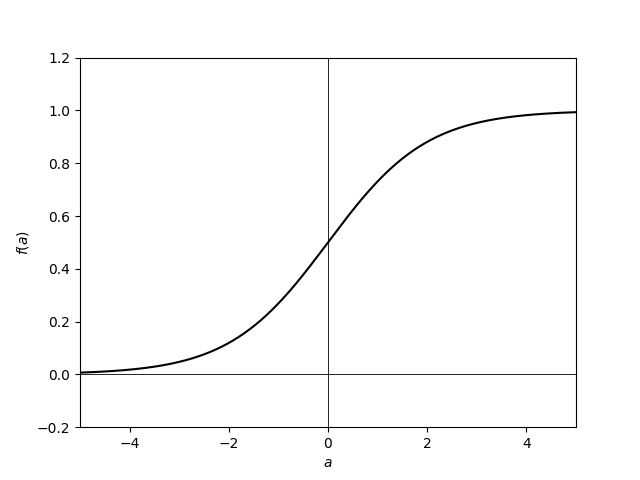
\includegraphics[width=1in]{fig/sigmoid}  \\
tanh & $\tanh(a)$ & $1-\tanh(a)^{2}$&  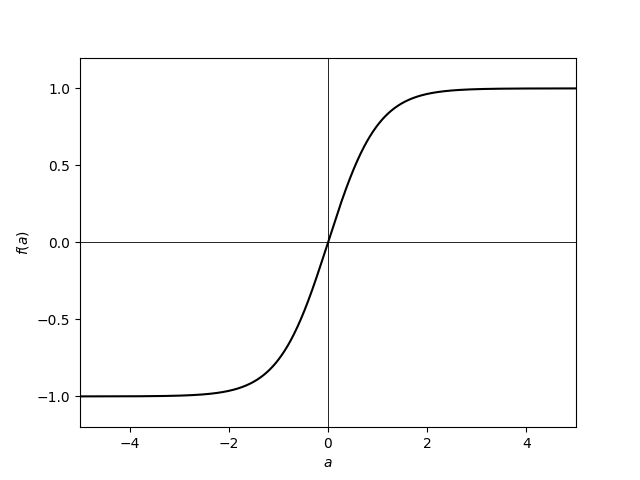
\includegraphics[width=1in]{fig/tanh}        \\
ReLU & $\max(a,0) $ & 
$
  \begin{cases} 
   1 & \text{if } a > 0 \\
   0       & \text{if } a \leq 0
  \end{cases}
$      &  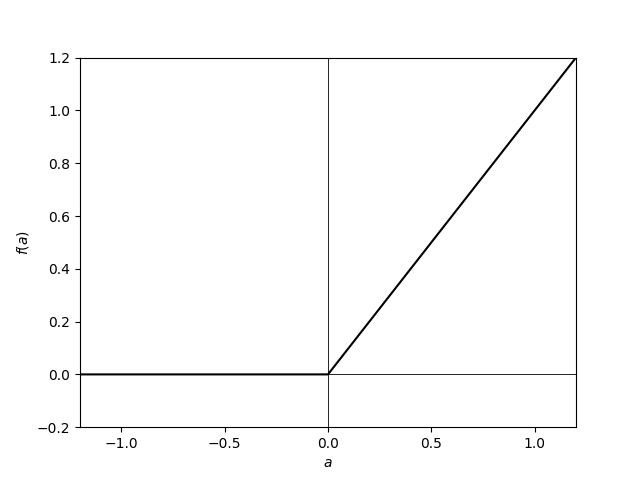
\includegraphics[width=1in]{fig/relu}          \\
\bottomrule
\end{tabular}
\caption[Comparison between activation functions]{Comparison between activation functions}
\label{tab:nonlin}
\end{table}

\subsubsection*{Learning Algorithm}
The goal of the learning algorithm is to tune all model parameters (the weights and bias) such that a global loss function on the training data is minimized. Supposing we have $N$ data samples available, we write 
\begin{equation}
L(w)=\frac{1}{N} \sum_{i=1}^{N} L_i(w)
\end{equation}

so we want to minimize the sum of all errors on all individual samples. The choice of $L_i(w)$ depends on the chosen problem.\\
To find a local optimum, most researchers use gradient descent, a first-order iterative optimization algorithm. It may not find the global optimum, but it is computationally efficient, because of the ease at finding the first partial derivatives of all weights with backpropagation. By updating the weights in the direction of the steepest descent (the gradient of the loss function with respect to all parameters) at each iteration, we gradually reduce the global loss.
\begin{align}
w &\leftarrow w-\alpha\nabla L(w) \\
&=w-\alpha\sum_{i=1}^{N}\frac{\nabla_w L_i(w)}{N}
\end{align}

We observe the introduction of a new training parameter, the step size in the steepest direct also called the learning rate $\alpha$. It should be chosen wisely. The higher the learning rate, the faster the model will learn a local optimum, but if it is too big it might oscillate around the ravine. In contrast, the learning algorithm will be slower but more accurate for a smaller step size. \\
As our problem to approximate the static evaluation function of a chess position is a regression problem, we will use the \gls{mse} from section \ref{sec:ml}. By calculating the derivative we find the update rule for the weights to be

\begin{align}
w&\leftarrow w-\alpha\sum_{i=1}^{N}\frac{\nabla_w L_i(w)}{N} \\
& =w-\frac{\alpha}{N}\sum_{i=1}^{N}\nabla_w\left(\hat{y}_i(w)-y_i\right)^2 \\
& =w-\frac{\alpha}{N}\sum_{i=1}^{N}\left(\hat{y}_i(w)-y_i\right)\nabla_w\hat{y}_i(w)
\end{align}

The issue with using gradient descent as described above, is that it can be computationally expensive to perform a single step, as we have to run through the whole training set. By updating the model parameters in an online manner, i.e. update the model along every sample of the dataset, we achieve a faster convergence rate. This has to happen stochastically (we need to shuffle the dataset at every iteration). With the theories of convex minimization and stochastic approximation, it has been proven that almost surely the objective function will converge to a local minimum \cite{saad98}. The name of this online learning algorithm is \gls{sgd}\\
One remaining problem is that computing every update independently is slower that computing them in batch with vectorization libraries (eg. LAPACK). The solution to this problem is straightforward, we can make a compromise between gradient descent and \gls{sgd} by doing the weight updates in minibatches. A high-level pseudo code description is laid out in Algorithm \ref{al:gd}\\
 
\begin{algorithm}
  \caption{Minibatch stochastic gradient descent}
  \label{al:gd}
  \begin{algorithmic}
  	\REQUIRE $S$,$V$,$n$
  	\COMMENT{$n$ is size minibatch, $1\rightarrow$SGD, $N\rightarrow$GD}
	\STATE Initialize $w$ (randomly),$\alpha$
	\REPEAT
		\STATE shuffle samples \\
		\FOR{all minibatches}
			\STATE $w \gets w-\alpha\sum_{i=1}^{n}\frac{\nabla L_i(w)}{n}$
		\ENDFOR
	\UNTIL local minimum is achieved
  \end{algorithmic}
\end{algorithm}

\subsubsection*{Further optimizations}

We initialize the weights $w$ with random values. It is intuitive to understand that at the start of learning, we are allowed to make bigger steps into the right direction. Then, we could gradually decrease the value of the learning. In other words, it makes sense to use adaptive learning rates. Two notable and widely accepted adapted gradient mechanisms are \textit{AdaGrad} (which bases its learning rate updates on weight changes so far) and \textit{RMSProp} (less aggressive form of \textit{AdaGrad}) \cite{duchi11,sutskever12}.

To reduce the oscillation of the random fluctuations of online learning, researchers came up with the momentum method, which (just like a real object) follows the steepest descent until it has enough velocity to deviate from it into the previous direction. The most famous momentum gradient descent learning algorithm is the \textit{Nesterov} momentum. There are a lot more variations on standard minibatch \gls{sgd}, for which I encourage the reader to read \textit{Deep Learning} \cite{Goodfellow-et-al-2016}.

\subsubsection*{Backpropagation}
As described in the previous subsection, we need to calculate the gradient of the loss function with respect to the weights of all connections. The backpropagation algorithm is an efficient recursive algorithm achieving this goal. As the name suggests, we start by calculating the derivatives in the last layer, and let the information we get from calculating these derivatives propagate backwards to compute the weight derivatives of previous layers all the way back to the input layer. This is done with the chain rule of differentiation. More specific details and a proof can be found in \textit{Deep Learning}.\\

\subsection{Convolutional Neural Network}
\label{subsubsec:cnn}
To further simulate the functioning of the brain and apply it to machine learning tasks, researchers created \acrlong{cnn}s, a feedforward \gls{ann} where weights are shared between spatially correlated neurons, to give the network understanding of translation invariance. The connectivity pattern of neurons is inspired by the visual cortex. They have been applied successfully especially in the field of computer vision, but also in other domains. The main resource for this section is \textit{Deep Learning} \cite{Goodfellow-et-al-2016}.\\

Convolutional layers are the core building blocks of \gls{cnn}s, after which an \gls{fcn} computes the output. These layers are stacks of feature maps. The deeper we go into the architecture, the larger the receptive field of every hidden unit, i.e. the number of input parameters that had an influence on the hidden node. The connections between neurons are filters. The idea is thus to learn the optimal filters we have to apply onto the receptive fields in order to achieve the best features possible in the next layer. Feedforward computations are accomplished with the convolution operation, hence the name.\\
We will later see in the next chapter how this architecture may be beneficial for the performance of board games like \textit{go}, and maybe chess.

\subsubsection*{Convolution}
The convolution \footnote{The presented convolution is actually a cross correlation in mathematics terminology} operation is the application of weighted averaging of correlated measurements to account input noise into the output. We do this averaging for every input variable around its center. Suppose we have a 1-D tensor of discrete measurements, we write this down mathematically as 
\begin{align}
y(i) &= (w \ast x)(i)\\
&= \sum_{n} w(n) x(i+n)
\end{align}

For 2-D data (as images for instance) this convolution is 
\begin{align}
Y(i,j) &= (W \ast X)(i,j)\\
&= \sum_{m,n} W(m,n) X(i+m,j+n)
\end{align}

which are actually 2 1-D convolutions at the same time. The weight matrix is also called the kernel in machine learning terminology, while the filters are called kernels.\\

Why can using the convolution operation be so beneficial for machine learning tasks? It provides three important characteristics: sparse interactions, parameter sharing and equivariant representations \cite{goodf16}.\\
The sparse interactions are attained by making the kernel smaller than the input, resulting in having to store less parameters. \\
Secondly, tied weights are used, which means that all windows of feature maps are transformed by the same kernels into the next layer. This as well reduces the size of the parameter space, but has also the consequence that instead of learning a separate set of parameters for every location of the input like in a simple \gls{fnn}, the parameters will be shared location independently. Hence, the model becomes translation invariant. The parameter sharing and sparse interactions are visualized in \ref{fig:ps}.\\
The equivariance relationship ($f$ and $g$ are equivariant functions if and only if $f(g(x))\equiv(g(f(x)))$) is therefore attained for translation, but it can be achieved for other relations (eg. scale, rotation) as well by using different mechanisms.
\begin{figure}
\centering
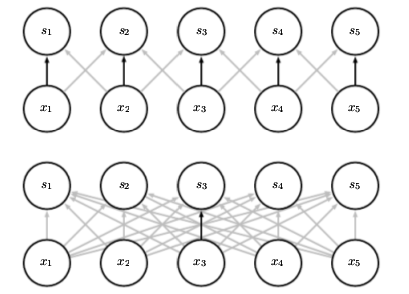
\includegraphics[scale=0.7]{fig/param_sharing}
\caption[Connections \gls{fnn} and \gls{cnn}]{In an FCN, all units between layers are connected to each other, but in a CNN the nodes are only connected by the nodes from its receptive field in the previous layer. This makes the number of connections considerably smaller. The weights are also equal for every connection set between input nodes.}
\label{fig:ps}
\end{figure}

\subsubsection*{Convolutional Layer Architecture}
Convolutional layers typically consist out of 3 main stages as shown in figure \ref{fig:cnn}. The input is fed into the convolutional stage, which executes the convolution operations. This is followed by a nonlinear transformation just as in section \ref{sec:nn}. The convolutional layer can be finalized by an optional pooling stage if the model is used for computer vision purposes. The output of the last stage is then the input is then fed into the next convolutional layer, making \gls{cnn}s a feedforward architecture.\\
Pooling is a method to introduce extra invariances by downsampling the information. Additional information can be found in the references, but this method is not from crucial importance to this master dissertation \cite{boureau11}.\\

\begin{figure}
\centering
\begin{tikzpicture}
% 1st column
\node[staterect] (n0_0) at (0,0) {Input};
\node[staterect] (n0_2) at (0,-2) {Convolutional Stage} edge[mainedge] (n0_0);
\node[staterect] (n0_4) at (0,-4) {Nonlinear Stage} edge[mainedge] (n0_2);
\node[staterect] (n0_6) at (0,-6) {Pooling Stage} edge[mainedge] (n0_4);
\node[staterect] (n0_8) at (0,-8) {Output} edge[mainedge] (n0_6);
\draw (-3,-1) rectangle (3,-7);
\node[scale=0.75] at (1.5,-7.25) {Convolutional Layer};

\end{tikzpicture}
\caption{Convolutional layer flow diagram}
\label{fig:cnn}
\end{figure}

\subsection{Deep learning}
\label{subsubsec:dl}
Deep learning algorithms are (as the name suggests) neural networks using an architecture with many hidden layers. The conditions for an architecture to be 'deep' are that \cite{deng14}:
\begin{itemize}
\item it is a composition of successive layers, using the output of previous layer as input
\item it is based on hierarchical learning of feature representations of the data. The features learned in deeper layers are more complex and are derived from the low level features learned in earlier stages of the network.
\item learn multiple representations on different abstractions
\end{itemize}

\section{(Deep) Reinforcement Learning}
\label{sec:rl}

Just like neural networks are inspired by the functioning of the brain, \gls{rl} is a field in machine learning inspired by behaviorist psychology. The principal idea of solving problems in \gls{rl} is to find from any given situation in an environment the optimal sequence of actions such that an agent in the environment maximizes its reward. The bigger the rewards, the closer the agent is to achieving its final goal. The agent has to find this sequence by exploring the environment, where actions in given states lead to certain rewards. To better understand the environment and increase future rewards, the agent has to balance between exploiting current knowledge and exploring new areas of the environment where he knows less about, this is the exploration-exploitation dilemma. \\

\begin{figure}
\centering
\begin{tikzpicture}
\node[staterect] (n0_0) at (0,0) {Agent} edge[mainedge, bend left] (n0_4);
\node[staterect] (n0_4) at (0,-4) {Environment: $s_t$} edge[mainedge, bend left] (n0_0);
\node at (-1,-2) {$a_t$};
\node at (1.1,-2) {$r_{t+1}$};
\node at (1.1,-2.5) {$s_{t+1}$};
\end{tikzpicture}
\caption[\gls{rl} paradigm]{The general framework for \gls{rl}, an agent is performing an action $a_t$ in state $s_t$. By doing this action, it will receive its new state $s_{t+1}$ with the reward $r_{t+1}$ corresponding to the action at the next time step.}
\label{fig:rl}
\end{figure}

We start of this section with an explanation about Markov decision processes, the mathematical framework used for studying \gls{rl}. We will find out that for an agent to interpret its environment better, it should sense which states are best to reside in. Background on these problems are provided in section \ref{subsec:vp}. Similarly, we want to know which actions the agent should take to understand its environment to the best of his powers, this is examined in \ref{subsec:control}. This section is concluded with algorithms using value prediction as well as control in section \ref{subsec:iter}.

\subsection{Markov Decision Process}

Notations are inspired on the survey \textit{Algorithms for Reinforcement Learning} \cite{szepe10}.
\label{subsec:mdp}
\begin{definition}
An \gls{mdp} is a 5-tuple $\mathcal{M}=(\mathcal{S,A,P},R,\gamma)$ with
\begin{itemize}
\item $\mathcal{S}$: state space
\item $\mathcal{A}$: action space
\item $\mathcal{P}: \mathcal{S} \times \mathcal{A} \times \mathcal{S} \mapsto \mathbb{R} $: state transition probability kernel
\item $R: \mathcal{S} \times \mathcal{A} \mapsto \mathbb{R} $: the expected immediate reward function
\item $\gamma \in \mathbb{R} \cap (0,1) $: discount factor
\end{itemize}
\end{definition}

With \gls{mdp}s we can define sequential decision making problems in \gls{rl} as follows. Suppose $t \in \mathbb{N}$ denotes an instant of time, and we interact according \gls{mdp} $\mathcal{M}$. When an agent chooses action $a_t \in \mathcal{A}$ in state $s_t \in \mathcal{S}$, it gets fed back a reward $r_{t+1}$ and arrives in a new state $s_{t+1}$ with a probability $P(s_{t+1}|s_t,a_t)$. The expected reward at time step $t$ was $R(s_t,a_t)$, but from now on we assume this reward to be deterministic given $a_t$ and $s_t$ to simplify the framework. \\
From this point on, the same decision process goes on and on until the agent arrives at a terminal state $s_T$. A full sequence $\{s_1,s_2,\dotso,s_T\}$ is called an episode. The goal of the agent is to maximize its return over the course of an episode. The return starting from $t$ is defined as the exponentially discounted sum of the rewards obtained:
\begin{equation}
\mathcal{R}=\sum_{t=0}^{\infty}\gamma^t r_{t+1}
\end{equation}
In this manner, MDPs can balance between being discounted ($\gamma<1$) and undiscounted ($\gamma=1$).
The agent bases its future behavior on the history up until we arrived at $s_t$ is defined by the sequence of tuples $(s_0,a_0,r_1),(s_1,a_1,r_2), \dotso , (s_{t-1},a_{t-1},r_t)$. \\
From this point on, we will assume the \gls{mdp} to be deterministic, i.e. only one state transition $s_{t+1}$ is possible given $(s_t,a_t)$. To formally describe this, define the successor function $\Sigma: \mathcal{S} \times  \mathcal{A} \mapsto \mathcal{S}$. The state transition probability kernel simplifies to
\begin{equation}
P(s_{t+1}|s_t,a_t) = \left\{
  \begin{array}{ll}
    1 & \Sigma(s_t,a)=s_{t+1}\\
    0 & else
  \end{array}
\right.
\label{eq:det}
\end{equation} 

In the next chapter, we will see how chess can easily fit into this framework of \gls{mdp}s as a tool to learn to play chess.

\subsubsection*{Value Function}
Before we continue, we define the concept of a policy.
\begin{definition}
A policy is a probability function $\pi:\mathcal{S} \times \mathcal{A} \mapsto \mathbb{\mathbb{R}}$. An agent is following a policy $\pi$ if it draws its next action $a \in \mathcal{A}$ in state $s \in \mathcal{S}$  randomly with probability $\pi(a|s)$
\end{definition}
To find the optimal behavior in an \gls{mdp}, value functions are used. Value functions denote how good it is for an agent to be in certain states. For chess boards, this is equivalent to the static evaluation function.
\begin{definition}
The value function $V^{\pi}:\mathcal{S}\mapsto\mathbb{R}$ with underlying policy $\pi$ is defined by
\begin{equation}
V^{\pi}(s) = \mathbb{E}\left[\mathcal{R}|s\right] = \mathbb{E}\left[\sum_{t=0}^{\infty}\gamma^t r_{t+1}|s\right]
\label{eq:v}
\end{equation}
with the understanding that all triplets $(s_t,a_t,r_{t+1})$ came up by following $\pi$.
\end{definition}

In contrast to value functions, action value functions stand for the profit achieved by performing an action in a certain state.

\begin{definition}
The action value function $Q^{\pi}:\mathcal{S} \times \mathcal{A} \mapsto\mathbb{R}$ with underlying policy $\pi$ is defined by
\begin{equation}
Q^{\pi}(s,a) = \mathbb{E}\left[\mathcal{R}|s,a\right] = \mathbb{E}\left[\sum_{t=0}^{\infty}\gamma^t r_{t+1}|s,a\right]
\end{equation}
with the understanding that all triplets $(s_t,a_t,r_{t+1})$ came up by following $\pi$.
\end{definition}

An optimal policy can be derived easily supposing we have found the optimal value for every state in the state space, which is the highest achievable return starting from a state. The optimal value function $V^*:\mathcal{S}\mapsto\mathbb{R}$ attains this most favorable mapping. We define the optimal action value function $Q^{*}:\mathcal{S} \times \mathcal{A}$ analogously. The policy performing greedy actions only with respect to $Q^*$ is an optimal policy. As we can relate $V^*$ and $Q^*$ to each other by the coming equations:

\begin{align}
V^*(s) &= \max_{a \in A} Q^*(s,a) \\ 
Q^*(s,a) &= R(s,a) + \gamma V^*(\Sigma(s,a))
\end{align}

we can also act optimally according to $V^*$ by acting greedily with respect to the next state's value function.\\

The remaining question is now on how to find these optimal functions. A tool used for this are the recursive Bellman equations \cite{bert07}.
\begin{theorem}
The optimal value function satisfies
\begin{equation}
V^*(s) = \max_{a \in A} \left\{R(s,a) + \gamma V^*(\Sigma(s,a))\right\}
\end{equation}
The optimal action value function satisfies
\begin{equation}
Q^*(s,a) = R(s,a) + \gamma \max_{a'\in \mathcal{A}} Q^*(\Sigma(s,a),a')
\end{equation}
\end{theorem}

\subsection{Value Prediction}
\label{subsec:vp}

\subsubsection*{Monte Carlo method}
Let us consider the problem of the estimation of the value function. The closer we can approach the optimal value function with our estimate, the better our policy will be. We defined the value function earlier as the expected return starting from a certain state \ref{eq:v}. This definition gives us the insight that a possible algorithm to create approximations might be a Monte Carlo algorithm, averaging out all returns.\\
Suppose we have got an \gls{mdp} $\mathcal{M}=(\mathcal{S,A,P},R,\gamma)$ that generated $N$ episodes following a certain policy, with each episode having an index $n$ and history \[H_n=\left\{(s_0,a_0,r_1),(s_1,a_1,r_2), \dotso , (s_{T_{n}-1},a_{T_{n}-1},r_{T_{n}})\right\}\] Store the observed returns for every state in time in every episode
\begin{equation}
\mathcal{R}_n(t)=\sum_{t'=t}^{T_{n}-1}\gamma^{t'-t} r_{t'+1}
\end{equation}
We can now sensibly update the value function after the termination of an episode with a gradient descent kind of optimization step with the following update function
\begin{equation}
\hat{V}(s_t) \leftarrow \hat{V}(s_t)+\alpha\left(\mathcal{R}_n(t)-\hat{V}(s_t)\right)
\end{equation}
where $\alpha$ is the learning rate and $\mathcal{R}_n(t)-\hat{V}(s_t)$ is the gradient of the \gls{mse} between the actual observed return and the estimated return. We can find a nice recursive relationship between observed returns in an episode:
\begin{align*}
\mathcal{R}_n(T-1) &= r_{T} \\
\mathcal{R}_n(t)&= r_{t+1}+\gamma \mathcal{R}_n(t+1)
\end{align*}
This recursive relation is used in Algorithm \ref{al:evmc}, where the history of an episode is interpreted to update the value function. The presented algorithm is called the \gls{evmc} algorithm. At the moment, we are assuming tabular methods, where the value function is stored for each distinct state independently in an array.

\begin{algorithm}
\begin{algorithmic}
\REQUIRE $H=\left\{(s_0,a_0,r_1),(s_1,a_1,r_2), \dotso , (s_{T_{n}-1},a_{T-1},r_{T})\right\},V(s)$
\STATE $\mathcal{R}_n \leftarrow 0$
\FOR{$t \leftarrow T-1$ \textbf{downto} $ 0$}
\STATE $\mathcal{R}_n \leftarrow r_{t+1}+\gamma \mathcal{R}_n$
\STATE $V(s_t) \leftarrow V(s_t)+\alpha\left(\mathcal{R}_n-V(s_t)\right)$
\COMMENT{Gradient Descent update step}
\ENDFOR 
\end{algorithmic}
\caption{Episodical EMVC}
\label{al:evmc}
\end{algorithm}

In practice, \gls{evmc} stabilizes for the tabular method (which is only feasible for a limited amount of states) almost surely to the optimum. The issue is the variance between the calculated returns over episodes, which can be very high because we take every visited state into account (this is a general problem of \gls{mc} simulations in general \cite{robert05}), resulting in poor estimates at first and a long training time. \\

\subsubsection*{TD(0)}
To address the issues of \gls{evmc}, we will limit the influence of states further away in the episode with temporal difference learning, the most drastic one being TD(0), where we only use the value of the next state in our estimate. As in \gls{evmc}, we will use an online gradient descent algorithm. The update function is now (under the same \gls{mdp} conditions as in the MC method described earlier)
\begin{equation}
\hat{V}(s_t) \leftarrow \hat{V}(s_t)+\alpha\left(r_{t+1}+\gamma\hat{V}(s_{t+1}) -\hat{V}(s)\right)
\end{equation}
So basically, we have slightly modified the target for a state to a linear approximation of the true return in the episode. The TD-error is $r_{t+1}+\gamma\hat{V}(s_{t+1}) -\hat{V}(s)$. States further away than the next state do not influence the target anymore. These were exactly the states entailing the largest amount noise in \gls{mc} measurements. Another advantage over \gls{evmc} is its suitability for incremental learning, meaning we can update our value function after every action, as in algorithm \ref{al:td0}.

\begin{algorithm}
\begin{algorithmic}
\REQUIRE $s_t,r,s_{t+1},V$
\STATE $V(s_t) \leftarrow V(s_t)+\alpha\left(r_{t+1}+\gamma V(s_{t+1}) -V(s_t)\right)$
\COMMENT{gradient descent update step}
\end{algorithmic}
\caption{TD(0)}
\label{al:td0}
\end{algorithm}

Just like \gls{evmc}, TD(0) converges almost surely to $V^*$. One may wonder which algorithm works best and in which cases, as they both have their own merits. An example where TD(0) is slower than \gls{evmc} is a long chain of states where the agent only gets a positive reward at the final action, because the TD-error has to propagate back to the first states. So the longer the chain, the longer it will take until the initial states have learned which paths to follow.

\subsubsection*{TD($\lambda$)}
The attentive reader may have wondered why temporal difference learning is called TD(0). The reason behind the zero in the name is because it is actually a special case of TD($\lambda$), an algorithm unifying \gls{evmc} and TD(0). First of all, let us define the $n$-step return, which is a prediction of the actual return taking $n$ states ahead into account.
\begin{equation}
\label{eq:nstep}
G_n(t)=\left(\sum_{i=0}^{n-1}\gamma^i r_{t+i}\right)+\gamma^n V(s_t+n)
\end{equation}
We notice $G_1(t)$ to be the target return in TD(0) and $G_{T-t}(t)$ the real return value given $T$, the length of the episode. We construct the $\lambda$-return with all n-step returns with exponential decay as mixing weights.
\begin{equation}
\label{eq:tdlambda_inf}
G_{\lambda}(t)=(1-\lambda) \sum_{n=1}^{\infty} \lambda^{n-1}G_n(t)
\end{equation}
where it can easily be checked that $(1-\lambda)$ is a normalization factor. $\lambda$ is the trace decay parameter, and controls to what extent the algorithm resembles on TD(0) or a Monte Carlo algorithm. $\lambda=0$ gives TD(0). The finite version of equation \ref{eq:tdlambda_inf} is
\begin{equation}
\label{eq:tdlambda_fin}
G_{\lambda}(t)=(1-\lambda) \sum_{n=1}^{T-t} \lambda^{n-1}G_n(t) + \lambda^{T-t} G_t
\end{equation}
where we define $G_t$ to be all the subsequent $n$-step returns after the terminal state. \\
An incremental algorithm can be designed by using accumulating eligibility traces, which can be seen as some sort of history of past states. The TD-error propagates back to all past states when the incremental update occurs. Suppose $z$ is the eligibility trace, appropriate incremental updates are then \cite{sutton98}
\begin{align}
z(s_t) &\leftarrow 1+\gamma \lambda z(s_t) \\
V(s_t) &\leftarrow V(s_t)+\alpha\left(r_{t+1}+\gamma V(s_{t+1}) -V(s_t)\right)z(s_t)
\end{align}
Algorithm \ref{al:tdy_tab} gives pseudocode for a tabular TD($\lambda$) algorithm 

\begin{algorithm}
\begin{algorithmic}
\REQUIRE{$s_t, r_{t+1}, s_{t+1}, V, z$}
\FOR{$s \in \mathcal{S}$}
%\COMMENT{it is only necessary to look at the states in history episode}
\STATE{$z(s) \leftarrow \gamma \lambda z(s) + \mathbbm{1}_{\{s=s_t\}}$}
\STATE{$V(s) \leftarrow V(s)+\alpha\left(r_{t+1}+\gamma V(s_{t+1}) -V(s_t)\right)z(s_t)$ }
\ENDFOR
\end{algorithmic}
\caption{Tabular TD($\lambda$)}
\label{al:tdy_tab}
\end{algorithm}

In summary, TD($\lambda$) tries to assemble the advantages of both TD-learning and Monte Carlo methods. Just as these algorithms, it converges to $V^*$. Finding the right value of $\lambda$ for quicker convergence is often a process of trial and error, and it has even been proved that changing $\lambda$ during training does not impact convergence under the right circumstances (eg. eligibility trace update function) \cite{bert96}.

\subsubsection*{Function approximation}
The methods considered so far consider a tabular value function, but many problems like chess have such a large state space that saving all their values is infeasible. We choose to describe all states with feature vectors. A state $s \in \mathcal{S}$ is transformed to its feature vector of dimension $D$ by a feature extraction method $\phi: \mathcal{S} \mapsto \mathbb{(R)}^D$. The value function can then be constructed around a mathematical model operating on these feature vectors $\phi(s)$. This model introduces a new set of parameters, the weights $w$ of the model. \\
Some examples of function approximation methods are
\begin{itemize}
\item linear: $V_w(s)=w^T \phi(s)$
\item neural networks (see Section \ref{sec:nn})
\item other mathematical models for machine learning 
\end{itemize}

Deep \gls{rl} is the class of \gls{rl} algorithms using deep neural networks as function approximation method. From now on it is assumed neural networks are used for this task. The tabular methods we have discussed so far now needs to be generalized to algorithms with function approximation. As Monte Carlo algorithms and TD(0) can be seen as special cases of TD($\lambda$), we will limit our examination to TD($\lambda$). An example of a non incremental episodic learning algorithm works as follows:
\begin{enumerate}
\item run episode and get history $\mathcal{H}_n$
\item calculate the $\lambda$-returns for all states in $\mathcal{H}_n$
\item use the $\lambda$-returns as target values for supervised learning on a neural network.
\item update weights of neural network with gradient descent 
\end{enumerate} 
As we want to learn a continuous value function, this is a regression problem. A classical loss function to optimize in regression problems is the Mean Squared Error (MSE): $L_w(\hat{V},V)=(\hat{V}-V)^2/2$. \\
When using non-linear value function approximators, convergence is no longer guaranteed \cite{baird95}.However, the algorithm generally still finds good results in practice  under the right choice of hyper-parameters.

\subsection{Control}
\label{subsec:control}
We primarily focus on learning problems where the agent can influence its observations, which is interactive learning. The agent is making decisions changing the state of the environment and improving its policy. There are two ways for the agent to improve its policy. It can use active learning, where it will control the samples such that it maximizes finding a good policy or it can use online learning, where the online performance is optimized.

\subsubsection{Closed-loop Online Learning}
\label{subsec:clil}
It is from crucial importance in online learning to occasionally choose  actions that at the time might look suboptimal, to augment the future payoff. This question is then how frequent the agent must balance its choice to explore or exploit the current environment. This means that the methods described in this section can be used independently from which value functions are used. \\

\textbf{$\epsilon$-greedy policy}
This is a very simple strategy to balance exploitation and exploration, choose a fixed parameter $\epsilon \in \mathbb{R} \cap [0,1]$ and at every state choose a random action with probability $\epsilon$. Although this method is really simple, it can be competitive with more sophisticated algorithms if we some time decay is employed and tuned. Time decay is beneficial as normally the policy should improve, hence we should exploit more as time goes on. \\

\textbf{Boltzmann exploration strategy}
With $\epsilon$-greedy, actions are drawn uniformly with a probability $\epsilon$. We may want to draw seemingly worse actions with a lower probability. To attain this property, we can use the distribution
\begin{equation}
\pi(a|s)=\frac{e^{\beta J(s,a)}}{\sum_{a' \in \mathcal{A}_s} e^{\beta J(s,a)}}
\end{equation}
$\beta$ controls how greedy the action will be, while $J: \mathcal{S} \times \mathcal{A} \mapsto \mathbb{R}$ is a function indicating how good the action is, like $V(\Sigma(s))$ or $Q(s,a)$. 

\subsubsection{Q-learning}
By trying to learn $Q^*$ immediately, a greedy policy may be close to optimal.

With tabular Q-learning, an estimate for every $(s,a)$-tuple is stored and updated incrementally. Just as in TD-learning, this update happens in a gradient descent manner, by moving the Q-value in the direction of the last error between the target and previous estimate. Upon the observation of $(s_t,a_t,r_{t+1},s_{t+1})$, the Q-value changes to
\begin{equation}
Q(s_t,a_t) \leftarrow Q(s_t,a_t)+\alpha \left(r_{t+1}+\gamma \max_{a' \in \mathcal{A}} \left\{ Q(s_{t+1},a')\right\}-Q(s_t,a_t)\right)
\end{equation}
Analogous to TD-learning, the target value of our estimate is $r_{t+1}+\gamma \max_{a' \in \mathcal{A}} \left\{ Q(s_{t+1},a')\right\}$. \\
Q-learning is very attractive due to its simplicity, and its convergence to $Q^*$. The policy followed by the agent could be $\epsilon$-greedy or \textit{Boltzmann} exploration. \\
Incremental Deep Q-learning algorithms can then be generated with the extension to function approximation for $Q_w$:
\begin{equation}
w \leftarrow w+\alpha \left(r_{t+1}+\gamma \max_{a' \in \mathcal{A}} \left\{ Q_w(s_{t+1},a')\right\}-Q_w(s_t,a_t)\right) \nabla_w Q_w(s_t,a_t)
\end{equation}
This update rule is used plenty of times in practice. However, its convergence properties are doubtful to say at least, especially when non linear approximation methods like deep learning are used. \\

Analogous to our deep TD($\lambda$) algorithm, we can use episodic experience to learn the optimal weights of our network with regression. Good empirical results have been obtained by adding new samples to the data used for the previous iteration \cite{ried05}.

\subsection{Value and Policy Iteration}
\label{subsec:iter}
The presented Q-learning and TD-learning algorithms are value iteration algorithms, by exploring the environment the value function changes up until the point it has converged. There are two weaknesses to applying value iteration only:
\begin{itemize}
\item may take a long time to converge
\item we actually try to find the optimal policy, the value function is just a tool to do so
\end{itemize}
To incorporate the updates of policies, we can iterate over value iteration and policy iteration.
\begin{enumerate}
\item pick a random policy $\pi$
\item update $V^{\pi}$ under the policy
\item improve $\pi$
\item go back to step 2 if satisfied
\end{enumerate}
We actually already discussed a value and policy iteration algorithm, namely the use of the \textit{Boltzmann} distribution to choose the next action. In that example, we updated the policy in an incremental fashion, as there is an immediate relationship between the policy and the value function.


\chapter{Deep Reinforcement Learning in Chess (and other games)}
\label{ch:drlgames}
In this chapter, we will explore how we can use deep \gls{rl} and mechanisms discussed in previous chapters to let a machine play games, and chess especially as it is the main focus of this dissertation. As we will have to feed chess positions into the neural networks, we will have to transform them into a vector representation. One should not forget that the starting point of the machine should be only knowledge about the game, and no expert knowledge. How this is done and how we can do it in chess is discussed in section \ref{sec:fs}. We need a function transforming this vector data into an evaluation, this is considered in \ref{sec:sef}. The application of TD($\lambda$) and more sophisticated versions of TD-learning to games is further examined in section \ref{sec:td}. A method that has shown recent success is presented in section \ref{sec:mcts} and we conclude this chapter by also considering how we could introduce policy iterations into chess in section \ref{sec:polnet}.

\section{Feature Space}
\label{sec:fs}
Because the state space of most games is excessively big, tabular methods have no chance of being successful. This fact justifies using function approximation on a vectorized representation of game states. The feature vector is then fed into a machine learning framework of choice, often (deep) neural networks and \gls{cnn}s.\\

The goal of our feature vector should be general and low level enough, to avoid being biased by the features. Let us examine the chess representations used by other machine learning engines for inspiration.\\
In section \ref{sec:evaluation} we already described how most engines represent the chess position with handcrafted expert features among features that only contain knowledge strictly characteristic to the model of the game. Also \textit{Meep}, a \gls{rl} based chess program, maintains
\begin{itemize}
\item material
\item piece square tables
\item pawn structure
\item mobility
\item king safety
\end{itemize}
information in a mostly binary fashion, which makes it a sparse representation \cite{veness09}. To arrive to a unbiased and general representation of the chess board, we will combine ideas from computer vision and another board game, \textit{go}. \\

Nowadays, most object recognition and category learning tasks in computer vision are performed with the help of deep neural networks, especially CNNs. These networks take raw image data over several channels (often a separate channel for each color channel) as input, and the actual knowledge is learned over the course of several layers \cite{kriz10}. This is in contrast of using a different model with features obtained by image analysis like \textit{histogram of gradients} and a \textit{bag of words} representation extracted with help of clustering over a large dataset \cite{lowe04}. This idea propagated further into the \gls{rl} field with \textit{Atari} games, where deep Q-learning is applied on raw image data as state representations \cite{silv13}. The climax was reached when researchers implemented \textit{AlphaGo}. This engine mastered \textit{go} through self play and feeding board positions as a stack of binary image data into a CNN to learn the evaluation function with supervised learning \cite{alphago16}.\\

We can try to do the same in chess as in go, by stacking up feature planes describing the position and mobility of the pieces in a binary fashion. We will call these maps the piece maps and mobility maps. The idea used is the same as the concept of bitboards, a data structure commonly used in chess engines to describe a board state. A bitboard is defined as an array with the dimension of a chessboard ($8\times8$), where each element describes the state of the square with a 1 or a 0. By stacking bitboards for every piece type separately with an indication of their positions and where they can go to, we create piece maps and mobility maps respectively. An example for the position in figure \ref{fig:feat} that occurred in a famous game is provided in table \ref{tab:feat}. The important aspect to remember here is that no other information than the rules of chess are applied. We will call these features the bitboard features in the rest of this document.\\  

\begin{figure}
\centering
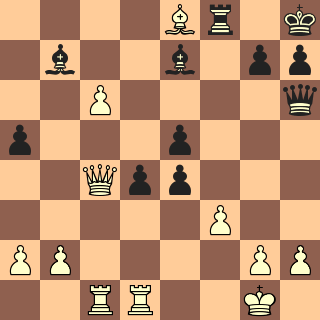
\includegraphics[scale=0.5]{fig/diagram_feat}
\caption[Chess Position]{chess position coming out of the game \textit{Alexander McDonnell vs Louis Charles Mahe De La Bourdonnais, London 1834} after 24. c6}
\label{fig:feat}
\end{figure}

\begin{table}[]
\centering
\begin{tabular}{c c c | c c c}
\toprule
\textbf{piece} & \textbf{piece map} & \textbf{mobility map} & \textbf{piece} & \textbf{piece map} & \textbf{mobility map} \\
\midrule

\includegraphics[scale=0.5]{fig/pieces/K} & 
$ \begin{smallmatrix} 0&0&0&0&0&0&0&0\\0&0&0&0&0&0&0&0\\0&0&0&0&0&0&0&0\\0&0&0&0&0&0&0&0\\0&0&0&0&0&0&0&0\\0&0&0&0&0&0&0&0\\0&0&0&0&0&0&0&0\\0&0&0&0&0&0&1&0 \end{smallmatrix} $ &  $\begin{smallmatrix}0&0&0&0&0&0&0&0\\0&0&0&0&0&0&0&0\\0&0&0&0&0&0&0&0\\0&0&0&0&0&0&0&0\\0&0&0&0&0&0&0&0\\0&0&0&0&0&0&0&0\\0&0&0&0&0&1&0&0\\0&0&0&0&0&1&0&1\end{smallmatrix}$  &


\includegraphics[scale=0.5]{fig/pieces/k} &
$\begin{smallmatrix}0&0&0&0&0&0&0&1\\0&0&0&0&0&0&0&0\\0&0&0&0&0&0&0&0\\0&0&0&0&0&0&0&0\\0&0&0&0&0&0&0&0\\0&0&0&0&0&0&0&0\\0&0&0&0&0&0&0&0\\0&0&0&0&0&0&0&0\end{smallmatrix}$ &
$\begin{smallmatrix}0&0&0&0&0&0&0&0\\0&0&0&0&0&0&0&0\\0&0&0&0&0&0&0&0\\0&0&0&0&0&0&0&0\\0&0&0&0&0&0&0&0\\0&0&0&0&0&0&0&0\\0&0&0&0&0&0&0&0\\0&0&0&0&0&0&0&0\end{smallmatrix}$ \\ [1cm]


\includegraphics[scale=0.5]{fig/pieces/Q} & 
$\begin{smallmatrix}0&0&0&0&0&0&0&0\\0&0&0&0&0&0&0&0\\0&0&0&0&0&0&0&0\\0&0&0&0&0&0&0&0\\0&0&1&0&0&0&0&0\\0&0&0&0&0&0&0&0\\0&0&0&0&0&0&0&0\\0&0&0&0&0&0&0&0\end{smallmatrix}$ &
$\begin{smallmatrix}0&0&0&0&0&0&1&0\\0&0&0&0&0&1&0&0\\1&0&0&0&1&0&0&0\\0&1&1&1&0&0&0&0\\1&1&0&1&0&0&0&0\\0&1&1&1&0&0&0&0\\0&0&1&0&1&0&0&0\\0&0&0&0&0&1&0&0\end{smallmatrix}$&


\includegraphics[scale=0.5]{fig/pieces/q} &
$\begin{smallmatrix}0&0&0&0&0&0&0&0\\0&0&0&0&0&0&0&0\\0&0&0&0&0&0&0&1\\0&0&0&0&0&0&0&0\\0&0&0&0&0&0&0&0\\0&0&0&0&0&0&0&0\\0&0&0&0&0&0&0&0\\0&0&0&0&0&0&0&0\end{smallmatrix}$ &
$\begin{smallmatrix}0&0&0&0&0&0&0&0\\0&0&0&0&0&0&0&0\\0&0&1&1&1&1&1&0\\0&0&0&0&0&0&1&1\\0&0&0&0&0&1&0&1\\0&0&0&0&1&0&0&1\\0&0&0&1&0&0&0&1\\0&0&1&0&0&0&0&0\end{smallmatrix}$ \\ [1cm]


\includegraphics[scale=0.5]{fig/pieces/R} & 
$\begin{smallmatrix}0&0&0&0&0&0&0&0\\0&0&0&0&0&0&0&0\\0&0&0&0&0&0&0&0\\0&0&0&0&0&0&0&0\\0&0&0&0&0&0&0&0\\0&0&0&0&0&0&0&0\\0&0&0&0&0&0&0&0\\0&0&1&1&0&0&0&0\end{smallmatrix}$ &
$\begin{smallmatrix}0&0&0&0&0&0&0&0\\0&0&0&0&0&0&0&0\\0&0&0&0&0&0&0&0\\0&0&0&0&0&0&0&0\\0&0&0&1&0&0&0&0\\0&0&1&1&0&0&0&0\\0&0&1&1&0&0&0&0\\1&1&0&0&1&1&0&0\end{smallmatrix}$ &

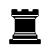
\includegraphics[scale=0.5]{fig/pieces/r} &
$\begin{smallmatrix}0&0&0&0&0&1&0&0\\0&0&0&0&0&0&0&0\\0&0&0&0&0&0&0&0\\0&0&0&0&0&0&0&0\\0&0&0&0&0&0&0&0\\0&0&0&0&0&0&0&0\\0&0&0&0&0&0&0&0\\0&0&0&0&0&0&0&0\end{smallmatrix}$ &
$\begin{smallmatrix}0&0&0&0&1&0&1&0\\0&0&0&0&0&1&0&0\\0&0&0&0&0&1&0&0\\0&0&0&0&0&1&0&0\\0&0&0&0&0&1&0&0\\0&0&0&0&0&1&0&0\\0&0&0&0&0&0&0&0\\0&0&0&0&0&0&0&0\end{smallmatrix}$ \\ [1cm]


\includegraphics[scale=0.5]{fig/pieces/B} & 
$\begin{smallmatrix}0&0&0&0&1&0&0&0\\0&0&0&0&0&0&0&0\\0&0&0&0&0&0&0&0\\0&0&0&0&0&0&0&0\\0&0&0&0&0&0&0&0\\0&0&0&0&0&0&0&0\\0&0&0&0&0&0&0&0\\0&0&0&0&0&0&0&0\end{smallmatrix}$&
$\begin{smallmatrix}0&0&0&0&0&0&0&0\\0&0&0&1&0&1&0&0\\0&0&0&0&0&0&1&0\\0&0&0&0&0&0&0&1\\0&0&0&0&0&0&0&0\\0&0&0&0&0&0&0&0\\0&0&0&0&0&0&0&0\\0&0&0&0&0&0&0&0\end{smallmatrix}$ &

\includegraphics[scale=0.5]{fig/pieces/b} &
$\begin{smallmatrix}0&0&0&0&0&0&0&0\\0&1&0&0&1&0&0&0\\0&0&0&0&0&0&0&0\\0&0&0&0&0&0&0&0\\0&0&0&0&0&0&0&0\\0&0&0&0&0&0&0&0\\0&0&0&0&0&0&0&0\\0&0&0&0&0&0&0&0\end{smallmatrix}$&
$\begin{smallmatrix}1&0&1&1&0&0&0&0\\0&0&0&0&0&0&0&0\\1&0&1&1&0&1&0&0\\0&0&1&0&0&0&1&0\\0&1&0&0&0&0&0&1\\1&0&0&0&0&0&0&0\\0&0&0&0&0&0&0&0\\0&0&0&0&0&0&0&0\end{smallmatrix}$ \\ [1cm]

\includegraphics[scale=0.5]{fig/pieces/N} &
$\begin{smallmatrix}0&0&0&0&0&0&0&0\\0&0&0&0&0&0&0&0\\0&0&0&0&0&0&0&0\\0&0&0&0&0&0&0&0\\0&0&0&0&0&0&0&0\\0&0&0&0&0&0&0&0\\0&0&0&0&0&0&0&0\\0&0&0&0&0&0&0&0\end{smallmatrix}$&
$\begin{smallmatrix}0&0&0&0&0&0&0&0\\0&0&0&0&0&0&0&0\\0&0&0&0&0&0&0&0\\0&0&0&0&0&0&0&0\\0&0&0&0&0&0&0&0\\0&0&0&0&0&0&0&0\\0&0&0&0&0&0&0&0\\0&0&0&0&0&0&0&0\end{smallmatrix}$ &

\includegraphics[scale=0.5]{fig/pieces/n} &
$\begin{smallmatrix}0&0&0&0&0&0&0&0\\0&0&0&0&0&0&0&0\\0&0&0&0&0&0&0&0\\0&0&0&0&0&0&0&0\\0&0&0&0&0&0&0&0\\0&0&0&0&0&0&0&0\\0&0&0&0&0&0&0&0\\0&0&0&0&0&0&0&0\end{smallmatrix}$ &
$\begin{smallmatrix}0&0&0&0&0&0&0&0\\0&0&0&0&0&0&0&0\\0&0&0&0&0&0&0&0\\0&0&0&0&0&0&0&0\\0&0&0&0&0&0&0&0\\0&0&0&0&0&0&0&0\\0&0&0&0&0&0&0&0\\0&0&0&0&0&0&0&0\end{smallmatrix}$ \\ [1cm]

\includegraphics[scale=0.5]{fig/pieces/P} &
$\begin{smallmatrix}0&0&0&0&0&0&0&0\\0&0&0&0&0&0&0&0\\0&0&1&0&0&0&0&0\\0&0&0&0&0&0&0&0\\0&0&0&0&0&0&0&0\\0&0&0&0&0&1&0&0\\1&1&0&0&0&0&1&1\\0&0&0&0&0&0&0&0\end{smallmatrix}$ &
$\begin{smallmatrix}0&0&0&0&0&0&0&0\\0&1&1&0&0&0&0&0\\0&0&0&0&0&0&0&0\\0&0&0&0&0&0&0&0\\1&1&0&0&1&1&1&1\\1&1&0&0&0&0&1&1\\0&0&0&0&0&0&0&0\\0&0&0&0&0&0&0&0\end{smallmatrix}$ &

\includegraphics[scale=0.5]{fig/pieces/p} &
$\begin{smallmatrix}0&0&0&0&0&0&0&0\\0&0&0&0&0&0&1&1\\0&0&0&0&0&0&0&0\\1&0&0&0&1&0&0&0\\0&0&0&1&1&0&0&0\\0&0&0&0&0&0&0&0\\0&0&0&0&0&0&0&0\\0&0&0&0&0&0&0&0\end{smallmatrix}$ &
$\begin{smallmatrix}0&0&0&0&0&0&0&0\\0&0&0&0&0&0&0&0\\0&0&0&0&0&0&1&0\\0&0&0&0&0&0&1&0\\1&0&0&0&0&0&0&0\\0&0&0&1&1&1&0&0\\0&0&0&0&0&0&0&0\\0&0&0&0&0&0&0&0\end{smallmatrix}$ \\

\bottomrule
\end{tabular}
\caption[Bitboards]{An example of how the chessboard from figure \ref{fig:feat} can be transformed to a stack of binary image channels}
\label{tab:feat}
\end{table}


\label{ex:feat}

Next to this, we can add additional (redundant) information to the features to help the model in question to learn patterns. Examples of additional features are
\begin{itemize}
\item side to move
\item indication for each castle if it is still possible
\item possibility to do en passant for each of the 16 squares where this could be a possibility
\item piece count for each piece type
\item piece mobility: number of squares each piece can go to
\item for each piece (type) the number of pieces it attacks
\item for each piece (type) the number of pieces it defends
\end{itemize}
We will call this data global features from now on. Some of these could be encoded with image maps as well. For example, every cell could denote the number of times it is attacked and defended.

\section{Static Evaluation Function}
\label{sec:sef}
In conventional chess engines, the heuristic evaluation function is linear, but also reinforcement learning chess programs often use a linear function: $V_w(s)=\sum w f(s)$ \cite{baxt99,veness09}. In this dissertation, we switch gears and use a neural network model instead, as they have the ability to model a larger range of functions and extract additional features from the data.\\
The chess engine \textit{Giraffe}, which uses a TD-learning algorithm, uses an \gls{fnn} architecture with 2 hidden layers \cite{giraffe15}. A totally different approach has been taken in \textit{DeepChess}, where the evaluation function is a deep siamese network learned on a big dataset of games between grandmasters. Two positions are given as input and the network returns which position is best. Playing is then performed with a comparison-based $\alpha\beta$-search. Admirably, \textit{DeepChess} succeeded at reaching a grandmaster level of play \cite{David2016}.\\

To our best knowledge, no one has experimented with a \gls{cnn} architecture to evaluate chess positions yet. The feature space presented in the previous section forms an intuitive basis to start with. The distinction between bitboard and global features demands for an architecture where the channel stack is the input of a \gls{cnn}, where some form of feature extraction is carried out. Next, the resulting feature maps are combined with the global feature vector into a \gls{fcn} with regression, as shown in figure \ref{fig:chessnetw}. 

\begin{figure}
\centering
\begin{tikzpicture}[scale=0.75]
%\draw[step=0.5cm,gray,very thin] (0,-4) grid (20,4);
\node (img) at (1,0) {\includegraphics[width=1.6cm]{fig/diagram_feat}};
\node at (-0.5,0) {$s$};
\draw (3,1.5) rectangle (5,3.5);
\draw (3.5,2) rectangle (5.5,4);
\draw (3.25,1.75) rectangle (5.25,3.75);
\draw[->] (1,1) -- (1,2.5) -- (3,2.5);
\draw (4,-1.5) rectangle (4.5,-4);
\draw[->] (1,-1) -- (1,-2.75) -- (4,-2.75);
\node at (4.25,1.25){bitboards};
\node at (3.25,-2.5){global};

\draw[->] (5.5,2.5) -- (7.5,2.5);
\draw (7.5,1.5) rectangle (10.5,3.5) node[pos=0.5,scale=2]{CNN};

\draw[->] (10.5,2.5) -- (12.5,2.5);
\draw (12.5,1.5) rectangle (14.5,3.5);
\draw (13,2) rectangle (15,4);
\draw (12.75,1.75) rectangle (14.75,3.75);
\node at (13.75,1.25){feature maps};

\draw[->] (15,2.5) -- (17,2.5);
\draw[->] (4.5,-2.75) -- (17,-2.75);
\draw[->] (17,-4) rectangle (18.5,4);
\node[scale=2.5] at (17.75,1.25) {F};
\node[scale=2.5] at (17.75,0) {C};
\node[scale=2.5] at (17.75,-1.25) {N};

\draw[->] (18.5,0) -- (20.5,0) node[pos=0.5,yshift=7.5pt]{$V(s)$};

%\node[staterect] (n0_0) at (0,0) {Agent} edge[mainedge, bend left] (n0_4);
%\node[staterect] (n0_4) at (0,-4) {Environment: $s_t$} edge[mainedge, bend left] (n0_0);
%\node at (-1,-2) {$a_t$};
%\node at (1.1,-2) {$r_{t+1}$};
%\node at (1.1,-2.5) {$s_{t+1}$};
\end{tikzpicture}
\caption[Network architecture value function]{Schematic overview of a possible network architecture for chess using CNNs}
\label{fig:chessnetw}
\end{figure}

\section{TD algorithms}
\label{sec:td}
As investigated in section \ref{subsec:vp}, TD algorithms are ideal in a \acrlong{ml} framework, because of its natural embedding of the optimization of the \gls{mse} cost function in its update rule. We saw that a TD($\lambda$) approach is often the best choice, as it combines the best of both \gls{mc} methods and classical \gls{td}-learning. We shortly review \gls{td}($\lambda$) in section \ref{subsec:tdy} and analyze its shortcomings, after which we consider alternatives using both the ideas of \gls{td}($\lambda$) and minimax search (for which it is of course more efficient to apply the $\alpha\beta$-search). These methods slightly differ in terms of the episodic weight updates.\\

Before we continue, we need to revise the \gls{rl} framework. In literature, the \gls{rl} framework for boardgames is often a simplification of the classical one represented in section \ref{sec:rl}. The reward function $r:\mathcal{S}\times\mathcal{A}\mapsto \mathbb{R}$ in boardgames is often chosen to be
\begin{equation}
\label{eq:reward}
r(s_t,a_t) = \begin{cases} 
   W(s_{t+1}) & \text{if } s_{t+1} \textnormal{ is terminal} \\
   0 & \text{if } \textnormal{else}
  \end{cases}
\end{equation}
where $W(s_{t+1})$ denotes the objective evaluation of the terminal state of the game (do not confuse with the static evaluation function). For chess, this objective evaluation can be (assuming $s$ is a terminal state)
\begin{equation}
W(s) = \begin{cases} 
   1 & \text{win} \\
   0 & \text{draw} \\
   -1 & \text{loss} \\
  \end{cases}
\end{equation}
Notice how this definition of the reward function meets the zero sum property. \\
Previous research in \gls{rl} in games mainly do not take the discount factor into account when performing a TD-learning. This is rationalized by considering the return $\mathcal{R}=\sum_{t=0}^{T}\gamma^t r(s_t,a_t)$. As $r(s_t,a_t)$ is zero everywhere except at the final state, it may be beneficial to assign the final reward as the return of every action, especially in \gls{td}-learning algorithms. The reason for this is a remark made in section \ref{subsec:vp} about the otherwise slow convergence properties in chaining.\\

In what follows, we will consider two main ideas to compute a target:
\begin{itemize}
\item episodic updates of the weights. After each episode the weights can be updated with an update rule. We could say this is a way of doing incremental learning over episodes. Here it is important to notice that the updates are heavily correlated, which may be the cause of bad generalization if we were to use them incrementally. The update rules make use of the assumptions about the simplified reward function and neutralized discount factor.
\item translation to supervised learning framework. What is needed, are a set of tuples $(s,\mathcal{R})$ where the return operates as a target value to learn $V(s)$. By using this approach, we can choose our favorite supervised learning algorithm from section \ref{subsubsec:ann}. We can gather these tuples over the course of many episodes and shuffle them before applying mini-batch \gls{sgd} (which is in general beneficial for the performance in software implementations) to improve generalization. 
\end{itemize}

\subsection{TD($\lambda$)}
\label{subsec:tdy}
\gls{td}($\lambda$) was the first \gls{rl} algorithm that proved to effective for learning to play a game. \textit{TD-Gammon} used a \acrlong{nn} with one fully connected sigmoidal hidden layer to learn a value function for backgammon \cite{tdgammon95}. Assume from now on  

\begin{equation}
V_{est}(s_t)=\begin{cases} 
   r_t &  \text{if } t=T \\
   \hat{V}(s_t) & \text{else} \\
  \end{cases}
\end{equation}

Under the conditions $\gamma=0$ and equation \ref{eq:reward} the temporal difference is defined to be

\begin{equation}
\label{eq:td}
\delta_t=V_{est}(s_{t+1})-V_{est}(s_{t})
\end{equation}

If we use a learning rate $\alpha$, we can now update the parameters after each episode with a history $(s_0,a_0,r_1),(s_1,a_1,r_2), \dotso , (s_{T-1},a_{T-1},r_T)$ as follows:

\begin{equation}
\label{eq:update}
w \leftarrow w-\alpha \sum_{t=0}^{T-1} \nabla_w V_{est}(s_t) \sum_{n=t}^{T-1} \lambda^{n-t}\delta_n
\end{equation}

This is equivalent to an episodic gradient descent update minimizing the \gls{mse} with the $\lambda$-return as target in supervised learning context. Remember that the general regression supervised learning paradigm can be summarized for a target $z$ with the formula

\begin{equation}
\bigtriangleup w =\alpha \nabla_w V_{est}(s_t) (z_t-V_{est}(s_t))
\end{equation}

Over the course of an episode $\left[s_0,r_1,s_1,\dotso,r_T,s_T\right]$, the total update amounts to
\begin{equation}
\bigtriangleup w =\alpha \sum_{t=0}^{T-1} \nabla_w V_{est}(s_t) (z_t-V_{est}(s_t))
\end{equation}
Hence, if equation \ref{eq:update} were a gradient descent update, following equality should hold:
\begin{equation}
z_t-V_{est}(s_t) = \sum_{n=t}^{T-1} \lambda^{n-t}\delta_n
\end{equation}
Working this out yields
\begin{align*}
z_t &=\sum_{n=t}^{T-1} \lambda^{n-t} \left[V_{est}(s_{n+1})-V_{est}(s_{n})\right]+V_{est}(s_t) \\
&= \quad \quad \lambda^0\left[V_{est}(s_{t+1}-V_{est}(s_t))\right] \\
& \quad \quad+\lambda\left[V_{est}(s_{t+2}-V_{est}(s_{t+1}))\right] \\
& \quad \quad+ \dotso\\
& \quad \quad +\lambda^{T-1-t}\left[V_{est}(s_{T}-V_{est}(s_{T-1}))\right] + V_{est}(s_T) \\
&= \sum_{n=0}^{T-2-t}(\lambda^n-\lambda^{n+1})V_{est}(s_{t+1+n}) \lambda^{T-1-t}V_{est}(s_T)\\
&= (1-\lambda)\sum_{n=1}^{T-1-t}\lambda^{n-1}V_{est}(s_{t+n}) + \lambda^{T-1-t}V_{est}(s_T)\\
&= (1-\lambda)\sum_{n=1}^{T-1-t}\lambda^{n-1}V_{est}(s_{t+n}) + \lambda^{T-1-t}(1-\lambda)V_{est}(s_T)+ \lambda^{T-t}V_{est}(s_T)\\
&= (1-\lambda)\sum_{n=1}^{T-t}\lambda^{n-1}V_{est}(s_{t+n}) + \lambda^{T-t}V_{est}(s_T)\\
\end{align*}
Combining the defined reward function, $\gamma=1$ and equation \ref{eq:nstep} for the n-step return, we notice how the n-step return is equal to the approximated value function n steps ahead: $G_n(s_t)=V_{est}(s_{t+n})$. The return after the terminal state is trivially estimated to be the value function at the terminal state: $V(s_T)$. Hence we achieve (using equation \ref{eq:tdlambda_fin}) our final result
\begin{align}
z_t&=(1-\lambda)\sum_{n=0}^{T-t}\lambda^{n-1}G_n(s_t) + G_t\\
&=G_\lambda(s_t)
\end{align}

The amazing thing about \textit{TD-Gammon} is that its level surpassed that of humans by using strategies that were considered bad at that time. These techniques were later incorporated into humans play. One characteristic about its evaluations was that objectively better positions were estimated a smaller value than worse positions. Still, the engine was able to choose the best move. \textit{Tesauro} explains this by the huge similarity between consecutive positions for the neural network, resulting in a smaller difference. For choosing the right move, the relative error is much more important than the absolute error.\\
Another key to the success of \textit{TD-Gammon} is the stochasticity of the game. Thanks to the stochastic noise the agent is able to discover new strategies much quicker than it would in a deterministic environment.\\

In section \ref{subsec:vp} a supervised learning algorithm using $z_t$ as target was laid out. It is key to remember that the update rule from equation \ref{eq:update} is essentially a supervised learning regression algorithm, but generalizing for $G_lambda(s_t)$ may be beneficial, as we can study the influence of the discount factor and reward function in this manner. To resume and summarize, the target values for the network are equal to

\begin{equation}
G_\lambda(s_t) = (1-\lambda) \sum_{n=1}^{T-t} \lambda^{n-1} \left[\sum_{i=0}^{n-1} \left( \gamma^i r_{k+i}\right) + \gamma^n V_{est}(s_{k+n}) \right]
\end{equation}

in the standard TD($\lambda$) method. The techniques from the following sections will only differ in how we define our target $z_t=G_\lambda(s_t)$.\\
Algorithm \ref{al:sltd} is the supervised learning framework, independent of the definition of $z_t$, hence independent of the implemented \gls{td} algorithm and conditions. It consists of following noteworthy elements:
\begin{itemize}
\item random initialization of the network's parameters.
\item playing episodes with the current network under some policy. Let us assume it is $\epsilon$-greedy for now.
\item calculating the matching returns from all played games and adding the tuples $(s_t,z_t)$ to replay memory $\mathcal{D}$. In algorithm \ref{al:sltd} the replay memory gets refreshed every iteration, but more sophisticated methods to have a representable dataset may be applied.
\item splitting $\mathcal{D}$ in a training set $\mathcal{D}_{training}$ and validation set $\mathcal{D}_{test}$
\item doing experience replay: random sampling of minibatches from $\mathcal{D}$, from which the weights will be updated with gradient descent.
\item learn until the loss on the validation set stops decreasing, to avoid the network from overfitting.
\end{itemize}

\begin{algorithm}
\begin{algorithmic}
	\STATE Initialize $w$ (randomly)
	\REPEAT
		\STATE play $N$ episodes $\rightarrow (\mathcal{H}_1,\dotso,\mathcal{H}_N)$
		\STATE $\mathcal{D}=\{\}$
		\COMMENT{create a dataset to store experience from episodes}
		\FOR {$i\leftarrow 1$ to $N$}
			\FOR {$s_t \in \mathcal{H}_i$}
				\STATE$\mathcal{D} \leftarrow \mathcal{D} \cup \{(s_t,z_t)\}$
				\COMMENT{calculate return}
			\ENDFOR
		\ENDFOR
		\STATE shuffle samples
		\STATE select $\mathcal{D}_{training}$ and $\mathcal{D}_{test}$ from  $\mathcal{D}$
		\REPEAT		
			\FOR{all minibatches $\in \mathcal{D}_{training}$}
				\STATE $w \gets w-\alpha\sum_{i=1}^{n}\frac{\nabla L_i(w)}{n}$
			\ENDFOR
		\UNTIL loss on $\mathcal{D}_{test}$ stops decreasing
	\UNTIL satisfying convergence
\end{algorithmic}
\caption{supervised TD algorithm}
\label{al:sltd}
\end{algorithm}

If we were to implement TD($\lambda$) onto the chess model, it would be hard for the agent to learn to play well. This is due to these main reasons:
\begin{itemize}
\item in contrast to backgammon, chess is a deterministic game, which will make exploration harder under a non adapted policy
\item chess is a very tactical game. This fact requires some sort of tree search. With TD($\lambda$) we are only looking one move ahead under an $\epsilon$-greedy policy.
\end{itemize}
The policy problem is somewhat hard to solve (we will look further into it in section \ref{sec:polnet}), but we can introduce tree search in different fashions as we will see next. 

\subsection{TD-directed($\lambda$)}
\label{subsec:tddir}
This is the easiest minimax variant proposed by the developers of \textit{KnightCap} \cite{baxt99}. The same update rules and target are applied as in TD($\lambda$). The one difference lies in the policy. Play is guided by the minimax value at a depth $d$.

\subsection{TD-root($\lambda$)}
\label{subsec:tdroot}
A first algorithm introducing a minimax search into TD-learning is TD-root($\lambda$), its idea already dates back to 1959(!), where the agent was able to reach an amateur level in checkers \cite{samuel59}. The idea is to update the value functions in positions into the direction of the minimax values, as they are better representation of the actual value at that state, as shown in figure \ref{fig:tdroot}. By doing this, the values at states will have the tree search incorporated into it. The value at the roots change into the direction of the values at the leafs of the principal variations.\\
To continue, we define the function $l:\mathcal{S} \times \mathbb{N}_{>0}\mapsto\mathcal{S}$ that projects a state to its leaf state given a depth following the path of the \acrlong{pv}. To incorporate this idea into \gls{td} learning, we only need to slightly modify equation \ref{eq:td} for a certain depth $d$ to 
\begin{equation}
\label{eq:tdroot}
\delta_t=V_{est}\left(l(s_{t+1},d)\right)-V_{est}(s_{t})
\end{equation}
The update rule with the simplified conditions and TD-error from equation \ref{eq:tdroot} is then equation \ref{eq:update}. The corresponding target value for every state is consequently
\begin{equation}
z_t=\sum_{n=t}^{T-1} \lambda^{n-t} \delta_n+V_{est}(s_T)
\end{equation}

\begin{figure}
\centering
\begin{tikzpicture}[scale=0.9]
%\draw[step=1cm,gray,very thin] (-8,-2) grid (8,4);
\node[state,fill=black] (s0) at (-5,4){} ;
\node[state] (s1) at (-7,2){} edge[mainedge,dashed] (s0);
\node[state] (s2) at (-3,2){} edge[mainedge] (s0);
\node[state] (s3) at (-8,0){} edge[mainedge,dashed] (s1);
\node[state] (s4) at (-6,0){} edge[mainedge,dashed] (s1);
\node[state] (s5) at (-4,0){} edge[mainedge] (s2);
\node[state] (s6) at (-2,0){} edge[mainedge,dashed] (s2);
\node at (-5,-1){$t$};

\draw[dashed] (0,-1) -- (0,5);

\node[state,fill=blue] (t0) at (5,4){};
\node[state] (t1) at (7,2){} edge[mainedge,dashed] (t0);
\node[state] (t2) at (3,2){} edge[mainedge] (t0);
\node[state] (t3) at (8,0){} edge[mainedge,dashed] (t1);
\node[state] (t4) at (6,0){} edge[mainedge,dashed] (t1);
\node[state] (t5) at (4,0){} edge[mainedge,dashed] (t2);
\node[state,fill=red] (t6) at (2,0){} edge[mainedge] (t2);
\node at (5,-1){$t+1$};

\node[state] (s0) at (-5,4){} edge[mainedge,color=red,bend left] node[midway,xshift=-0.5cm,yshift=-0.5cm]{TD-root($\lambda$)} (t6) edge[mainedge,color=blue,bend left=10] node[midway,yshift=-0.5cm]{TD($\lambda$)} (t0);

\end{tikzpicture}
\caption[Comparison between TD-root($\lambda$) and TD($\lambda$)]{Comparison between TD-root($\lambda$) and TD($\lambda$). In TD($\lambda$), the root nodes get feedback (an error signal) from the root at the next time step, while in TD-root($\lambda$), the root receives its feedback signal from the principal leaf node at the next state.}
\label{fig:tdroot}
\end{figure}

\subsection{TD-leaf($\lambda$)}
\label{subsec:tdleaf}
An issue with TD($\lambda$) and TD-root($\lambda$) is that they only update according the line of play, which correlates the data. By using the same minimax idea as before, but now updating the leaf along the \gls{pv} to the leaf along the \gls{pv} of the next position, we obtain data from positions not played. This is because the \gls{pv} up until a certain depth is not necessarily the same path as in the following position. This idea is named TD-leaf($\lambda$), and was used to train against expert chess opponents in \textit{KnightCap} and \textit{Giraffe} \cite{baxt99,giraffe15}. Also with TD-leaf($\lambda$), a superhuman level in checkers has been achieved \cite{chinook}. The update rule is depicted at figure \ref{fig:tdleaf}. \\
The temporal difference and corresponding update rule defining this update are
\begin{align}
\delta_t&=V_{est}\left(l(s_{t+1},d)\right)-V_{est}(l(s_{t},d))\\
w &\leftarrow w-\alpha \sum_{t=0}^{T-1} \nabla_w V_{est}(l(s_t,d)) \sum_{n=t}^{T-1} \lambda^{n-t}\delta_n
\end{align}
Hence, our tuple for our supervised learning framework consists out of $l(s_t)$ and
\begin{equation}
z_t=\sum_{n=t}^{T-1} \lambda^{n-t} \delta_n+V_{est}(l(s_T,d))
\end{equation}
which analogously as in section \ref{subsec:tdy} can be transformed to
\begin{align}
z_t&=(1-\lambda)\sum_{n=0}^{T-t}\lambda^{n-1}V_{est}(l(s_{t+n},d)) + \lambda^{T-t}V_{est}(s_T)\\
&=G_\lambda(s_t)
\label{eq:leafreturn}
\end{align}
using the property that the leaf of a terminal state is itself, or put otherwise $l(s_T)=s_T$. With equation \ref{eq:leafreturn}, we can define the $\lambda$-return for general discount rates and reward functions.
The attentive reader noticed it was impossible to generalize the target to $G_\lambda(s_t)$ for TD-root($\lambda$), because factors can not be canceled out when comparing leaves to roots.

\begin{figure}
\centering
\begin{tikzpicture}[scale=0.9]
%\draw[step=1cm,gray,very thin] (-8,-2) grid (8,4);
\node[state] (s0) at (-5,4){} ;
\node at (-4.25,4){$s_t$};
\node[state] (s1) at (-7,2){} edge[mainedge,dashed] (s0);
\node[state] (s2) at (-3,2){} edge[mainedge] (s0);
\node at (-2.125,2){$s_{t+1}$};
\node[state] (s3) at (-8,0){} edge[mainedge,dashed] (s1);
\node[state] (s4) at (-6,0){} edge[mainedge,dashed] (s1);
\node[state,fill=black] (s5) at (-4,0){} edge[mainedge] (s2);
\node[state] (s6) at (-2,0){} edge[mainedge,dashed] (s2);
\node at (-5,-1){$t$};

\draw[dashed] (0,-1) -- (0,5);

\node[state] (t0) at (5,4){};
\node at (5.875,4){$s_{t+1}$};
\node[state] (t1) at (7,2){} edge[mainedge,dashed] (t0);
\node[state] (t2) at (3,2){} edge[mainedge] (t0);
\node[state] (t3) at (8,0){} edge[mainedge,dashed] (t1);
\node[state] (t4) at (6,0){} edge[mainedge,dashed] (t1);
\node[state] (t5) at (4,0){} edge[mainedge,dashed] (t2);
\node[state,fill=black] (t6) at (2,0){} edge[mainedge] (t2);
\node at (5,-1){$t+1$};

\node[state] (s0) at (-4,0){} edge[mainedge,color=black,bend right=20] node[midway,yshift=-0.5cm]{TD-leaf($\lambda$)} (t6);

\end{tikzpicture}
\caption[TD-leaf($\lambda$)]{How updates in TD-leaf($\lambda$) work. The \gls{pv}s are denoted by the non dashed paths in the search tree. Notice how the paths may be different in the next state. The updates happen from leaf to leaf, which not necessary need to be played.}
\label{fig:tdleaf}
\end{figure}

\subsection{TD-stem($\lambda$)}
\label{subsec:tdrootleaf}
To conclude this section about TD algorithms, we will examine an own contribution (to the best of our knowledge): TD-stem($\lambda$). The idea is to simply combine the ideas of TD-leaf($\lambda$) and TD-root($\lambda$) by defining the error as the difference between the leaves, but updating the root state. This makes sense, as it seems to annihilate disadvantages of the former methods. In TD-leaf($\lambda$) the update can be from another path (resulting in being erroneous), while TD-root($\lambda$) can not be generalized to a $\lambda$-return. Essentially, the update is in the direction of the error between the minimax values of consecutive states. An additional bonus could be the incorporation of depth into the static evaluation function. However, this could also be a disadvantage, as this could make the evaluation more noisy. the main idea is depicted in \ref{fig:tdrootleaf}. \\
To formalize this idea into mathematics:
\begin{align}
\delta_t&=V_{est}\left(l(s_{t+1},d)\right)-V_{est}(l(s_{t},d))\\
w &\leftarrow w-\alpha \sum_{t=0}^{T-1} \nabla_w V_{est}(s_t) \sum_{n=t}^{T-1} \lambda^{n-t}\delta_n
\end{align}
The generalization to $\lambda$-return is straightforward, with retrospect to equation \ref{eq:leafreturn}.

\begin{figure}
\centering
\begin{tikzpicture}[scale=0.9]
%\draw[step=1cm,gray,very thin] (-8,-2) grid (8,4);
\node[state,fill=black] (s0) at (-5,4){} ;
\node at (-4.25,4){};
\node[state] (s1) at (-7,2){} edge[mainedge,dashed] (s0);
\node[state] (s2) at (-3,2){} edge[mainedge] (s0);
\node at (-2.125,2){};
\node[state] (s3) at (-8,0){} edge[mainedge,dashed] (s1);
\node[state] (s4) at (-6,0){} edge[mainedge,dashed] (s1);
\node[state,fill=black] (s5) at (-4,0){} edge[mainedge] (s2);
\node[state] (s6) at (-2,0){} edge[mainedge,dashed] (s2);
\node at (-5,-1){$t$};

\draw[dashed] (0,-1) -- (0,5);

\node[state] (t0) at (5,4){};
\node at (5.875,4){};
\node[state] (t1) at (7,2){} edge[mainedge,dashed] (t0);
\node[state] (t2) at (3,2){} edge[mainedge] (t0);
\node[state] (t3) at (8,0){} edge[mainedge,dashed] (t1);
\node[state] (t4) at (6,0){} edge[mainedge,dashed] (t1);
\node[state] (t5) at (4,0){} edge[mainedge,dashed] (t2);
\node[state,fill=black] (t6) at (2,0){} edge[mainedge] (t2);
\node at (5,-1){$t+1$};

\node[state] (s0) at (-4,0){} edge[mainedge,color=black,bend right=20](t6);
\node[state] (s1) at (-5,4){} edge[mainedge,color=black] node[midway,xshift=-0.9cm,yshift=-0.5cm]{TD-stem($\lambda$)} (s0);

\end{tikzpicture}
\caption[TD-stem($\lambda$)]{In TD-stem($\lambda$), the root is updated based on values of the consecutive leaf node values.}
\label{fig:tdrootleaf}
\end{figure}

\section{Bootstrapping Tree Search}
\label{sec:bts}
There are three drawbacks to the TD algorithms with search included discussed in previous section:
\begin{enumerate}
\item Only one node gets updated for every tree search, making the search somewhat inefficient.
\item The positions may not be representative or too coherent with each other, as they are all based on actual occurrences or computed best line of play (\gls{pv}).
\item The target search is based on move played. Hence, this method is much more effective when the player is already strong.
\end{enumerate}
Especially the third point is a major turn off in our point of view, as we want to inject as less expert domain knowledge as possible into our model.\\
To address these problems, we could make more samples by using all information we got from the tree search. Additionally, we do not use the search from future, but rather use the minimax value directly as target. These ideas have been implemented in the chess engine \textit{Meep}, reaching an expert rating with self play \cite{veness09}.

%
%\subsection{Rootstrap($\lambda$)}
%\label{subsec:rootstrap}
%In rootstrap, the supervised learning framework can be used. The tuple consists out of the state from self-play $s_t$ and the estimated value at the leaf node:
%\begin{equation}
%z_t=V_{est}(l(s_t))
%\end{equation}
%This is the way it was implemented in \textit{Meep}, but we can actually generalize this to also include temporal knowledge into our target by using ideas from \gls{td} learning as we have seen in section \ref{sec:td} in the following way:
%\begin{align}
%\delta_t&=V_{est}(l(s_t,d))-V_{est}(s_t) \\
%z_t&=\sum_{n=t}^{T-1} \lambda^{n-t} \delta_n+V_{est}(l(s_T,d))
%\end{align}
%The corresponding change of the parameters over the course of an episode would then be
%\begin{equation}
%\bigtriangleup w =\alpha \sum_{t=0}^{T-1}\nabla_w V_{est}(s_t) \sum_{n=t}^{T-1} \lambda^{n-t} \delta_n
%\end{equation}
%By reformulating this equation
%\begin{align*}
%\bigtriangleup w &=\alpha \sum_{t=0}^{T-1}\nabla_w V_{est}(s_t) \sum_{n=t}^{T-1} \lambda^{n-t} \left[V_{est}(l(s_n,d))-V_{est}(s_{n+1})\right] \\
%&= \alpha \sum_{n=0}^{T-1} \left[V_{est}(l(s_n,d))-V_{est}(s_{n+1})\right] \sum_{t=0}^{n} \lambda^{n-t} \nabla_w V_{est}(s_t)
%\end{align*}
%we gain the insight that using this target function will result in prioritizing the differences closer to the end of the episode. This could potentially be advantageous, as it is hard to tell from the start through self play without expert initialization how good states at the start from the game are, and looking at a shallow depth will not help at the start. By using exponential weights we can insert more depth to the updates.
%
%
%\subsection{Treestrap($\lambda$)}
%\label{subsec:treestrap}
%So far, we have only added one sample to the dataset after each search. Treestrap, implemented for \textit{Meep} solves this issue by not discarding any gained information and adding tuples for each node in the search tree to the dataset. The deeper the node resides in the tree, the lower the depth information from minimaxing. Here, it is harder to add the idea of the exponential weights, as we update along lines we will never have seen, although it is still possible along the played lines. This is what we will call treestrap($\lambda$).
%
%\begin{figure}
%\centering
%\begin{tikzpicture}[scale=0.9]
%%\draw[step=1cm,gray,very thin] (-8,-2) grid (8,4);
%\node[state,fill=blue] (s0) at (-5,4){} ;
%\node at (-4.25,4){};
%\node[state,fill=red] (s1) at (-7,2){} edge[mainedge,dashed] (s0);
%\node[state,fill=red] (s2) at (-3,2){} edge[mainedge] (s0);
%\node at (-2.125,2){};
%\node[state,fill=red] (s3) at (-8,0){} edge[mainedge] (s1);
%\node[state] (s4) at (-6,0){} edge[mainedge,dashed] (s1);
%\node[state,fill=blue] (s5) at (-4,0){} edge[mainedge] (s2);
%\node[state] (s6) at (-2,0){} edge[mainedge,dashed] (s2);
%\node at (-5,-1){$t$};
%
%\draw[dashed] (0,-1) -- (0,5);
%
%\node[state,fill=blue] (t0) at (5,4){};
%\node at (5.875,4){};
%\node[state,fill=red] (t1) at (7,2){} edge[mainedge,dashed] (t0);
%\node[state,fill=red] (t2) at (3,2){} edge[mainedge] (t0);
%\node[state,fill=red] (t3) at (8,0){} edge[mainedge] (t1);
%\node[state] (t4) at (6,0){} edge[mainedge,dashed] (t1);
%\node[state] (t5) at (4,0){} edge[mainedge,dashed] (t2);
%\node[state,fill=blue] (t6) at (2,0){} edge[mainedge] (t2);
%\node at (5,-1){$t+1$};
%
%%\node[state] (s0) at (-4,0){} edge[mainedge,color=black,bend right=20](t6);
%\node[state] (s0) at (-5,4){} edge[mainedge,color=blue] (s5);
%\node[state] (s1) at (-3,2){} edge[mainedge,bend left,color=red] (s5);
%\node[state] (s2) at (-7,2){} edge[mainedge,bend right,color=red] (s3);
%
%\node[state] (t0) at (5,4){} edge[mainedge,color=blue,bend right=45] (t6);
%\node[state] (t2) at (3,2){} edge[mainedge,bend left,color=red] (t6);
%\node[state] (t1) at (7,2){} edge[mainedge,bend left,color=red] (t3);
%
%\end{tikzpicture}
%\caption{The rootstrap updates are colored blue. The additional treestrap updates are depicted in red. In this example, we gain thrice as much samples for the same search by using treestrap. Notice how the algorithms do not use the search values from the next state, in contrast to TD learning methods.}
%\label{fig:rootstrap}
%\end{figure}

\section{Monte Carlo Tree Search}
\label{sec:mcts}
We briefly look into a \gls{rl} method,  that has been proven to be widely successful, especially in Go, but from which the application to chess seems to be a hard nut to crack. It is an algorithm where researchers can show off their creativity by extending the basic methodology, which is why we should not deaden its potential contribution to chess. Because the \textit{AlphaGo} paper is a huge influence for this master thesis, we will investigate its \gls{mcts} implementation a little more in detail.\\
The basic idea is simple, by building a search tree in an asymmetric manner we optimally try to balance out exploitation and exploration. The search tree is expanded along simulations, from which the final result is propagated back into earlier encountered search nodes. These final results have an impact on the future search. \\ 
The base algorithm consists out of four phases for each iteration as also illustrated in figure \ref{fig:mcts} \cite{browne12}:
\begin{enumerate}
\item \textbf{Selection}. starting from the root state, a tree policy is followed to branch through the tree until arriving at a (current) leaf node. One important characteristic about the tree policy is its exploration exploitation balance by embedding the state visit
\item \textbf{Expansion}. an additional node is added to the search tree with the tree policy
\item \textbf{Simulation}. from the expanded node on, a \gls{mc} roll-out with a default policy is performed until arriving at a final state.
\item \textbf{Backpropagation}. the final result of the simulation is used to update statistics and values of the nodes in the search tree
\end{enumerate}
Typically, these phases are executed iteratively until a certain computational budget has been reached. At this point the final decision about the next action is returned.

\begin{figure}
\includegraphics[width=\linewidth]{fig/mcts}
\caption[\gls{mcts}]{Illustration of how \gls{mcts} algorithms function.}
\label{fig:mcts}
\end{figure}

The main things this method tries to achieve are to approximate the value of actions through random simulations and to use values efficiently for a best-first strategy. While the agent in TD algorithms tries to learn a long term value for each state, its purpose in \gls{mcts} is to estimate temporary state values to decide the play of the next move. In this respect, it is an algorithm competing with $\alpha\beta$-search for deciding the next move. In general, minimax is considered to be an unsuitable choice if no reliable heuristic exists. For large branch factors \gls{mcts}'s ideas are also superior to minimax, as it is easier to gain depth. However, it is argued that \gls{mcts} performs poorly in tactical situations where the smallest mistake may be decisive \cite{rama11}. These considerations lead to the insight that it may be hard for \gls{mcts} to improve chess play, especially in comparison with minimax. On the other hand, as we are trying to assume no additional domain specific knowledge, the simulation aspect of \gls{mcts} could help things out. It feels like more research into this topic needs to be conducted.

\subsection{AlphaGo}
Here, we discuss how a \gls{mcts} algorithm has been implemented in \textit{AlphaGo}, as it may gain more insight how it could be beneficial to self play in a \gls{rl} game environment \cite{alphago16}.
The phases are constructed in the following way (figure \ref{fig:alphago}):
\begin{enumerate}
\item \textbf{Selection}. Each edge contains statistics about the results obtained previously under the tree and roll-out policy. The stored values for an edge corresponding with the action $a$ from state $s$ are the action value $Q(s,a)$, the visit count (the number of iteration passing through that node) $N(s,a)$ and a prior probability $P(s,a)$ representing the policy learned with a policy network, see section \ref{sec:polnet}. The tree policy for the selection phase is then defined to be
\begin{equation}
a_t=\text{argmax}_{a}\left\{Q(s_t,a_t)+u(s_t,a_t)\right\}
\end{equation}
where $u(s_t,a_t)\propto\frac{P(s,a)}{1+N(s,a)}$, hence $u(s,a)$ encourages exploration.
\item \textbf{Expansion.} From the leaf node on, the default policy (a faster version of the previous described network) is applied. If the child of the leaf has been visited a sufficient number of times, it will be added to search tree.
\item \textbf{Simulation.} A \gls{mc} roll-out yields the final result $r$ of the game under the default policy. 
\item \textbf{Backpropagation.} The value that will be propagated back to through the edges of the tree is
\begin{equation}
V(s_L)=(1-\mu)\hat{V}(s_L)+\mu r
\end{equation}
where $\hat{V}(s_L)$ is the estimation by feeding the leaf node through the neural network. All edges through the path of the search tree are updated according to the following rule:
\begin{align}
N(s,a) & \leftarrow N(s,a)+1 \\
Q(s,a) & \leftarrow (1-\frac{1}{N(s,a)})Q(s,a)+\frac{1}{N(s,a)}V(s_L)
\label{eq:mcts_update}
\end{align}
\end{enumerate}
where equation \ref{eq:mcts_update} is a moving average over all encountered leaf values.

\begin{figure}
\includegraphics[width=\linewidth]{fig/alphago_mcts}
\caption[AlphaGo]{Illustration of the four phases of \gls{mcts} in \textit{AlphaGo}.}
\label{fig:alphago}
\end{figure}

\section{Policy Gradient Reinforcement Learning}
\label{sec:polnet}
Only approximating the value function has a big downside for deterministic games, namely that the smallest difference in value between two actions can cause a change in selection between moves \cite{sutton00}.
A common theme in learning to play games is to iterate between learning a value function and policy iteratively, as discussed in section \ref{subsec:iter}. For very large state spaces, which is the most common in game theory, this equals iterating between learning an approximation function $V_w(s)$ and a probability distribution $\pi_w(a|s)$. \\
Just as a deep neural network can be used to learn $V_w(s)$, the same is true for $\pi_w(a|s)$, where the difference in architecture between both is a softmax layer at the end instead of a single value learned with regression. Policy networks have proven their strengths in Go \cite{alphago16}.\\

Making policy networks a viable option for Go is the encoding of the actions, which is simply setting a stone at a certain square. Actions can thus easily be encoded with an output map. For chess, this encoding is much harder, as of al the legal actions possible in the game, at each state only a few are possible. An interesting research question is how policy networks can be incorporated into learning to play chess by finding decent encodings, especially for a CNN framework. A possible idea is the use of 2 output maps, one for the start position and one for the final position of a piece, hence encoding a uci move. This results in the encoding of $64^2$ actions, from which most of them are not legal, especially from a certain state where the average breadth is around 20. \\

Another potential idea is recent research into Atari games, where a new CNN architecture has been proposed to estimate the optimal advantage function, defined to be
\begin{equation}
A(s,a)=Q(s,a)-V(s)
\end{equation}
The dueling \gls{ddqn} learns $Q(s,a)$ by separately learning the advantage and the value in the same network. By estimating the advantage function, we can significantly reduce the variance on the policy, which is very state dependent, hence this network could be a better choice than separating with an individual policy network. The dueling \gls{ddqn} is the state of the art in playing Atari games \cite{dddqn15}.

\section{Monte Carlo Value Initialization}

All current \gls{rl} techniques in chess use some sort of expert knowledge for the time being. \textit{KnightCap} performed its training by playing humans and initializing its weights to piece value count, \textit{Giraffe} initialized its network weights in the same way and used grandmaster positions to start with. \textit{Meep} used handcrafted expert chess features. For the vision of this thesis, all these methods are forbidden, as they introduce some expert bias. At the same time, some initialization might be necessary to have a good point to start from and speed up training, as TD learning might take a very long time due to its nature to propagate back from the ending evaluation. The trick that made some of the previous chess engines quite successful was the initialization to a piece value count, as in this fashion, it is not necessary to branch out episodes up until the total end, the checkmate, which would be time consuming.\\

An own idea came to mind, trying to solve this issue. We will call the algorithm the \gls{mcvi}, as it heavily relies on \gls{mc} roll-outs. The idea is to set up random positions, and create a raw estimate of the value function based on the statistical results of the roll-out from that board position. As the statistics provide a value between 0 and 1, we transform it to be zero sum with the following equation:
\begin{equation}
V\leftarrow\frac{2w}{w+l}-1
\label{eq:v_mcvi}
\end{equation}
which provides as a number between -1 and 1, hence mimicking the optimal value function. As positions with less pieces are on average objectively closer to a terminal state with optimal play and easier to finish, we start off the algorithm with less pieces. After this, we can continue for more pieces and play until a certain confidence is reached over the positions by evaluating them through the network, as the network already learned how to handle these with raw evaluations for less pieces. This (obviously) saves out time, as we do not have to execute the simulations until a terminal state has reached, and stop preemptively. A rudimentary algorithm is depicted in \ref{al:mcvi}. \\
It is important to note how draws are not accounted in the calculations. We drop these simulations, as statistically speaking, by performing completely random actions without any peculiar policy, the relative difference between wins and losses would be minimized. The obtained values would not be a good indication about who got the better opportunities if play would be better.\\ 

\begin{algorithm}
\begin{algorithmic}
\REQUIRE $P,M,N$
\FOR{$i\leftarrow1$ to $P$}
	\STATE$\mathcal{D}\leftarrow\left\{\right\}$
	\FOR{$m\leftarrow1$ to $M$}
		\STATE{$B\leftarrow$ random position with $P$ pieces}
		\FOR{$n\leftarrow1$ to $N$}
			\STATE $w\leftarrow0$
			\STATE $l\leftarrow0$
			\STATE $r\leftarrow\text{MC-rollout}(B)$
			\COMMENT{until certain confidence from end result is reached}
			\IF{$r$ is a win}
				\STATE $w\leftarrow w+1$
			\ELSIF{$r$ is a loss}
				\STATE $l\leftarrow l+1$
			\ENDIF
		\ENDFOR
		\STATE $V\leftarrow\frac{2w}{w+l}-1$
		\STATE $\mathcal{D}\leftarrow\mathcal{D}\cup\left\{(B,V)\right\}$ 
	\ENDFOR
	\STATE fit $\mathcal{D}$ to network
\ENDFOR
\end{algorithmic}
\caption{Monte Carlo Value Initialization}
\label{al:mcvi}
\end{algorithm}

There are still some pitfalls that could ruin the joy:
\begin{itemize}
\item in some positions it is clear how play should continue, and how the side with the material advantage can win, but random play may benefit the other side. An example is illustrated in figure \ref{fig:mcvi1}.
\item Some positions are a draw, but random play may let the side that is the most probable to make a mistake do foolish actions, while the strategy maintaining the draw is straightforward (figure \ref{fig:mcvi2}).
\item To yield a good first rough estimate, many simulations may still be needed for every $P$.
\end{itemize}
We may hope, that these strange positions are exceptions, and that the law of big numbers may weaken their influence.

\begin{figure}
\centering
    \begin{subfigure}[t]{0.45\textwidth}
        \includegraphics[scale=0.5]{fig/diagram_mcvi}
        \caption{white is on the winning hand here, but black is more probable to win with random moves. The probability is sufficiently high that the black pawn will succeed at promoting to a queen, while setting the mating net is not straightforward to accomplice with the white pieces.}
        \label{fig:mcvi1}
    \end{subfigure}
    \qquad
    ~ %add desired spacing between images, e. g. ~, \quad, \qquad, \hfill etc. 
      %(or a blank line to force the subfigure onto a new line)
    \begin{subfigure}[t]{0.45\textwidth}
        \includegraphics[scale=0.5]{fig/diagram_mcvi2}
        \caption{To hold a draw, black can just move back and forward from a8 and b7. The problem is that black will make mistakes by playing randomly, and white will achieve an evaluation of 1 with equation \ref{eq:v_mcvi}.}
        \label{fig:mcvi2}
    \end{subfigure}
    ~ %add desired spacing between images, e. g. ~, \quad, \qquad, \hfill etc. 
    %(or a blank line to force the subfigure onto a new line)
    \caption{Two examples leading to bad $MC$ evaluations.}
\end{figure}

To conclude this section, let us make a final remark about our vision in this document. We assume the agent should know nothing more than the rules at the beginning of the game. If we change this vision, to creating a chess engine that learns to play chess by only accepting objective facts, we could modify our \gls{mcvi} algorithm in such a way to create a satisfying initialization with more certainty, by simply looking at the evaluation of tablebases (see section \ref{subsec:tablebases}). If the position drawn from a MC roll-out seems to be in the tablebase, a correct result can be returned instantly, heavily improving the algorithm.

\chapter{Experiments}
\label{ch:experiments}

Every theoretical detail may look cool, but it has to show its worth in practice. In this chapter it is presented how experiments are conducted, from which the results are discussed further in chapter \ref{ch:res}. To start off, we narrow down our experimental research from the bag of ideas discussed in previous chapter in section \ref{sec:goal}. The metrics to objectively (which is crucial to retain an unbiased system) evaluate our models are shown in section \ref{sec:metrics}. Finally, section \ref{sec:expsetup} gives an overview of the total system with its design choices. Furthermore, all hyper-parameters are summarized. 

\section{Goal}
\label{sec:goal}
The holy grail is, as explained before, in this document the ability of machines to master the complete chess game through self play only, i.e. by gaining experience without a biased supervisor. This is however way too big for a master's thesis scope, which is why the constraint to relatively easy endgames was chosen. As we will see, this has the nice benefit it can be compared with optimal play. These models could be used to learn more complex chess positions as well from the bottom up.\\

A main difference between what we have discussed so far and other research is the use of bitboard features as input for a \gls{cnn}. In the end it would be interesting to study whether this is a promising idea.\\

The current state of the art \gls{td}-learning  algorithm for tactical board play is TD-Leaf($\lambda$). We compare this algorithm with the in section \ref{subsec:tdrootleaf} presented TD-Stem($\lambda$).

\section{Metrics}
\label{sec:metrics}
We show in this section how we can qualitatively assess and compare performances of learned models.

\subsection{Learning Curves}
\label{subsec:lc}
A typical plot used for assessment of \gls{rl} models is the learning curve. With these curves we can compare how fast agents are learning to optimize their rewards. The number of episodes $N$ are plotted against the running average of cumulative reward per episode $\mu_r$. These plots typically look similar to the plot in figure \ref{fig:psych}.\\
\begin{figure}
\centering
\includegraphics[]{fig/learning_curve}
\caption[learning curve]{The typical form of a learning curve, which looks like a logistic function. A slow start is followed by a steep acceleration in learning after which a plateau is reached. Interestingly, this image comes from a psychology book \cite{psych}.}
\label{fig:psych}
\end{figure}
In this thesis, some modifications of the classical learning curve with respect to the performance measure are used as alternatives. When we know for instance that most positions are a priori won, we can assess the performance of the model by checking the winning rate, which is
\[
Q_w=\frac{\text{number of games won}}{N}
\]
Like all averages, this can be tracked with a running averages.\\
Similarly, some positions should lead to checkmate faster and faster over the course of the learning process to prove that the agent learned to play more efficiently. Another performance measure is thus the average length. Formally, with $L_i$ the length of episode $i$, this measure is represented as follows:
\[
Q_l=\frac{1}{N}\sum_{i=0}^{N}L_i
\]

\subsection{Optimal Opponent Evaluation}
\label{subsec:opt}

Suppose for the sake of argument that we have an optimal player $O$, always making the right move. As an additional bonus, the final result is a priori known from the initial state $s$ of an episode $i$ taking optimal play from both players into account. We call this quantity the \gls{wdl}. From the perspective of a player $A$ 
\begin{equation*}
R_{wdl,A}(s)=\begin{cases} 
1 & \text{theoretical win } A \\
0 & \text{theoretical draw} \\
-1 & \text{theoretical loss } A\\
\end{cases}
\end{equation*}
If we were to have these optimal players, the \acrlong{dtm} is available as well. We call this quantity $L_{dtm}:\mathcal{S}\mapsto\mathbb{N}_{>=0}$ and it is the length of a game between optimal players.\\

Suppose we have designed a player $A$ using a model learned through self play on positions where we know the theoretical outcome and \gls{dtm}. If we let it play at its full strength some amount of games against an optimal player, we subsequently encounter N states with full a priori knowledge. By storing the statistics about every final result $R_A(s)$ and game length (in plies) $L_A(s)$ associated with the states, some useful strength indications of $A$ can be derived. To make notations easier:
\begin{align*}
W&=\left\{s|R_{wdl,A}(s)=1\right\} \\
W_A&=\left\{s|R_{A}(s)=1\right\} \\
D&=\left\{s|R_{wdl,A}(s)=0\right\} \\
D_A&=\left\{s|s\in D \wedge R_{A}(s)=0\right\}
\end{align*}

\begin{itemize}
\item The \textbf{\gls{wcr}} indicates how frequent the player is able to finish off a won position against a strong opponent.
\[
Q_{wcr,A}=\frac{|W_A|}{|W|}
\] 
\item With the \textbf{\gls{we}}, we learn how optimal the player converts the won position to checkmate.
\[
Q_{we,A}=\frac{1}{|W_A|}\sum_{s\in W_A}\frac{L_{dtm}(s)}{L_A(s)}
\]
It is easy to see how $0\leq Q_{we,A}\leq1$, as the optimal length of a won game is always smaller or equal than the actual observed length.
\item The \textbf{\gls{dcr}} is very similar to the \gls{wcr}, and quantifies the ability of $A$ to hold a draw against an optimal opponent.
\[
Q_{dcr,A}=\frac{|D_A|}{|D|}
\]
\item The \textbf{\gls{lhs}} is a signification of how strong $A$ defends lost positions. If the optimal player had to use the maximum of $L_{dtm}$ plies, $A$ behaved optimally.
\[
Q_{lhs,A}=\frac{1}{\left|(D \cup W)^c\right|}\sum_{s\in \left|(D \cup W)^c\right|}\frac{L_{A}(s)}{L_{dtm}(s)}
\]
Where $(D \cup W)^c$ is the complement of all drawn and won positions, hence, all lost positions. Equivalent to \gls{we}, $0<=Q_{lhs,A}\leq1$ and the equality with $1$ holds under optimal play from $A$. This measure is the fraction of the true game duration to the duration under optimal play.
\end{itemize}

With this bag of metrics, every game disregarding the theoretical result can be used to assess the quality of a model.\\

At first sight, these metrics may seem useless as chess has not been solved, and no 'optimal' player exists. However, recall the discussion in section \ref{subsec:tablebases} where we acknowledged the existence of tablebases yielding the exact information we need to use the performance measures defined here above for chess positions up to 7 pieces. Taking the gargantuan amount of storage into account for the 7 piece tablebase, we will restrict ourselves to 5 pieces. Although the size of this set of files is still 7 GB, it remains manageable. \\

These metrics are far from perfect, as they depend largely on the states provided. Some positions have much simpler paths to checkmate, and others are for example a certain draw where the player tested still goes for a win (which he would never achieve against a perfect opponent). We conclude this section by proclaiming the presented performance measure are more suitable for method comparison instead of real strength indicators.

\subsection{Value Curves}
\label{subsec:vc}
Considering the closer we get to mate, the better the position is for the winning side, we would expect the optimal value function $V^*(s)$ to be inversely proportional to the \gls{dtm}. From the winning player's perspective, he should always be able to improve his position. The player can only behave optimal with an $\alpha\beta$-search if the \gls{dtm} in the best leaf node (chosen upon the static evaluation) at the chosen depth of all states is indeed smaller than the root node. Hence, plotting the value function with respect to \gls{dtm} information is an indication of how much has been learned during self play.

\subsection{Speed}
\label{subsec:speed}
Due to the high complexity of the problem and its associated algorithms, a thoughtful implementation with respect to the computational cost is essential. The entire algorithm relies on two major components where speed can be measured in best interest: the move simulation in episodes and fitting the network to the data generated by this. The first will be measured in \gls{mps} while the latter is simply represented in seconds. Speedups are measured as the division of the duration in seconds of the old method by the duration of the new method.

\section{Experimental Setup}
\label{sec:expsetup}
With all that has been proposed yet, it is clear that this is not a trivial system to design, as there are lot of potential algorithms and hyper-parameters that can be tuned. It was necessary to fix a lot of these choices. As this is research, most solutions remain simple (Occam's razor \footnote{If there exist two explanations, the simpler one is usually better}), if someone were to continue research from here on, more complex systems can be designed.\\

Basically, it works as follows. A script with modifiable parameters is manually started. A fixed number of iterations are ran where the model is first playing against itself. When the model has played enough episodes and has gathered the necessary data, the learning algorithm is carried out onto the value network until the system starts to overfit.

This section contains an overview of a more detailed setup of the experiments.\\

\subsection{Search}
\label{subsec:search}
The search algorithm implemented is a combination of 2 $\alpha\beta$-pruning methods. First, an $\alpha\beta$-search without further optimizations is performed on the outcome of the game like in algorithm \ref{al:alphabeta_outcome}, looking for a forced win. If this indeed returns a forced win, the next stage is omitted. Else, a secondary search is required yielding the minimax evaluation with algorithm \ref{al:alphabeta} with two optimizations:
\begin{itemize}
\item the use of a transposition table. Although the speedup is minimal, it is consistent (1.03 \footnote{All speedups mentioned in this section were measured by playing 100 games with a value network as described in section \ref{subsec:exp_eval} and measuring the average time every method needed for calculating a move. Speedup is measured as $t_{old}/t_{new}$}), it was left in the main implementation of the search algorithm. The corresponding hash function is the default one of the programming language on a string representation of the chessboard. A transposition table with Zobrist hashing has been attempted well, but this proved to be less performant (speedup of 0.77, hence slower) \cite{patrascu12}.
\item stopping recursive calls when the depth left is equal to $1$. All possible states one ply ahead are fed immediately in one batch into the network to obtain the static evaluation. Vectorizing input speeds up de minimax evaluation, because most software libraries (like LAPACK) are optimized for that. Although less branches (with only one value left to calculate) are cut off the speedup is significant (2.24).
\end{itemize}
The first search can be performed at a higher depth than the second, because it is computationally some orders of magnitude less expensive for leave states to check whether the chess position is checkmate than to call the value network for an evaluation.

\begin{algorithm}
\caption{$\alpha \beta$-Result}
\label{al:alphabeta_outcome}
\begin{algorithmic}[]
\REQUIRE board, depth, $\alpha$, $\beta$
\ENSURE $\alpha$\\
\IF {board is checkmate}
\RETURN -1
\ELSIF{depthLeft $\leftarrow 0$}
\RETURN 0 
\ELSE
\FOR{move \textbf{in} \textit{LegalMoves}(board)}
\STATE newboard $\leftarrow doMove$(board, move)
\STATE score $\leftarrow -\frac{\alpha \beta Result(\text{newboard, depthLeft} - 1,-\beta,-\alpha)}{2}$
\COMMENT{faster mates are better}
\IF{score $\geq \beta$}
\RETURN $\beta$
%\COMMENT{$\beta$-cutoff}
\ENDIF
\IF{score $> \alpha$}
\STATE{$\alpha \leftarrow$ score}
%\COMMENT{$\alpha$ is the max from \textit{Minimax (Algorithm \ref{al:minimax})}}
\ENDIF
\ENDFOR
\ENDIF
%\ENDFOR
%\ENDIF
\end{algorithmic}
\end{algorithm}


\subsection{Evaluation}
\label{subsec:exp_eval}

\subsubsection*{Feature Space}
The input of our vectorization function in the experiments is a string representation of the board, named \gls{epd}. From this the bitboards are extracted like described in figure \ref{fig:feat} are extracted.The only global features that were added are the side to move, whether the position is a draw and whether it is mate. It follows that our feature vector consists out of $1539$ binary elements. Undoubtedly, better state representations using more bitboards and global features are possible  as presented in section \ref{sec:fs}, but the vectorization function proved to be a performance bottleneck. To be able to carry out more simulations the decision was taken to restrict to this basis input vector, considering it already contains almost all game play information.\\

Simulations have been executed on chess problems with a limited set of possible pieces on the board like the \gls{krk} and \gls{kqk} end games depicted in \ref{fig:subprob}. These require less channels as the state is less condensed with pieces. 

\begin{figure}
    \centering
    \begin{subfigure}[b]{0.4\textwidth}
        \includegraphics[scale=0.5]{fig/krk}
        \caption{\gls{krk} endgame}
        \label{fig:krk}
    \end{subfigure}
    \qquad
    \begin{subfigure}[b]{0.4\textwidth}
         \includegraphics[scale=0.5]{fig/kqk}
        \caption{\gls{kqk} endgame}
        \label{fig:kqk}
    \end{subfigure}
    \caption[End games]{Subproblems where only two kinds of pieces are used. The dimension size of the input reduces to 515.}
    \label{fig:subprob}
\end{figure}

\subsubsection*{Network architecture}
There has been experimented with different \gls{cnn} architectures using the bitboards as input. The activation function between all hidden units is an ordinary \gls{relu} and the weights are initialized with the tips given by Bengio et al. \cite{init}.\\

\subsection{Self Play}
\label{subsec:selfplay}

The self play framework we employ is one with multiple agents, both black and white try to maximize their rewards. We have not experimented with the systems using one learning agent playing with the most up to date model against an older model \cite{alphago16,dddqn15}. The reason it has not been tested is the additional implementation cost to address two networks, hence two GPUs, in combination with time constraints.\\

In self play, episodes are set up and the model plays them up to a certain point. During self play, data is collected. This data is then used after some amount of episodes so it can be used to update the value network.

\subsubsection*{Setup episode}
Initial positions can be generated by random placing the pieces on the board and achieving a legal position. However, This method becomes more complex when more pieces need to be placed on the board. This is why in most experiments, in light of future research, the starting state is generated through a large dataset containing computer games \cite{dataset}. The large amount of \gls{epd}s that were generated through this were subsequently filtered according to the problems looked for. For example, an additional dataset only containing \gls{krk} positions was generated to solve the \gls{krk} problem.  It is made sure that all positions in the dataset are unique. There are still two main issues with naively random sampling positions and using them as initial state:
\begin{enumerate}
\item Due to the fact all positions originate from games, they are all part of a sequence. States from identical games are correlated to each other, especially when they are only a few moves away. This correlation may induce overfitting in the learning process.
\item We cannot validate our positions with the exact same dataset, as this would not prove that the learned approximation is an acceptable generalization.
\end{enumerate}
These problems are mitigated by making random moves before self play. An increasing amount of random moves decorrelates the input. However, the position may evolve too much by capturing pieces and pushing pawns. There was not enough time to limit the random moves to non captures and non pawn moves.\\

Aside from this additional randomization, we might split our datasets in a training, used for self play, and validation set to solve the second shortcoming.\\

\subsubsection*{Policy}
The policy of the agents during simulation has been restricted to $\epsilon$-greedy. As noted in section \ref{subsec:clil}, this works fine and for the scope of this thesis, and it is not necessary to try more elaborated policies. To try to speed up training though, there has been some examinations of decay functions. Two different decay functions are deployed, suppose $i$ is a integer linearly proportional to the number of simulated episodes, and f is an additional parameter:
\begin{enumerate}
\item Linearly adjusting the decay: $\epsilon_i\leftarrow1-fi$
\item To adjust for a slow start, we can begin by using a power $0.5<f<1$ to reduce $\epsilon$ with hyperbolic decay: $\epsilon_i\leftarrow\frac{1}{(i+1)^f}$
\end{enumerate}

The greedy action is taken in the direction of the minimax search described in \ref{subsec:search}, as in classical engines. This is the same for both examined TD($\lambda$) algorithms. The depth of search is for our purposes limited to 3, to guarantee fast simulations.

\subsubsection*{Episode Termination}
The game is continued until a terminal state i reached, or a maximum number of actions has been performed, after which the game and its data are stored in replay history and a new episode is generated in the same fashion.

\subsubsection*{Self Play Termination}
An iteration of self play goes on until enough games have been recorded with notable rewards (i.e. episodes ending with checkmate). The rationale behind this is that at first, most games end undecided (because random play increases the probability of exceeding the maximum number of allowed moves).

\subsubsection*{Learning Algorithm}
When a self play iteration has been completed, we perform the following steps to improve our network with mini-batch \gls{sgd}:
\begin{enumerate}
\item \textbf{Data assimilation.} This phase is simply collecting all episodical data (featurized states and rewards). Every episode has to be examined in detail independently in the following steps.
\item \textbf{Calculation target values.} The $\lambda$-returns are calculated with TD-Stem($\lambda$) or TD-Leaf($\lambda$). The discount rate is fixed to $\gamma=1$, but the implementation is flexible enough to handle other values. In this manner, TD-Leaf($\lambda$) as implemented in the system is equivalent to previous research.
\item \textbf{mini-batch \gls{sgd}.} At the end of every iteration, the network gets an update with mini-batch \gls{sgd}.
\end{enumerate}

Furthermore, we have added some optimizations to this process based on observations when testing the implementation:
\begin{itemize}
\item When learning has just started and the agent is mostly in an exploring mood, only the last values of the episodes are kept, as the start of the episode is mostly noise. By throwing this noise away, we accelerate initial training.
\item Memory problems show up (a very bad performance) when keeping all returns. Hence, it is ensured that training data does not exceed a maximum size (50000 samples). At the same time, every episode has the same contribution to this dataset. The training samples used for supervised learning later in the process are moved to a buffer object, also storing tuples from previous value network update iterations, to decorrelate the samples and thus reduce overfitting.
\item The data to update the network is picked randomly from the buffer object. Samples recorded during more recent play have a higher probability of being picked. Depending on the network, a different learning rate is used. Deeper networks have the tendency of needing a smaller learning rate.
\end{itemize}

\subsubsection*{Experimental Methodology}
By running a script, the system is set up. An initialized value network learned from a previous run can be given as a parameter. These runs are ad hoc, and the decision for the parameters can change in between runs. This way of working increases the flexibility of adjustments. Every separate run from a script will be called a stage from now on. It speaks for itself that stages with the same parameters must be ran to obtain useful comparisons. The parameters that were adjusted in between the stages are laid out in table \ref{tab:params_exp}. \\

In general, the exponential weight decay parameter $\lambda$ from TD learning increases over the stages, because the more training evolves, the higher our confidence in assigning credit to moves further away from checkmate. Similarly, the number of moves used to calculate the $\lambda$-return increases along the script. It also makes more sense to start off with a small depth, and increase it along the way for a faster decent initialization of the network. Starting off with deep searches seems like overkill and a waste of computation power.

\begin{table}[]
\centering
\caption{Hyper-parameters modifiable in between stages.}
\label{tab:params_exp}
\begin{tabular}{rl}
 \hline
$\lambda$    & trace decay parameter for TD-learning methods                                                                                                        \\ 
$d_r$        & Depth at which final results are examined in search                                                                                      \\ 
$d_V$        & Depth at which the value network is called                                                                                               \\ 
$f_\epsilon$ & \begin{tabular}[c]{@{}l@{}}Decay function for exploration parameter $\epsilon =f(i)$.\\  i increments every iteration.\end{tabular}      \\ 
$I$          & Number of iterations                                                                                                                     \\ 
$i_0$        & First iteration number, to initialize $\epsilon$ with the $f_\epsilon$                                                                   \\ 
$K$          & \begin{tabular}[c]{@{}l@{}}The number of states that are used to calculate the $\lambda$-return \\ from an episode\end{tabular}          \\ 
$M$          & The maximal amount of moves made in an episode                                                                                           \\ 
$N$          & How many games are played during an iteration                                                                                            \\ 
$R$          & \begin{tabular}[c]{@{}l@{}}The number of additional random moves played on the board position \\ extracted from the dataset\end{tabular} \\ \hline
\end{tabular}
\end{table} 

\subsection{Implementation}
\label{subsec:software}
All experiments were carried out on GPU servers. To be specific everything was tested on either a NVIDIA GeForce GTX 680 4GB with an Intel(R) Core(TM) i7 CPU 930 @2.80GHz (6 CPUs) or NVIDIA Tesla K40c 12GB with an Intel(R) Core(TM) i7-3930K CPU @ 3.20GHz. We will call the former machine A and the latter machine B.\\

All code is written in Python v2.7, with a chess engine written in C. At first, all chess specific knowledge was extracted through the Python chess library, but it became clear that performance could be enhanced enormously by using native C code (the Python chess library is still used at some parts, but rarely) \cite{pychess}. The neural networks are implemented with Tensorflow, an open source software library for machine intelligence.\\

All implementations were serialized at first, but the necessity to parallelize the code is obvious. A speedup almost linear proportional to the number of CPUs in the machine is achieved by concurrently simulating the episodes.  Quite some work was put into the synchronization of all components with the Python multiprocessing module, as the network has to calculate values for all episodes. After playing $N$ episodes, the network has to be called again, now to fit to the data.\\
A high level architecture of the written software \footnote{open source \cite{rookie}} is shown in figure \ref{fig:arch}. The \textit{supervisor} is created in a main process (there can only be as many processes as CPUs in the Python design) and controls all work. Before simulating episodes the supervisor creates a new process responsible for the value network, whose calculations are performed on the GPU. thereafter the following steps are executed iteratively:
\begin{enumerate}
\item The supervisor creates as many processes as there are CPUs available and commands them to perform $N$ episodes in total. Next, the supervisor goes to sleep and waits until these jobs are finished.
\item The agents need to call the value network, but the GPU resource can only be taken once at a time, which is why all requests are stalled in a FIFO queue if necessary
\item Whenever an episode terminates, it dumps its recorded data in a buffer. As all episodical processes are trying to drop data, this is handled in a queue as well.
\item When all $N$ episodes have terminated, the supervisor wakes up and passes data from the buffer to the value network again with the purpose to improve the value function with \gls{sgd}.
\item After fitting, these steps repeat themselves until the desired convergence has been attained.
\end{enumerate}

\begin{figure}
\centering
\includegraphics[scale=0.8]{fig/flow}
\caption{High level software architecture of the simulation system.}
\label{fig:arch}
\end{figure}

\chapter{Results}
\label{ch:res}

In this chapter, we examine the strength of our proposed algorithms and compare TD-Stem($\lambda$) with TD-Leaf($\lambda$) in specific. We do this by considering end games with no more than 3 pieces on the board. By limiting ourselves to these kinds of problems we can perform objective comparisons with the metrics discussed in previous chapter. The first experiment in section \ref{sec:krk} deals with a \gls{krk} endgame. An additional experiment with different hyper-parameters is carried out in section \ref{sec:kqk}. Finally, a more generalized piece setup is used for the simulations discussed in \ref{sec:3p}.

\section{Experiment 1: king rook king with uniform sampling}
\label{sec:krk}

The first simulations we ran were all on the \gls{krk} endgame, where the obvious goal for the player holding the rook is to checkmate the opponent as efficiently as possible. To facilitate the process, we started by only giving the white side the rook. If the game ends in a draw, white receives a negative reward:
\begin{equation*}
\label{eq:rexp1}
r(s_t,a_t) = \begin{cases} 
   10 & \text{if } s_{t+1} \textnormal{ is checkmate}\\
   -10 & \text{if } s_{t+1} \textnormal{ is draw} \\
   0 &  \textnormal{else}
  \end{cases}
\end{equation*}
The initial starting positions in this simulation were set by randomly placing the kings and rook on the board under the constraint of being a legal position, ensuring to be totally unbiased. The value network did not contain any convolutional layers yet, only a fully connected layer with 128 hidden units as shown in figure \ref{fig:fnn}.\\


\begin{figure}
\centering
\includegraphics[trim={0 6cm 0 0cm},clip,scale=0.5]{fig/arch/fc}
\caption[\gls{nn} used in the first experiment]{Depiction of the \gls{nn} used in the first experiment. The binary input features are fed into a 1 layer \gls{fnn}.}
\label{fig:fnn}
\end{figure}

We ran the simulation script on machine A (section \ref{subsec:software}) over 7 stages identical for both TD-Leaf($\lambda$) and TD-Stem($\lambda$) with a learning rate $\alpha=10^{-4}$. The hyper parameters during the stages are laid out in table \ref{tab:exp1}. Furthermore, $M=50$ and $f_\epsilon(i)=(i)^{-3/4}$. Since samples are uniformly distributed, $R=0$. $K$ and $d_r$ were not implemented yet.\\

The resulting learning curve from figure \ref{fig:lc} gives the impression that our variant outperforms the state of the art TD-learning algorithm. One could argue that the 2nd and 3th stage have not induced additional learning. We also notice how increasing the depth boosts training. 

We prove this to be true by letting a greedy agent perform 2000 episodes with both methods against a perfect player using the \gls{krk} tablebase as reference. With the value function learned in TD-Stem($\lambda$), we succeed at winning about 85\% of the positions, clearly outperforming TD-Leaf($\lambda$). When winning, both techniques seem equally good. When the engine is at the losing side, it defends itself better with our variant. The reason why TD-Leaf($\lambda$) evaluates moves faster during self play, is because it has more difficulties finding wins (remember from section \ref{subsec:selfplay} how the iteration continues until enough rewards have been collected).\\

Let us observe the bar plots (figure \ref{fig:krk_perf}) in function of the theoretical \gls{dtm} to study which positions the generated models can solve. Aside of showing the superiority of TD-Stem($\lambda$) in this experiment, it indicates how TD-Learning propagates information further and further from the terminal states where the rewards are awarded. Training may have stopped somewhat early, as the winning rate of the model was still improving.\\

If we investigate the value function in figure \ref{fig:krk_vf}, we understand why the model does not always succeed at making progress and approaching checkmate. Notice how the variance increases the further we go from a winning terminal state, indicating that although the average value function contains the right trend, we have not found enough solutions yet for these though positions. \\
We also observe that especially close to checkmate, the variance in TD-stem($\lambda$) is way smaller than in TD-leaf($\lambda$).

\begin{table}[]
\centering
\caption{Hyper-parameters of the stages in Experiment 1}
\label{tab:exp1}
\begin{tabular}{r|rrrrr}
\textbf{Stage} & \textbf{$N$}  & \textbf{$I$} & \textbf{$d_V$} & \textbf{$\lambda$}& \textbf{$i_0$} \\ \hline
1     & 5000 & 20  & 1     & 0.5  & 1     \\
2     & 5000 & 20  & 1     & 0.5  & 2     \\
3     & 5000 & 20  & 1     & 0.7  & 2     \\
4     & 500  & 20  & 3     & 0.8  & 2     \\
5     & 250  & 30  & 3     & 0.8  & 2     \\
6     & 250  & 30  & 3     & 0.8  & 2     \\
7     & 250  & 50  & 3     & 0.8  & 2    
\end{tabular}
\end{table}

\begin{table}[]
\centering
\caption{Performance comparison TD-Leaf($\lambda$) and TD-Stem($\lambda$)}
\label{tab:perf_krk}
\begin{tabular}{l|rr}
    & \multicolumn{1}{l}{\textbf{TD-Leaf($\lambda$)}} & \multicolumn{1}{l}{\textbf{TD-Stem($\lambda$)}} \\ \hline
\textbf{WCR} & 0.48                                   & \textbf{0.85}                          \\
\textbf{WE}  & \textbf{0.87}                          & 0.86                                   \\
\textbf{LHS} & 0.80                                   & \textbf{0.91}                          \\
\textbf{MPS} & \textbf{228}                           & 205                                    \\
\textbf{N }  & 353 500                                & \textbf{304 500}                      
\end{tabular}
\end{table}

\begin{figure}
\centering
\includegraphics[scale=0.5]{fig/plots/krk_lc}
\caption[Learning curve experiment 1]{The learning curve of the experiment. The vertical lines indicate when the stages start.}
\label{fig:lc}
\end{figure}

\begin{figure}
\centering
\begin{subfigure}[b]{0.4\textwidth}
\centering
\includegraphics[scale=0.5]{fig/plots/krk_wcr}
\caption{win conversion rate \gls{krk} endgame}
\end{subfigure}
\\
\begin{subfigure}[b]{0.4\textwidth}
\centering
\includegraphics[scale=0.5]{fig/plots/krk_we}
\caption{win efficiency \gls{krk} endgame}
\end{subfigure}
\qquad
\begin{subfigure}[b]{0.4\textwidth}
\centering
\includegraphics[scale=0.5]{fig/plots/krk_lhs}
\caption{loss holding score \gls{krk} endgame}
\end{subfigure}
\caption[Performance comparison between TD-Stem($\lambda$) and TD-Leaf($\lambda$) experiment 1]{Performance comparison between TD-Stem($\lambda$) and TD-Leaf($\lambda$) through the form of bar charts with respect to the theoretical \gls{dtm}. These bar plots are obtained by playing a trained model 2000 positions from a validation set against an optimal player and storing all encountered positions together with the final outcome.}
\label{fig:krk_perf}
\end{figure}

\begin{figure}
\centering
\includegraphics[]{fig/plots/krk_vf}
\caption[value curve experiment 1]{Value curve showing the average value estimate of over 15000 \gls{krk} positions. To visualize the variance over these values, the 95\% intervals are provided as well.}
\label{fig:krk_vf}
\end{figure}

\section{Experiment 2: king queen king with sampling from dataset}
\label{sec:kqk}
In this section, we try to confirm our conjecture of TD-Leaf($\lambda$) being at least equivalent to TD-Stem($\lambda$) in performance by analyzing an even easier problem, the \gls{kqk} endgame. In contrast to experiment 1, both white and black can possess the queen. This trait makes the value function harder to learn, but is necessary as the goal should be to learn a symmetrical value function (remember the zero-sum property). To enforce this characteristic, data augmentation is performed as described in section \ref{subsec:selfplay}.\\
Another main difference with experiment 1 is the sampling of initial positions, which happens by randomly picking boards from a dataset. In addition 5 random moves are made on these initial states with the goal of reaching an as diverse set of games as possible, which should encourage generalization by the learning algorithm.\\

To experiment with the idea of learning good bitboard representations, the value network is a \gls{cnn} as designed in figure \ref{fig:cnn1}. The use of $(1,1)$ patches for the convolutional layer can be interpreted as an attempt to learn the most important squares with respect to the problem, given the piece locations and mobilities. The applied learning rate is $\alpha=10^{-6}$. As in experiment 1, the maximal number of moves per episode is $M=50$. However, we have changed the policy to a linear decay approach: $f_{\epsilon}(i)=1-0.02i$. Changes in between the stages are represented in table \ref{tab:exp2}. For this experiment, all simulations were ran on machine B (section \ref{subsec:software}).\\

\begin{table}[]
\centering
\caption{Hyper-parameters of the stages in Experiment 2}
\label{tab:exp2}
\begin{tabular}{r|rrrrrr}
\textbf{Stage} & \textbf{$N$}  & \textbf{$I$} & \textbf{$d_V$} & \textbf{$\lambda$}& \textbf{$i_0$} & $K$ \\ \hline
1     & 500 & 20  & 1     & 0.5  & 0 & 10    \\
2     & 250 & 20  & 3     & 0.6  & 20 & 20    \\
3     & 250 & 20  & 3     & 0.7  & 40 & 30    \\
4     & 250  & 50  & 3     & 0.8  & 40 & 30    \\
5     & 250  & 20  & 3     & 0.8  & 45 & 30       
\end{tabular}
\end{table}

\begin{figure}
\centering
\includegraphics[trim={0 6cm 0 6cm},clip,scale=0.5]{fig/arch/cnn1}
\caption[\gls{cnn} architecture deployed in experiment 2]{The (relatively simple) \gls{cnn} architecture deployed in experiment 2.}
\label{fig:cnn1}
\end{figure}

A first glance at the learning curve in figure \ref{fig:lc_kqk} can trick one in believing that TD-Leaf($\lambda$) learns quicker than TD-Stem($\lambda$). However, the sudden dive from the curve starting from episode 30000 corresponding with TD-Leaf($\lambda$) hints to a contrary belief. An explanation for this behavior is that the winning rate in the plot represents the agent's strength against itself, and not against the optimal agent. Hence, the decrease is a sign of an improvement at the losing side. In retrospect, we are able to notice the exact same effect in experiment 1 in figure \ref{fig:lc} around episode 330000. This idea is backed up by the fact that the strength of the models \footnote{The metrics in experiment 2 have been measured in a similar fashion as experiment 1.} was already analyzed after termination of the third stage. Performances of both models against the optimal player were so much worse than what the learning curve indicated, that two stages were added to the process. These result in a big improvement in play as shown in table \ref{tab:perf_kqk}. As TD-Stem($\lambda$) does not appear to contain this subtle effect, we believe it to be probably faster in general, and more certainly it succeeds at improving the winning and losing side at the same time while TD-Leaf($\lambda$) appears to improve the players one after another.\\
In table \ref{tab:perf_kqk} and figure \ref{fig:kqk_perf} it can be noticed how more equilibrated the performances of both models are in comparison to previous experiment. However, TD-Stem($\lambda$) continues to outperform the state of the art with respect to the \gls{lhs}, advocating in favor of our argument that TD-Stem($\lambda$) improves both sides at the same time.\\
A possible explanation for this effect could be the following. If we review the mechanism behind TD-Leaf($\lambda$) (section \ref{subsec:tdleaf}), we can notice how the final outcome of the game influences the update. However, we may be updating  leaf nodes we have never encountered in the simulation. This is in contrast with TD-Stem($\lambda$), where the game states are used as training samples.
The insight that the states used for the network update provide a true evidence about their value (namely, the outcome of the played game) can be an explanation for this effect. On the contrary, TD-Leaf($\lambda$) updates states seen in search, not necessarily in simulation, can result in updates in the direction of a 'wrong belief', as the final outcome participates to the equation (see section \ref{subsec:tdleaf}).\\

The value curves (figure \ref{fig:kqk_vf}) indicate how the variance is higher for increasing \glspl{dtm}.

\begin{figure}
\centering
\includegraphics[scale=0.8]{fig/plots/kqk_lc}
\caption[Learning curve of the second experiment]{The learning curve of the second experiment, divided in 5 stages.}
\label{fig:lc_kqk}
\end{figure}


\begin{table}[]
\centering
\caption{Performance comparison TD-Leaf($\lambda$) and TD-Stem($\lambda$)}
\label{tab:perf_kqk}
\begin{tabular}{l|rr|rr}
& \multicolumn{2}{c|}{\textbf{3 stages}} & \multicolumn{2}{c}{\textbf{5 stages}} \\

    &\multicolumn{1}{l}{\textbf{TD-Leaf($\lambda$)}} & \multicolumn{1}{l|}{\textbf{TD-Stem($\lambda$)}}&\multicolumn{1}{l}{\textbf{TD-Leaf($\lambda$)}} & \multicolumn{1}{l}{\textbf{TD-Stem($\lambda$)}} \\ \hline
\textbf{WCR} & 0.65 & \textbf{0.77} & 0.90                                  & 0.90                          \\
\textbf{WE} & \textbf{0.67} & 0.64 & 0.89                          & 0.89                                   \\
\textbf{LHS} & 0.89 & 0.89 & 0.95                                   & \textbf{0.97}                          \\
\textbf{MPS} & 346 & \textbf{359} & 180                           & \textbf{188}                                    \\
\textbf{N } & \textbf{26000} & 27000  & \textbf{43500}                                & 44500                      
\end{tabular}
\end{table}


\begin{figure}
\centering
\begin{subfigure}[]{0.4\textwidth}
\centering
\includegraphics[scale=0.45]{fig/plots/kqk_wcr}
\caption{win conversion rate \gls{kqk} endgame}
\end{subfigure}
\\
\begin{subfigure}[]{0.4\textwidth}
\centering
\includegraphics[scale=0.45]{fig/plots/kqk_we}
\caption{win efficiency \gls{krk} endgame}
\end{subfigure}
\qquad
\begin{subfigure}[]{0.4\textwidth}
\centering
\includegraphics[scale=0.45]{fig/plots/kqk_lhs}
\caption{loss holding score \gls{krk} endgame}
\end{subfigure}
\caption[Performance comparison between TD-Stem($\lambda$) and TD-Leaf($\lambda$)]{Performance comparison between TD-Stem($\lambda$) and TD-Leaf($\lambda$) through the form of bar charts with respect to the theoretical \gls{dtm}.}
\label{fig:kqk_perf}
\end{figure}

\begin{figure}
\centering
\includegraphics[]{fig/plots/kqk_vf}
\caption[Value curves experiment 2]{Value curves for positions where white ($E[V]>0$) and black ($E[V]<0$) hold the queen.}
\label{fig:kqk_vf}
\end{figure}

\section{Experiment 3: 3 pieces endgames with sampling from dataset} 
\label{sec:3p}

In this experiment, we look at a much more complex problem, namely end games where every configuration is trained with 3 pieces on the board. Hence, the possible chess positions are:
\begin{itemize}
\item \gls{kqk}
\item \gls{krk}
\item \gls{kbk}
\item \gls{knk}
\item \gls{kpk}
\end{itemize}
From which \gls{knk} and \gls{kbk} are less relevant as they are categorized in terminal states (these positions are a draw due to insufficient material). As all piece types are seen in the dataset, the amount of bitboards in the input is now 24. As the problem seems much more complex, a deeper network was deployed as laid out in figure \ref{fig:deep}. One of the reasons this problem is much harder is that \gls{kpk} endings can only be won after promotion. Additionally, many cases exist where it is impossible to force a pawn promotion when the opponent plays perfectly. The training setup was equivalent to the previous experiments, now with the hyper-parameters set as shown in table \ref{tab:exp3}.\\
\begin{figure}
\centering
\includegraphics[trim={0 6cm 0 6cm},clip,scale=0.45]{fig/arch/deep}
\caption[\gls{cnn} architecture deployed in experiment 2]{The (relatively simple) \gls{cnn} architecture deployed in experiment 2.}
\label{fig:deep}
\end{figure}

\begin{table}[]
\centering
\caption{Hyper-parameters of the stages in Experiment 2}
\label{tab:exp3}
\begin{tabular}{r|rrrrrrr}
\textbf{Stage} & \textbf{$N$}  & \textbf{$I$} & \textbf{$d_V$} & \textbf{$\lambda$}& \textbf{$i_0$} & $K$ & $d_R$ \\ \hline
1     & 250 & 100  & 1     & 0.5  & 0 & 100 & 3   \\
2     & 250 & 100  & 3     & 0.7  & 50 & 100  & 5  \\
3     & 250 & 60  & 3     & 0.7  & 95 & 100  & 5  \\
4     & 250  & 100  & 3     & 0.8  & 95 & 100 & 5   \\
5     & 250  & 100  & 3     & 0.8  & 95 & 100 & 5    \\ 
6     & 250  & 80  & 3     & 0.7  & 95 & 100 & 5    \\ 
7     & 250  & 100  & 3     & 0.7  & 95 & 100 & 5    \\  
\end{tabular}
\end{table}

As one can see in table \ref{tab:perf_3p}, the progress from stage 4 onwards is not satisfactory. Multiple reasons serve to explain this:
\begin{itemize}
\item One reason could be that more episodes should have been simulated before increasing the depth to $d_V=3$. Additionally, the fact that many data have been thrown away due to the slow simulations when too much samples were used as training set could have had an influence. One of the powers of TD learning is the correlation between successive samples, and we might have decorrelated too much for this problem. It is also known that deep networks only have the tendency to generalize well when enough data have been seen.
\item Another reason could be that the error surface is less smooth due to the more varied piece setups, which results in getting stuck in local minimums.
\item Finally, it could be that the trained model tends to improve when playing more episodes. Possibly by generating games with a higher search depth. The problem is that simulating episodes is already slow when $d_V=3$.
\end{itemize}

It should be studied further how these board setups could be learned through self play only without additional bias. Our opinion is that throwing less data away, albeit having much slower experiments, is the way to go. Unfortunately, there was insufficient time left at this point in the master thesis to do further research in this direction.

\begin{table}[]
\centering
\caption{Performance of the trained model in experiment.}
\label{tab:perf_3p}
\begin{tabular}{l|rr|rr}
& \multicolumn{2}{c|}{\textbf{3 stages}} & \multicolumn{2}{c}{\textbf{7 stages}} \\

    &\multicolumn{1}{l}{\textbf{TD-Leaf($\lambda$)}} & \multicolumn{1}{l|}{\textbf{TD-Stem($\lambda$)}}&\multicolumn{1}{l}{\textbf{TD-Leaf($\lambda$)}} & \multicolumn{1}{l}{\textbf{TD-Stem($\lambda$)}} \\ \hline
\textbf{WCR} &\textbf{0.32} & 0.30 & 0.30                                  & 0.30                          \\
\textbf{WE} & \textbf{0.86} & 0.92 & 0.83                          & 0.85                                   \\
\textbf{LHS} & 0.78 &\textbf{ 0.80} & 0.78                                   & \textbf{0.79}                          \\
\textbf{MPS} & \textbf{39} & 38 & 19                           & 19                                    \\
\textbf{N } & \textbf{133500} & 135000  & \textbf{183500}                                & 186000                     
\end{tabular}
\end{table}

\section{Conclusion}

By doing these experiments we have learned several things. First of all, it seems that we have found a worthy and at least equivalent method for the state of the art TD learning algorithm in TD-Stem($\lambda$). We discussed two possible explanations why our variant may be an improvement over TD-Leaf($\lambda$): depth is included in the estimated value function and all effective outcomes correspond to an encountered board position. Secondly, in the experiments where we fixed the piece configuration to \gls{krk} and \gls{kqk}, the final models were able to solve the problems up until a decent level purely through self play and supervised learning. Lastly, we found that more complex variations where more configurations should be learned all at once are a bigger deal. This may be solved by using more training data and increasing the depth of search during self play at the cost of simulation speed. This is still open for examination in future research.


\chapter{Conclusion}
\label{ch:conclusion}

\subsubsection*{Summary}
Conventional chess engines evaluate boards with game tree search and fast static evaluations at leaf nodes. The height of the search tree is the most crucial factor for their performance, which is why this trait has been extensively optimized. The static evaluations are carefully designed heuristics based on expert knowledge provided by humanity. Chess computers are so much stronger than humans because they use what we know about chess in a nearly perfected manner.\\

One might learn more about chess itself if machines were able to teach chess to themselves objectively. The machine learning tool that may help with these kind of problems is deep \acrlong{rl}, due to its recent successes in \textit{Atari} games and \textit{go}, where feature maps are learned from sensory input data like images or bitboards.\\

The first contribution of this thesis is that it provides techniques and algorithms for how chess can be fit in a deep \gls{rl} framework. An unbiased static evaluation function is designed with a \acrlong{cnn}. Chess positions are vectorized to bitboards only representing chess rules and visuals of the board. These bitboards are subsequently the input of the \glsnamefont{cnn}. Multiple algorithms like TD learning, bootstrapping tree search, \acrlong{mcts} and policy networks have been addressed to learn the neural network through self play. An issue that every previous attempt to use \gls{rl} in chess has solved with expert knowledge, is the network initialization issue. We have brought forward an algorithm, \acrlong{mcvi}, that tries to initialize a network objectively by exploration.\\

We decided to focus the experiments on the comparison between two TD learning algorithms: TD-Leaf($\lambda$) and TD-Stem($\lambda$). The experiments show how TD-Stem($\lambda$) learns faster in these environments than the state of the art algorithm. We provided two possible reasons why TD-Stem outperforms TD-Leaf in our experiments:
\begin{enumerate}
\item The influence of positive rewards propagates faster in updates, because depth plays a fundamental part to the learned value function at the states and their leaf nodes and so on.
\item The wrong belief effect in TD-Leaf($\lambda$), where the actual outcome of a simulation may influence states that should not take any credit, slows down learning
\end{enumerate}
When trying to generalize the experiments and using deeper networks, we observed how the resulting level of the trained models was bad. This was explained by a lack of sensible data to reach enough generalization for the deep network to learn.

\subsubsection*{Future Work}
This work leaves many options open for future research. First of all, it may be interesting if someone would extend the research in this book to bigger end games, by learning models from the bottom up, i.e first training models on boards with less pieces and gradually increasing the number of pieces on the board. \\

Furthermore, if anyone has the time and/or more specialized hardware to its disposal with cloud computing for example (simulations were proven to be very time consuming) larger networks with more bitboard channels as input may be trained. We have the feeling that the optimal value function in chess needs a network with many connections.\\
Another thing to try in future research is the initialization of the value function with tablebases or \gls{mcvi}, as they are objective ways to do so.\\

A last valuable research direction, even though we think it may not be suitable for chess; is \gls{mcts}, optionally in a hybrid with TD-learning. The same thing can be said for policy networks, we think they may be hard to set up and train, but it could be possible. In this research, the policy was limited to decaying $\epsilon$-greedy, but the encoding of actions in policy gradient \gls{rl} learning has shown its merits in games in the past. The same thing could be true for chess. 

\newpage
\addcontentsline{toc}{chapter}{References}
%dit moet nog binnen dutch komen, anders staat er Bibliography

%referenties zijn typisch in het Engels
% \selectlanguage{english}
 

% \bibitem{shann50} Claude E. Shannon, 
% \newblock Programming a Computer for Playing Chess
% \newblock in {\em Philosophical Magazine}, Ser.7, Vol. 41, No. 314
% March~1950

% \bibitem{tur53} Alan Turing,
% \newblock Chess
% \newblock reprinted in {\em Computer Chess Compondium} in 1988
% 1953

\bibliographystyle{apalike}
\bibliography{references}



% appendices
\appendix

\chapter{Chess}
\label{ch:chess_app}
In this appendix, we briefly discuss the rules of chess together with some notions used throughout the main content of the dissertation. It is only advised to those without game specific knowledge to read this chapter. First, we summarize the rules in section \ref{sec:rules}. Chess players can be classified in strength with a rating system laid out in section \ref{sec:elo}. To finalize, some chess specific terms used in the thesis are defined in \ref{sec:chessjargon}.

\section{Rules}
\label{sec:rules}
Chess is a game played with two players denoted by the color of their pieces: black and white. Both sides start with 16 pieces at the start of the game. The players are allowed to play one move with one of their pieces on a checkered board every turn. Every square on this board has its own unique name as denoted in figure \ref{fig:empty}. The allowed movements on the chessboard are further discussed in section \ref{subsec:cp}. The ultimate goal of both sides is to checkmate the opponent, which is explained in section \ref{subsec:cp}. Only the most noteworthy game specific elements are explained in this section, an official and complete explanation is provided by the FIDE (the world chess federation) \cite{ruleschess}.

\begin{figure}
\centering
\includegraphics[scale=0.5]{fig/rules/empty}
\caption[Chessboard layout]{The chessboard layout. The rows and columns are identified with letters and numbers respectively. For example, the marked square is e4.}
\label{fig:empty}
\end{figure}

\subsection{Chess Pieces}
\label{subsec:cp}
Every piece is allowed to take other pieces from the opponent, but is blocked by its own kind.
The mobility of every piece is indicated in figure \ref{fig:pm}. During the game, some special moves may occur, these are explained in section \ref{subsec:special_mvs} The initial setup of the board is depicted in figure \ref{fig:initial}.

\begin{figure}
    \centering
    \begin{subfigure}[b]{0.4\textwidth}
        \includegraphics[scale=0.5]{fig/rules/rook}
        \caption{Rook}
        \label{fig:rook}
    \end{subfigure}
    \qquad
    \begin{subfigure}[b]{0.4\textwidth}
         \includegraphics[scale=0.5]{fig/rules/bishop}
        \caption{Bishop}
        \label{fig:bishop}
    \end{subfigure}
    \\
    \begin{subfigure}[b]{0.4\textwidth}
        \includegraphics[scale=0.5]{fig/rules/queen}
        \caption{queen}
        \label{fig:queen}
    \end{subfigure}
    \qquad
    \begin{subfigure}[b]{0.4\textwidth}
         \includegraphics[scale=0.5]{fig/rules/knight}
        \caption{knight}
        \label{fig:knight}
    \end{subfigure}
    \\
    \begin{subfigure}[b]{0.4\textwidth}
            \includegraphics[scale=0.5]{fig/rules/king}
            \caption{king}
            \label{fig:king}
        \end{subfigure}
        \qquad
        \begin{subfigure}[b]{0.4\textwidth}
             \includegraphics[scale=0.5]{fig/rules/pawn}
            \caption{pawn}
            \label{fig:pawn}
        \end{subfigure}
        \caption[Piece mobility]{Piece mobility. (a) The rook is allowed to move vertically and horizontally. (b) The bishop can move diagonally. (c) The queen's mobility is the combination of the rook's and bishop's. (d) The knight is the only piece that can 'jump' over pieces, by moving in an L-structure. (e) The king's movement is the same as the queen's, but is limited to the surrounding squares. (f) The pawn moves one square forward, but can only capture diagonally. When it is at its starting position (see figure ), it can travel 2 squares forward as well.}
        \label{fig:pm}

\end{figure}

\begin{figure}
\centering
\includegraphics[scale=0.5]{fig/rules/initial}
\caption[Chess starting position]{The initial set up of chess. White is the first side to make a move.}
\label{fig:initial}
\end{figure}

\subsection{Special Positions}
\label{subsec:special_pos}
During a game of chess, some special positions may occur. Some examples are demonstrated in figure \ref{fig:pos} to clear things up.
\begin{itemize}
\item \textbf{check.} The king is under attack, an opponent's piece would capture the king if it were not to move. The rules of chess prohibit the possibility of a king being captured. To this reason, the player is obliged to make a move escaping the assault on the king.
\item \textbf{checkmate.} This is a check where no legal move can be played. This ends the game in favor of the player performing the checkmate.
\item \textbf{stalemate.} There are no legal moves left, but the king is not under attack. These positions are followed by a draw (see section \ref{subsec:termination}).
\end{itemize}

\begin{figure}
    \centering
    \begin{subfigure}[b]{0.4\textwidth}
        \includegraphics[scale=0.5]{fig/rules/check1}
        \caption{Example of check}
        \label{fig:check1}
    \end{subfigure}
    \qquad
    \begin{subfigure}[b]{0.4\textwidth}
         \includegraphics[scale=0.5]{fig/rules/check2}
        \caption{Example of check}
        \label{fig:check2}
    \end{subfigure}
    \\
    \begin{subfigure}[b]{0.4\textwidth}
        \includegraphics[scale=0.5]{fig/rules/mate1}
        \caption{Example of checkmate}
        \label{fig:mate1}
    \end{subfigure}
    \qquad
    \begin{subfigure}[b]{0.4\textwidth}
         \includegraphics[scale=0.5]{fig/rules/mate_2}
        \caption{\textit{Legall}'s checkmate}
        \label{fig:mate2}
    \end{subfigure}
    \\
    \begin{subfigure}[b]{0.4\textwidth}
            \includegraphics[scale=0.5]{fig/rules/stalemate1}
            \caption{Example of stalemate}
            \label{fig:stalemate1}
        \end{subfigure}
        \qquad
        \begin{subfigure}[b]{0.4\textwidth}
             \includegraphics[scale=0.5]{fig/rules/stalemate2}
            \caption{Example of stalemate}
            \label{fig:stalemate2}
        \end{subfigure}
        \caption{Special chess positions}
        \label{fig:pos}

\end{figure}

\subsection{Special Moves}
\label{subsec:special_mvs}
There exist three special moves, which happen rarely during a game of chess.
\begin{itemize}
\item \textbf{castling.} When the king and rook have not been moved yet during the game, castling may occur. This consists of moving the king two squares towards a rook at the base rank as indicated in figure \ref{fig:castle}, followed by placing the rook next to the king at the opposite side of the king movement. 
\item \textbf{en passant capture.} To make up for the double push of pawns at their starting positions and hence missed opportunity for their adversed counterparts, pawns at the fourth rank have one and only one chance to capture these double pushed pawns.
\item \textbf{promotion.} When a pawn reaches the last rank (thus it would not be able to move forward anymore), it gets promoted to one of the following pieces: queen, rook, bishop, knight. A queen promotion is shown in figure \ref{fig:prom}.
\end{itemize}

\begin{figure}
\centering
\begin{subfigure}[b]{0.4\textwidth}
\includegraphics[scale=0.5]{fig/rules/castle_before}
\caption{before castling}
\label{fig:castle_bef}
\end{subfigure}
\qquad
\begin{subfigure}[b]{0.4\textwidth}
\includegraphics[scale=0.5]{fig/rules/castle_after}
\caption{after castling}
\label{fig:castle_aft}
\end{subfigure}
\qquad
\begin{subfigure}[b]{0.4\textwidth}
\includegraphics[scale=0.5]{fig/rules/castle_no}
\caption{castling is not allowed}
\end{subfigure}
\caption[Castling]{(a) \& (b): White performs king side castling, while black castles queen side. (c) Castling is forbidden in case the king had to pass an attacked square (Here squares f1 and d1 for king side and queen side castling respectively).}
\label{fig:castle}
\end{figure}

\begin{figure}
\centering
\begin{subfigure}[b]{0.4\textwidth}
\includegraphics[scale=0.5]{fig/rules/ep_before}
\caption{Before en passant capture}
\label{fig:ep_bef}
\end{subfigure}
\qquad
\begin{subfigure}[b]{0.4\textwidth}
\includegraphics[scale=0.5]{fig/rules/ep_after}
\caption{After en passant capture}
\end{subfigure}
\caption[En passant capture]{Demonstration of how an en passant move is performed.}
\label{fig:ep}
\end{figure}

\begin{figure}
\centering
\begin{subfigure}[b]{0.4\textwidth}
\includegraphics[scale=0.5]{fig/rules/promotion_before}
\caption{Before queen promotion}
\end{subfigure}
\qquad
\begin{subfigure}[b]{0.4\textwidth}
\includegraphics[scale=0.5]{fig/rules/promotion_after}
\caption{After queen promotion}
\end{subfigure}
\caption[Promotion]{Promotion of a pawn to a queen.}
\label{fig:prom}
\end{figure}

\subsection{Termination}
\label{subsec:termination}
There are three possible results to a chess game:
\begin{enumerate}
\item white wins: 1-0
\item draw: 1/2-1/2
\item black wins: 0-1
\end{enumerate}
The game terminates when one of the following events occur:
\begin{itemize}
\item checkmate, wins the game.
\item a player resigns, hence he loses.
\item stalemate results in a draw
\item insufficient mating material, when it is impossible to achieve a checkmate through legal play the game is drawn.
\item draw by agreement
\item draw by repetition can be claimed after reaching the exact same board position three times over the course of the game
\item 50-move rule, when no opponent is making any progress, a draw can be claimed. This is defined as 50 moves (both black and white) without any captures and pawn moves.
\end{itemize}
It may be interesting to note that the rules of chess are designed in such a way that every game would end eventually.

\section{Evaluation of Strength}
\label{sec:elo}
To assess the strength of chess players, the \textit{Elo} rating system has been invented by Hungarian physicist \textit{Arpad Elo}. It has been used as a competitive score since then for other games like scrabble. The idea is to use the rating difference as a predictor of the match. Based on the probabilistic prediction and the true outcome, the players' ratings are adjusted. This means that winning against a stronger opponent results is a higher elo gain and vice versa.\\

Suppose player $A$ with rating $R_A$ plays against player $B$ with rating $R_B$. The expected outcome of the game with respect to $A$ is then
\[
E_A=\frac{Q_A}{Q_A+Q_B}
\]
with
\begin{align*}
Q_A&=10^{R_A/400} \\
Q_B&=10^{R_B/400}
\end{align*}
Hence the outcome is estimated with a logistic curve with base 10. This means that every rating difference of 400 points estimates the ratio of outcomes 10:1 in favor of the highest rating. The effective outcomes can be
\begin{equation*}
S_A = \begin{cases} 
   1 & $A$ \text{ wins} \\
   \frac{1}{2} & \text{draw} \\
   0 & $A$ \text{ loses} \\
  \end{cases}
\end{equation*}
The rating of $A$ is then updated with
\[
R_A\leftarrow R_A+K(S_A-E_A)
\]
with $K$ being the $K$-factor. In FIDE regulations, $K$ gets smaller after playing more matches and achieving a higher rating, as the uncertainty about the real strength has decreased.

\section{Chess Jargon}
\label{sec:chessjargon}
Chess specific words that may be beneficial for understanding certain concepts within this document are presented in table \ref{tab:gls}.

\begin{table}[]
\centering
\caption{Glossary with chess terms}
\label{tab:gls}
\begin{tabular}{rL{10cm}}
\hline
\textbf{attack}       & a piece is under attack if there is a direct threat to capture it \\ \hline
\textbf{black}        & player of the black pieces                                       \\ \hline
\textbf{board}        & chessboard      \\                                                  \hline
\textbf{capture}      & a piece moves to a square occupied by the opponent              \\  \hline
\textbf{castling}     &  see section \ref{subsec:special_mvs}                                                                 \\ \hline
\textbf{check}        & see section \ref{subsec:special_mvs}                                                                  \\ \hline
\textbf{checkmate}    &   see section \ref{subsec:special_mvs}                                                                                                     \\\hline
\textbf{draw}         &  see section \ref{subsec:termination}                                                                 \\ \hline
\textbf{endgame}      &  the last phase possible in a chess game, where most pieces have already \newline been captured.                                                               \\ \hline
\textbf{en passant}   & see section \ref{subsec:special_mvs}                                                                  \\ \hline
\textbf{exchange}     & an exchange denotes the balance between the captured pieces of both sides in a move sequence                                                                  \\ \hline
\textbf{file}        &  vertical set of squares on the board                                                                \\ \hline
\textbf{half move}  &  one ply \\ \hline
\textbf{kingside}     &  the right half of the board (in white's perspective)                                                                 \\ \hline
\textbf{mate}         &  same as checkmate                                                                 \\ \hline
\textbf{middle game}  &   stage of the game between the opening and endgame                                                               \\ \hline
\textbf{minor piece}  &  a bishop or a knight
\\ \hline
\textbf{move}  & Depending on the context one or two plies or half moves.                                                   \\ \hline
\textbf{opening}      &  the first phase of the game, when most of the pieces are still on the board. More or less the first                                                                  \\ \hline
\textbf{piece}        & One of the 32 figurines of the game                                                                  \\ \hline
\textbf{promotion}    & see section \ref{subsec:special_mvs}                                                                  \\
\textbf{queenside}    & the left half of the board (in white's perspective)                                                                   \\ \hline
\textbf{rank}         & a row, generally denoted by a number from 1 to 8                                                                  \\ \hline
\textbf{repetition}   &  see section \ref{subsec:termination}                                                                 \\ \hline
\textbf{stalemate}    & see section \ref{subsec:special_pos}                                                                  \\ \hline
\textbf{white}        & player of the white pieces                                                                  \\ \hline
\textbf{50 move rule} &  see section \ref{subsec:termination}          \\                                                      \hline
\end{tabular}
\end{table}
%\chapter{Parameter Glossary}



\backmatter

% eventueel: lijst van figuren en tabellen
%\listoffigures
%\listoftables

% lege pagina (!!)

% kaft

\end{document}
